\documentclass{gatech-thesis}
\usepackage{cite}
\usepackage{graphicx}
\usepackage{subfigure}
\usepackage{wrapfig}
\usepackage{changepage}
\usepackage{amssymb}
\usepackage{amsmath}

%%
%% This example is adapted from ucthesis.tex, a part of the
%% UCTHESIS class package...
%%
\title{Search for Neutrino Transients Using IceCube and DeepCore}
\author{Jacob D. Daughhetee}
\principaladviser{Professor Ignacio Taboada}
\committeechair{Professor Pablo Laguna}
\firstreader{Professor Nepomuk Otte}
\secondreader{Professor Sven Simon\\(Earth and Atmospheric Science)}
\thirdreader{Professor John Wise}
%%\fourthreader{Professor }
\department{School of Physics}
\degree{Doctor of Philosophy}
\copyrightyear{2015}
\submitdate{January 2015}
\bibfiles{jdthesis}
%% The following are the defaults
%%    \titlepagetrue
%%    \signaturepagetrue
%%    \copyrightfalse
%%    \figurespagetrue
%%    \tablespagetrue
%%    \contentspagetrue
%%    \dedicationheadingfalse
\bibpagetrue
%%    \thesisproposalfalse
%%    \strictmarginstrue
\begin{document}
\bibliographystyle{gatech-thesis}
%%
\begin{preliminary}
\begin{dedication}
\null\vfil
{\large
\begin{center}

\end{center}}
\vfil\null
\end{dedication}

\begin{preface}
This dissertation is based on data acquired with the IceCube Neutrino Observatory whose maintenance and operation is the result of an immense international collaborative effort. The bulk of the work pertaining to experimental hardware, data acquisition, reconstruction algorithms, and simulation presented in this document can be attributed to many IceCube collaborators. However, the refinement of the event selection and subsequent analysis of the data are the original work of the author.
\end{preface}

\begin{acknowledgements}
I want to thank my fellow graduate student office mates whose constant distractions helped me retain my sanity.
\end{acknowledgements}
% print table of contents, figures and tables here.
\contents
% if you need a "List of Symbols or Abbreviations" look into
% gatech-thesis-gloss.sty.

\begin{summary}

% Long Comments
\long\def\/*#1*/{}
\/*
*/

Observations indicate that there is a correlation between long duration gamma-ray bursts (GRBs) and core-collapse supernovae (SNe).  The leading model for GRB production assumes that relativistic jets are generated by the core-collapse within the progenitor star.  Charged particles undergo Fermi-acceleration within internal shocks of these jets and subsequently give rise to gamma ray emission once the jets breach the surrounding stellar envelope.  Very few SNe result in the occurrence of GRBs, however, it has been suggested that a significant fraction of core-collapse SNe manage to produce mildly relativistic jets.  These jets are insufficiently energetic to break through the envelope and are effectively 'choked' resulting in a lack of observed gamma ray emission.  In both the failed and successful GRB scenario, neutrino production can occur if protons are accelerated in the internal shocks of these jets.  These neutrinos may be detectable by the IceCube neutrino observatory and its low energy extension DeepCore. This thesis presents the methods and results of a dedicated search for temporal and spatial clustering of neutrino events during the IceCube 2012 data season. Examination of 22,040 neutrino event candidates acquired over a detector livetime of 330 days revealed no statisically significant transient source of neutrino emission. Limits on the rate of choked GRBs in the nearby universe for possible values of neutrino emission model parameters are presented.


\end{summary}

\end{preliminary}
%%
\chapter{Introduction}
The expansion of traditional optical astronomy into wavelengths unobservable to the human eye revealed myriad phenomena previously unknown to science. Use of wavebands of light spanning several orders of magnitude allowed for the discovery of completely new astronomical sources. Additionally, it allowed for the study of inherently different physical processes within and around source objects. Yet, for all the vast advances in our understanding of the universe the opening up of the electromagnetic spectrum has brought us, it relies entirely upon the physical properties of its messenger particle, the photon.

Absorption of light, either by intervening matter or other background photons, limits the number and type of source objects optical astronomy can hope to either observe or characterize. In order to explore regions of high density as well as very high-energy processes, entirely different methods of observation are required. The limitations imposed by light-based astronomy have led to the dedicated investigation of other particles and phenomena as potential cosmic messengers. This rapidly developing field, often referred to as multi-messenger astronomy, attempts to explore physical regions inaccessible to standard astronomy through the use of the highest energy cosmic rays, gravitational radiation, and high-energy neutrinos. These channels provide a unique window into the universe albeit each with their own detection challenges.

The neutrino in particular provides many excellent properties for potential use as an astrophysical messenger. Due to its very low probability of interaction, it is able to provide information from some of the densest regions within the interiors of sources. Additionally, neutrinos are able to stream freely as they propagate from their origin without suffering absorption in intervening matter. Therefore any successfully extracted neutrino signal would provide unperturbed information about the physics of the source. These characteristics also make neutrinos exceptionally difficult to detect. Nonetheless, the possible insight into high-energy astrophysics neutrinos can provide has spurred the development of large-scale detectors sensitive to expected astrophysical fluxes.

One such detector, the IceCube Neutrino Observatory \cite{2006APh....26..155I}, was constructed specifically to search for high-energy neutrinos ($\geq$1 TeV) of astrophysical origin. The experiment has taken data continuously since 2005 in both partial (2005-2011) and fully constructed (2011-present) configurations. As the experiment has matured, many different types of analysis methods have been developed to look for specific astrophysical signatures such as Gamma-ray Bursts (GRBs), Active Galactic Nuclei (AGN), and diffuse fluxes of neutrinos. These analyses have primarily focused on energetic ($\geq$1 TeV) muon tracks produced by muon neutrinos interacting within or outside of the detection volume. With the advent of DeepCore\cite{2012APh....35..615A}, the energy threshold of the combined detector has been lowered significantly allowing for the detection of neutrino events as low as 10 GeV. While the addition of DeepCore has already shown to be immensely useful for both the observation of neutrino oscillations and the sensitivity of indirect dark matter searches, there has been little incorporation of lower energy muon neutrino events into the traditional IceCube transient and steady-state point source searches.

Although the effective area of the IceCube-DeepCore detector at sub-TeV energies is significantly reduced, the use of traditional analysis methods on these lower energy events can provide an additional probe for possible neutrino sources in a lower energy regime. In the event that nearby neutrino sources are characterized by either soft-spectra or an energy cutoff, an analysis optimized to make use of low energy events can actually be more sensitive than analyses of the traditional IceCube data sample. The use of lower energy events is not without its drawbacks, however. The accuracy of directional reconstructions in IceCube depends heavily upon the number of light sensors that register photons from a given neutrino event. How many sensors are triggered is directly related to the energy deposited by the interacting neutrino resulting in lower energy events suffering from much worse resolution on average. One of the nearly irreducible backgrounds in IceCube analyses, the flux of atmospheric neutrinos, is strongly energy dependent as well. Due to the very steep spectrum of these neutrinos produced in cosmic ray air showers, any soft-spectrum astrophysical steady source will be exceedingly difficult to parse out from background.

When these difficulties are taken into consideration, it becomes readily apparent that an analysis designed to search for transient astrophysical neutrino sources is the optimal way to use a low energy muon neutrino sample in IceCube. Some potential sources include gamma-ray bursts (GRBs) \cite{2014arXiv1410.0679K}, core-collapse supernovae (SNe) with accompanying jets \cite{2004PhRvL..93r1101R}, and active galactic nuclei (AGN) \cite{2009APh....31..138B}. Whether these astrophysical events are accompanied by a substantial flux of energetic neutrinos is still unknown. Theorist predictions of neutrino emission from these sources indicate that a dedicated IceCube transient search may be sensitive for some values of model parameters. The aforementioned SNe harboring energetic jets are one of the more promising possible sources of neutrino emission. In a similar fashion to GRBs, these events produce neutrinos via internal collisions within the jet. However, unlike GRBs, the jets from these progenitors are insufficiently energetic to break out of the surrounding stellar envelope and are effectively 'choked' off preventing the escape of gamma-rays. Due to the lack of strong gamma-ray emission, it is unknown what fraction of core-collapse SNe have jets, but it is likely that the rate of these events is much higher than that of fully-fledged GRBs.

The work presented in this thesis details the development and results of an IceCube-DeepCore analysis optimized to search for transient soft-spectra neutrino sources with a specific focus on neutrino emission from potential choked GRBs. This is accomplished through the modification and application of previously developed time-dependent point source search techniques to a set of neutrino events much lower in energy than the typical IceCube sample. The following sections of this document will describe the acquisition of the data for this analysis, the selection criteria imposed on that data, and the analysis methods applied on the final set of events. In addition, pertinent background information pertaining to neutrino physics and methods in neutrino astronomy will be provided. Neutrino emission models for multiple source classes will also be discussed with a focus on the predicted neutrino emission from choked GRBs. Lastly, the details of the analysis result will be interpreted in light of its implications on the possible values of choked GRB model parameters.

\chapter{Neutrino Properties}
The neutrino is an electrically neutral particle that interacts only via the weak nuclear force and gravity. Its cross-section for interaction with ordinary matter is exceedingly small making the experimental detection of the neutrino a difficult task. It is classified as a lepton in the Standard Model, meaning that it is an elementary particle with $\frac{1}{2}$-integer spin (a fermion) and no strong force interaction. Neutrinos come in three variations with one corresponding to each of the three charged leptons present in the standard model: the electron, the muon, and the tau. The neutrino is the lightest of the  elementary fermions by a wide margin, and though observations indicate neutrinos are massive, currently only upper limits on the mass of individual neutrino types are known.

%% History
The first evidence for the existence of the neutrino came through the observation of the energy distribution of electrons emitted by nuclei undergoing $\beta$-decay. In 1930, Wolfgang Pauli postulated the existence of a light, electrically neutral particle as a solution to the problem of missing energy and momentum \cite{PauliLetter}. The idea was not unanimously well-received as he was ultimately suggesting a nigh impossible to detect particle as the solution to the conundrum. However, the idea of Pauli's hypothetical particle seemed much more palatable than the troubling alternative that energy or momentum may not be universally conserved. Confirmation of the existence of this proposed particle would not occur until 1956 through the detection of anti-electron neutrinos streaming from the nuclear fission reactors of the Savannah River Plant \cite{1956Sci...124..103C}.

Despite its discovery nearly six decades ago, a complete understanding of neutrino properties still eludes the physics community. The results of additional neutrino detection experiments revealed that neutrinos held some unsuspected peculiar properties. Perhaps the most notable of these experiments was the detection of the flux of solar neutrinos via inverse beta decay in Homestake Mine by Ray Davis \cite{PhysRevLett.20.1205}. The experiment only measured one third of the expected neutrino flux predicted by the solar model. The conflict would eventually be resolved when it was determined that neutrinos undergo flavor oscillations as they propagate. This specific deviation of neutrino behavior from theoretical predictions in some sense encapsulates the trend of neutrino behavior defying expectations. As of today, many important properties of the neutrino are still undetermined such as the absolute value of the mass eigenstates, the possibility of the neutrino being its own antiparticle, ordering of the mass eigenstates (hierarchy problem), number of neutrino types, and the possibility of CP violation during oscillations. 

While these issues are extremely interesting in their own right, this section will only attempt describe the neutrino properties relevant to the analysis being presented. Thus, the primary topic of discussion will be the interaction modes of high energy neutrinos. In addition, the phenomenon of neutrino flavor oscillations will also be described in brief due to the important role flavor composition at Earth of a given source flux plays in the capability of detection by IceCube.

\section{Interactions in Matter}
One of the defining characteristics of the neutrino is the ability to stream through large distances of ordinary matter unperturbed. However, neutrinos do occasionally interact with normal matter through several different interactions of varying complexity. The energy of the neutrino and the composition of the target material determine the most likely mode of interaction. With that in mind, this section will only attempt to detail the neutrino-matter interaction of greatest importance in IceCube, i.e. the scattering of a neutrino with a target nucleon. While many other interaction processes can also occur (neutrino-electron scattering, inverse beta decay, coherent scattering with nuclei, etc.), the cross-section for these processes is far smaller than neutrino-nucleon scattering for neutrinos with energies of interest to IceCube and Deepcore ($E_{\nu} \geq$ 10 GeV).

\subsection{Neutrino-Nucleon Scattering}

The dominant mode of interaction for neutrinos detected by IceCube is through scattering with a nucleon of a hydrogen or oxygen atom within the ice. This interaction is carried out via the weak nuclear force and involves the exchange between the neutrino and the nucleon of either a $W^{+}$, $W^{-}$, or Z boson. Interactions in which a charged W boson is exchanged are referred to as charged-current (CC) and have the following form:
\begin{eqnarray}
\nu_{l} + N \rightarrow l + X
\end{eqnarray}
A neutrino of flavor $l$ will yield its counterpart charged lepton while the final state $X$ of nucleon $N$ will be dependent on the magnitude of the momentum exchange in the interaction and can range from ejection of a nucleon from the nucleus to total breakup and a particle shower. Neutral-current (NC) interactions occur via exchange of the chargeless Z boson and as such yield a different end state:
\begin{eqnarray}
\nu_{l} + N \rightarrow \nu_{l}' + X
\end{eqnarray}
Unlike CC interactions, only the energy imparted to the target nucleus will be observable as the outgoing neutrino $\nu_{l}'$ will carry some fraction of the energy. As is the case in the CC scenario, the end state for the nucleon in NC interactions will vary according to the energy departed by the neutrino.

How deeply these interactions probe the interal structure of the target nucleon is ultimately dependent on energy of the incoming neutrino. For neutrinos below 20 GeV in energy, the exact manner in which the neutrino interacts with the target nucleon can be quite complicated as there are three categories of scattering interaction possible. These modes include quasi-elastic scattering, resonance production, and deep inelastic scattering \cite{2012RvMP...84.1307F}. Nearly all interaction products from neutrino events detected by IceCube are the result of deep inelastic scattering. However, other modes of interaction can be much more prevalent in a DeepCore sample as the energy threshold of the detector extends to approximately 10 GeV. Figure \ref{fig:neutrino_scattering} shows the relative size of the cross-section for each of the aforementioned processes as a function of neutrino energy. The higher number of possible end states provided by quasi-elastic and resonance scattering make simulation and proper estimation of the cross-section for neutrino events of 1-20 GeV events a fairly complex ordeal. Quasi-elastic scattering and resonance production will only be briefly described as very few of the neutrino events present in the final event sample of the presented analysis interacted through either of these means.

\begin{wrapfigure}{l}{0.5\textwidth}
  \begin{center}
    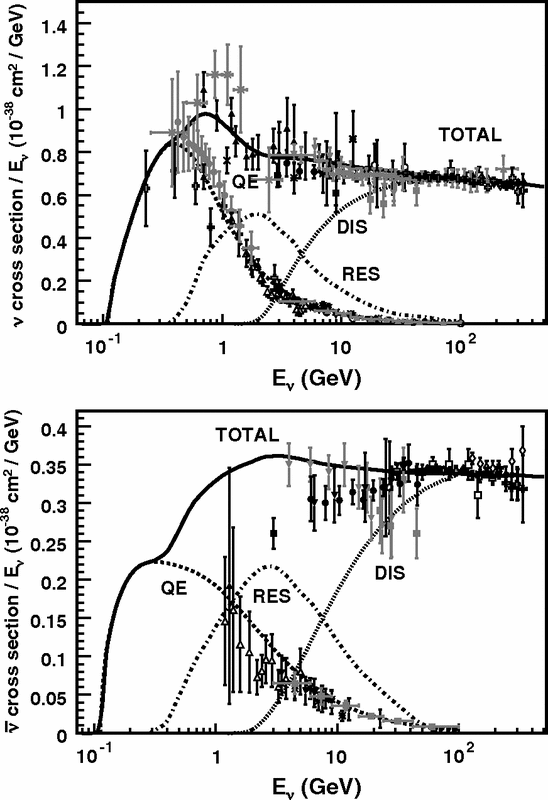
\includegraphics[width=0.48\textwidth,keepaspectratio]{neutrino_nucelon_crosssections.png}
  \end{center}
  \caption{Total inclusive cross-section is plotted above as a function of energy along with individual cross-sections for different interaction channels. Above a few tens of GeV, it's clear that deep inelastic scattering begins to dominate \cite{2012RvMP...84.1307F}.}
  \label{fig:neutrino_scattering}
\end{wrapfigure}

In the elastic (NC) or quasi-elastic (CC) scenario, an incoming neutrino will scatter off of the nucleon as a whole imparting some of its energy to the target. This is usually sufficient to eject the target nucleon and in some cases additional nucleons from the nucleus. The CC scattering is referred to as quasi-elastic due to the fact that it requires the conversion of the target proton(neutron) into a neutron(proton) to ensure charge conservation. This type of scattering does not probe the internal constituents of the nucleus (quarks and gluons collectively referred to as partons). The absolute cross-section, however, will depend heavily on nuclear properties of the target atom. Examination of Figure \ref{fig:neutrino_scattering} shows that even in a DeepCore dominated event sample this process will very rare given the threshold for neutrino detection is approximately 10 GeV.

Above 1 GeV in neutrino energy, resonance production overtakes quasi-elastic scattering in relative contribution to the total interaction cross-section. In this form of inelastic scattering, the momentum transfer provided by the neutrino collision can excite the nucleon target. The decay of this excited state will generally involve the emission of an energetic meson (a particle consisting of a quark-anti-quark pair). At lower energies the emitted meson will usually be a single pion ($\pi^{+},\pi^{-}$), however at higher energies multiple pions can be produced as well as strange mesons such as the kaon. An example muon neutrino resonance interaction takes the following form:

\begin{eqnarray}
\nu_{\mu} + N \rightarrow \mu^{-} + N^{*} \rightarrow \mu^{-} + N + \pi^{+}
\end{eqnarray}
In the scenario described above, the exited nucleon \textit{N} decays and emits a charged pion. Other end states yielding either charged or neutral pions are possible as well for either CC or NC interactions. An additional possibility is coherent scattering with the entirety of the nucleus. The momentum transfer in this case is rather low and results in little nuclear recoil and a heavily forward-scattered pion.

As the momentum transfer in the interaction increases, more exotic resonances can arise which in turn can result in the production of multiple pions or heavier mesons. The large number of possible end states for these interactions makes proper simulation of the process complicated. This can be significant for specialized analyses focusing on the lowest energy events in DeepCore as neutrinos interacting via resonance production actually make a sizable contribution to the event sample. What is ultimately important, however, is that the total light yield from these interactions is estimated correctly by the simulation used for analysis purposes. While elastic scattering and resonance production are significant for the lowest energy analyses or possible future low energy extensions for IceCube, these processes only add a minor contribution to the event sample used in the analysis presented in this thesis.

\subsection{Deep Inelastic Scattering}
The most important neutrino-matter interaction for IceCube is that of deep inelastic scattering. As Figure \ref{fig:neutrino_scattering} shows, it is far and away the dominant mode of interaction for neutrinos above the threshold energy for detection in IceCube ($\sim$100 GeV). At these energies, the wavelength of the incoming neutrino becomes sufficiently small enough to begin probing the internal parton structure of the target proton or neutron. The energy imparted to these internal components will break the nucleon apart. This breakup will result in the formation of a shower of short-lived hadrons (a particle composed of quarks) which will decay into more stable particles. The generation of these hadronic cascades during nucleon breakup is often referred to as hadronization of the nucleon's constituent quarks, and the formation of these particles is necessitated by quark confinement, a property of the strong nuclear interaction. The particles within this shower will suffer energy losses through either collisions or ionization of surrounding material until the energy is fully dissipated. A diagram detailing the deep inelastic scattering process for a muon neutrino is shown in Figure \ref{fig:dis_scattering}.

\begin{figure}[ht]
  \begin{center}
    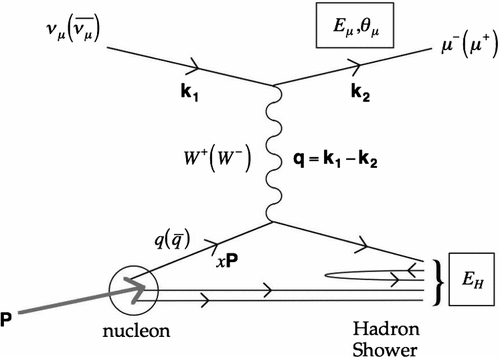
\includegraphics[width=0.7\textwidth,keepaspectratio]{dis.png}
  \end{center}
  \caption{Feynman diagram of a $\nu_{\mu}$ undergoing deep inelastic scattering with a nucleon via charged-current interaction. A large momentum exchange through a charged $W$ boson leads to breakup of the nucleon \cite{2012RvMP...84.1307F}.}
  \label{fig:dis_scattering}
\end{figure}

Like the scattering modes mentioned earlier, deep inelastic scattering can occur through either a CC or NC interaction. The hadronic shower will occur regardless of the interaction mode, while an end-state lepton will only be present in the CC scenario. Neutrino experiments can infer the properties of the interacting neutrino through examination of the end state products. The three possible leptons (e$^-$, $\mu$, $\tau$) produced in CC interactions each exhibit different behavior as they interact in the detection medium allowing for flavor identification of the original neutrino. In the case of NC scattering, however, only the hadronic cascade is observable by the experiment. This not only prevents flavor identification of the neutrino, but it also makes estimation of the neutrino energy very difficult as some fraction of the total energy is carried away by an outgoing neutrino.

\begin{figure}[ht]
\centering
\begin{minipage}[b]{0.45\linewidth}
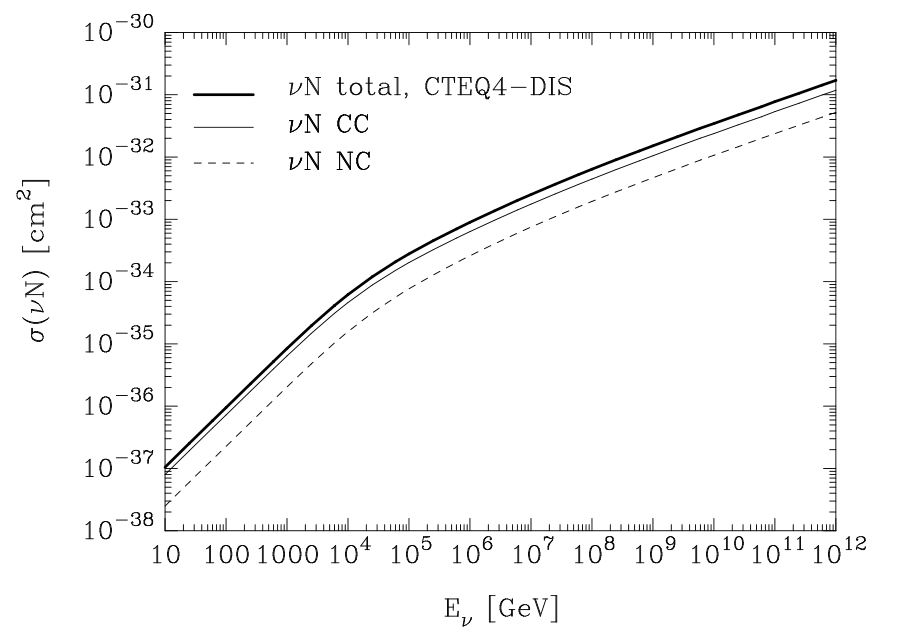
\includegraphics[width=0.95\textwidth]{DIS_CS_Neutrino.png}
\caption{Charged current (thin), neutral current (dashed), and total inclusive (solid) deep inelastic scattering cross-section by energy for neutrinos \cite{Gandhi:1998ri}.}
\label{fig:NeutrinoDIS_CS}
\end{minipage}
\quad
\begin{minipage}[b]{0.45\linewidth}

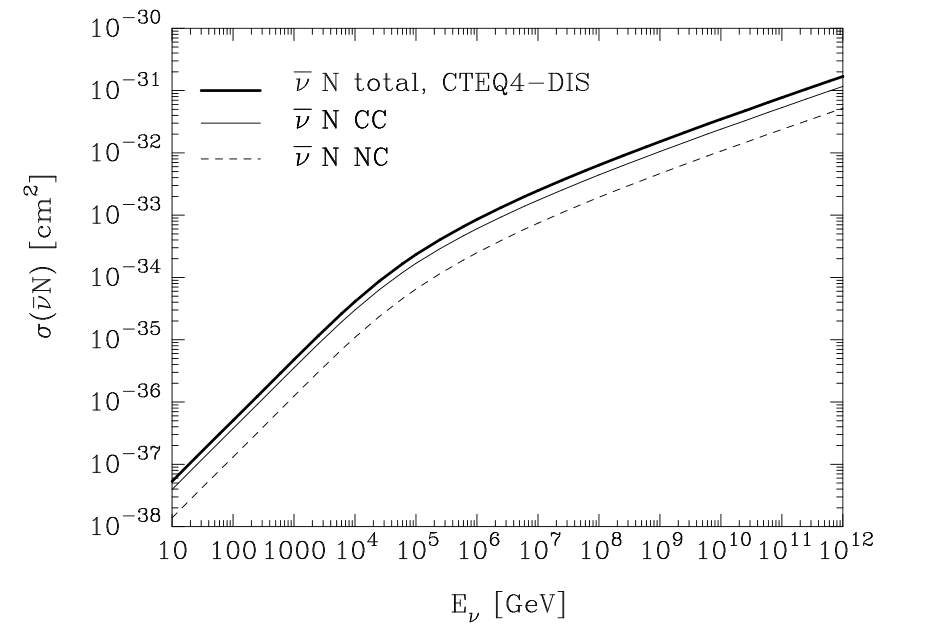
\includegraphics[width=1.0\textwidth]{DIS_CS_AntiNeutrino.png}

\caption{Charged current (thin), neutral current (dashed), and total inclusive (solid) deep inelastic scattering cross-section by energy for anti-neutrinos \cite{Gandhi:1998ri}.}
\label{fig:AntiNeutrinoDIS_CS}
\end{minipage}
\end{figure}

The cross-section for deep inelastic scattering increases with increasing neutrino energy as Figures \ref{fig:NeutrinoDIS_CS} and \ref{fig:AntiNeutrinoDIS_CS} show. While this increasing cross-section is generally favorable for detection purposes due to higher probability to interact in neutrino telescopes, a larger interaction cross-section at higher energies also leads to absorption of neutrinos within the Earth. Absorption is fairly infrequent for neutrinos below 10 TeV, but it becomes increasingly relevant for astrophysical neutrinos at the PeV or EeV scale \cite{2013arXiv1304.4891K}.

\subsection{Propagation of Interaction Products}
The products leftover from high-energy neutrino-nucleon interactions are generally very energetic as well. These particles will subsequently undergo many forms of energy loss and possibly decay as they travel through a detection medium. In a given interaction, the total light yield and its spatial extent are contingent on the products of the interaction. The products themselves are ultimately determined by both the flavor of the primary neutrino and whether the neutrino interaction was of the charged- or neutral-current variety. This section will detail the important energy loss mechanisms for interaction products and how these losses produce an observable signal in the IceCube detector. There are many modes of interaction for charged particles in materials some of which are highly energy dependent and stochastic in nature. Because IceCube was designed specifically to detect and track high energy muons, the description of energy loss mechanisms will primarily focus on how these mechanisms pertain to muons. The same interactions will occur for other charged particles produced in neutrino interactions, however, these particles fail under normal circumstances to produce tracks long enough to be resolved by IceCube.

The primary energy loss mechanisms for charged leptons are ionization, bremsstrahlung, pair-production, and photo-nuclear interactions \cite{2001PhRvD..63i4020I}. These losses are described below:

\begin{adjustwidth}{2.5em}{2.5em}
\setlength{\parindent}{0pt}
\textbf{Ionization} - Ionization energy losses occur as the charged particle transfers energy to the electrons of intervening atoms and molecules. This energy loss is fairly continuous and is the dominant loss mode for sub-TeV muons in the ice \cite{2001ADNDT..78..183G}.

\textbf{Bremsstrahlung} - Energy losses via bremsstrahlung involve the deflection of the particle by another charged particle (typically a positively charged nucleus). This deflection results in the emission of a photon with energy equivalent to the kinetic energy lost in the interaction. These photons can often be energetic enough to produce a electromagnetic shower through electron-positron pair-production.

\textbf{Pair-production} - As the name might suggest, pair-production is the process in which an electron-positron pair is produced in the Coulomb field of an atomic nucleus \cite{2001ADNDT..78..183G}. If the energy imparted to the electron-positron pair is large enough, an electromagnetic shower can be produced.

\textbf{Photo-nuclear} - At high energies, charged leptons can undergo inelastic scattering with nuclei and in the process create hadron showers \cite{2003PhRvD..67c4027B}. The process is similar to the neutrino-nucleon scattering processes described earlier but with photon-exchange taking place rather than $W$ or $Z$ boson exchange.
\end{adjustwidth}
\setlength{\parindent}{17.5pt}
The relative contribution to total energy loss these interactions provide will vary with particle energy. In practice, this is commonly parameterized so the average range of the particle in a given medium can be more easily computed \cite{2001ADNDT..78..183G}:
\begin{equation}\label{eq:stopping_power}
-\frac{dE}{dX} = a(E) + b(E) E
\end{equation}
Here $a(E)$ represents the more or less continuous energy losses from ionization (electron stopping power) while the $b(E)$ term includes the contributions from the various radiative energy loss processes (bremsstrahlung, pair-production, and photo-nuclear). The relative strength of these processes with respect to stopping power can be seen in Figure \ref{fig:MuonStoppingPower}. By integrating the stopping power from Eq. \ref{eq:stopping_power}, we arrive at the following expression for particle range
\begin{equation}\label{eq:range}
R(E) = \int_{E_0}^{E}[a(E') + b(E')E']dE'
\end{equation}
with $E_0$ being the final energy of the particle \cite{2001ADNDT..78..183G}.
With a few approximations Eq. \ref{eq:range} can be simplified into a simple expression yielding particle range from just the initial energy. Such assumptions must neglect the stochastic nature of many of these energy losses and therefore any range derived this way is more representative of an average range. The most important thing to note is that these losses determine both the brightness and length of muon tracks within the IceCube detector and ultimately how well their direction can be resolved.

\begin{figure}[ht]
  \begin{center}
    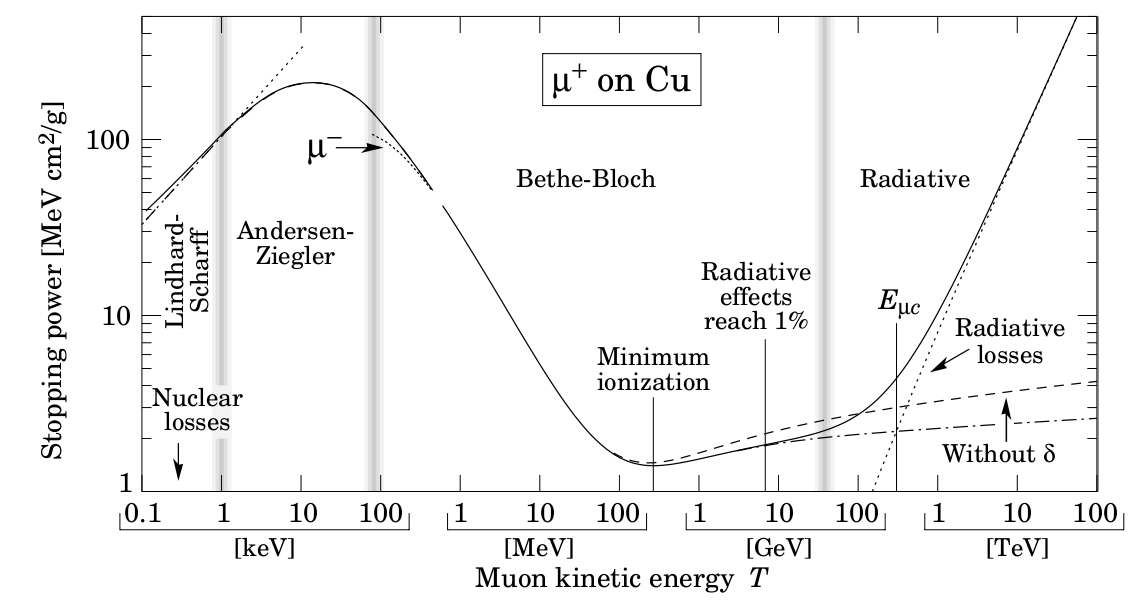
\includegraphics[width=0.9\textwidth,keepaspectratio]{MuonStoppingPower.png}
  \end{center}
  \caption{Total stopping power (solid line) of muons in copper as a function of kinetic energy. Contributions from individual processes are shown as well as the energy ranges in which these processes are most dominant. \cite{2001ADNDT..78..183G}.}
  \label{fig:MuonStoppingPower}
\end{figure}

While the previously described processes are most relevant for particle energy loss, the most import energy loss mechanism for particle detection in IceCube is the production of Cherenkov light. Cherenkov emission only makes a small contribution to total energy loss by charged particles in materials. It does however produce light in the visible spectrum yielding an easily detectable signal. This emission occurs when a charged particle travels through a dielectric medium at a greater speed than the phase velocity of light in that medium. The particle will polarize the surrounding material as it travels, however the particle will have moved on before enough time has elapsed for the material to relax resulting in a build up of wave fronts. A shock front is produced that takes the shape of a cone about the particle track. This light cone has an opening angle given by
\begin{equation}
\cos{\theta}=\frac{1}{n\beta}
\end{equation}
where $n$ is the index of refraction for the material and $\beta$ is the ratio of the particle velocity and the speed of light $c$. If one takes a typical value for the refractive index in ice ($n=1.31$), an angle of roughly $40^{\circ}$ is obtained. Resolution of the Cherenkov cone of a single particle is a powerful identification technique for many particle detectors. However, the Cherenkov light fronts of only the most energetic and long-lived particle tracks are able to be resolved in IceCube due to the large separation distances between individual light sensors.

%% Diagram of Cherenkov Cone?

For most neutrino events in IceCube, deep inelastic scattering with nucleons in the ice via either neutral or charged boson exchange deposits enough energy to cause the breakup of the nucleon target. This breakup will result in the formation of a shower of short-lived hadrons (a particle composed of quarks) which will suffer energy losses and decay into more stable particles. These longer lived particles will dissipate the remaining energy through ionization, bremsstrahlung, pair production, or nuclear interactions until the energy imparted by the neutrino is dissipated. The physical extent of these showers is typically on the order of a few meters, much smaller than the spacing between light sensors in IceCube. All of the energetic particles composing the shower will emit Cherenkov radiation as they propagate in the ice giving a pool of light centered at the interaction vertex whose photon count is proportional to the energy of the interaction.


\section{Flavor Oscillations}
The process in which the lepton flavor of a given neutrino can change during its propagation is one of the particle's more intriguing properties. The unexpected observation of neutrino oscillations indicated that the neutrino, which was initially thought to be massless under the Standard Model, must actually have some non-zero mass after all. Recently, many experiments have studied this phenomenon with high precision in hopes of accurately determining the mass-splitting of the neutrino eigenstates as well as if neutrinos undergo CP violation. While the analysis being presented is in no way suited to studying the oscillation phenomenon, how the results are interpreted is very much dependent on how the modeled neutrino flavor ratio for a source evolves from its origin to its arrival at Earth. Thus, this section will describe in short detail the oscillation process over astronomical baselines and through the Earth, the scenarios most applicable to IceCube.

The mixing of neutrino states arises due to the fact that the neutrino mass eigenstates do not directly correspond to the neutrino flavor eigenstates \cite{1978PhRvD..17.2369W}. While neutrinos are produced through weak interactions giving them a definite lepton flavor state, the mass of that neutrino is actually a superposition of three separate mass states. Likewise, the mass state of the neutrino is given by a superposition of the three lepton states. The phase of the mass states will evolve differently during propagation according to the mass differences between the mass eigenstates. Thus, when the neutrino interacts with matter again via the weak force it may be observed in a flavor state other than the its state during production. This mixing possibility can be described by a mixing matrix $U$:
\begin{equation}
\nu_{\alpha} = \sum_{i=1}^{3} U_{\alpha i} \nu_{i}
\end{equation}
where $\nu_{\alpha}$ are the lepton states ($e^-,\mu,\tau$) and $\nu_i$ are the mass states (1,2,3). Using the notation of Nunokawa et. al \cite{2008PrPNP..60..338N}, the matrix $U$ has the form
\begin{equation}
U = \left(\begin{array}{ccc}
1 & 0 & 0 \\
0 & c_{23} & s_{23} \\
0 & -s_{23} & c_{23}
\end{array}\right)
\left(\begin{array}{ccc}
c_{13} & 0 & s_{13}e^{i\delta} \\
0 & 1 & 0 \\
-s_{13}e^{i\delta} & 0 & c_{13}
\end{array}\right)
\left(\begin{array}{ccc}
c_{12} & s_{12} & 0 \\
-s_{12} & c_{12} & 0 \\
0 & 0 & 1
\end{array}\right)
\end{equation}
\begin{equation}
=
\left(\begin{array}{ccc}
c_{12}c_{13} & s_{12}c_{13} & s_{13}e^{i\delta} \\
-s_{12}c_{23}-c_{12}s_{23}s_{13}e^{i\delta} & c_{12}c_{23}-s_{12}s_{23}s_{13}e^{i\delta} & s_{23}c_{13}\\
s_{12}s_{23}-c_{12}c_{23}s_{13}e^{i\delta} & -c_{12}s_{23}-s_{12}c_{23}s_{13}e^{i\delta} & c_{23}c_{13} \\
\end{array}\right)
\end{equation}
In the above, $c_{ij}$ and $s_{ij}$ are shorthand notation for cos $ \theta_{ij}$ and sin $\theta_{ij}$ respectively while the $\delta$ term is related to charge-parity (CP) violation. By taking the inner product of the two states after application of the mixing matrix one arrives at Eq. \ref{eq:oscprob} which gives the probability of transition of a neutrino of flavor $\alpha$ to one of flavor $\beta$ during propagation \cite{2008PrPNP..60..338N}.
\begin{equation}\label{eq:oscprob}
P(\nu_{\alpha}\rightarrow \nu_{\beta}) = \left| \sum_{i} U_{\alpha i}^* U_{\beta i} e^{-i\frac{m_{i}^2}{2E}L}\right| ^2
\end{equation}

The full-fledged oscillation probability is complicated, but the most important thing to takeaway from the expression given by Eq. \ref{eq:oscprob} is that the probability of observing the neutrino in a different state depends on the propagation length $L$ and the energy of the particle $E$. In many cases it is possible to only consider a two-flavor oscillation scenario as the third flavor may not participate strongly in the energies and distances being considered. This allows us to reduce the mixing matrix to a two dimensional form making the expression for oscillation probability much simpler \cite{1998PhRvL..81.1562F}:
\begin{equation}\label{eq:2doscprob}
P(\nu_{\alpha}\rightarrow \nu_{\beta}) = sin^22\theta sin^2\left(\frac{1.27\Delta m^2 (eV^2) L (km)}{E_\nu (GeV)}\right)
\end{equation}
This formulation will yield the probability of oscillation provided you know the mixing angle $\theta$ between $\alpha$ and $\beta$ and the mass-squared difference $\Delta m^2$ for the neutrino mass eigenstates. This approximation is commonly used by several experiments (e.g. IceCube \cite{2013PhRvL.111h1801A}) to make measurements on specific mixing angles. The current best-fit values for neutrino oscillation parameters are given in Table \ref{tab:osc_param}.




\begin{figure}[ht]
  \begin{center}
    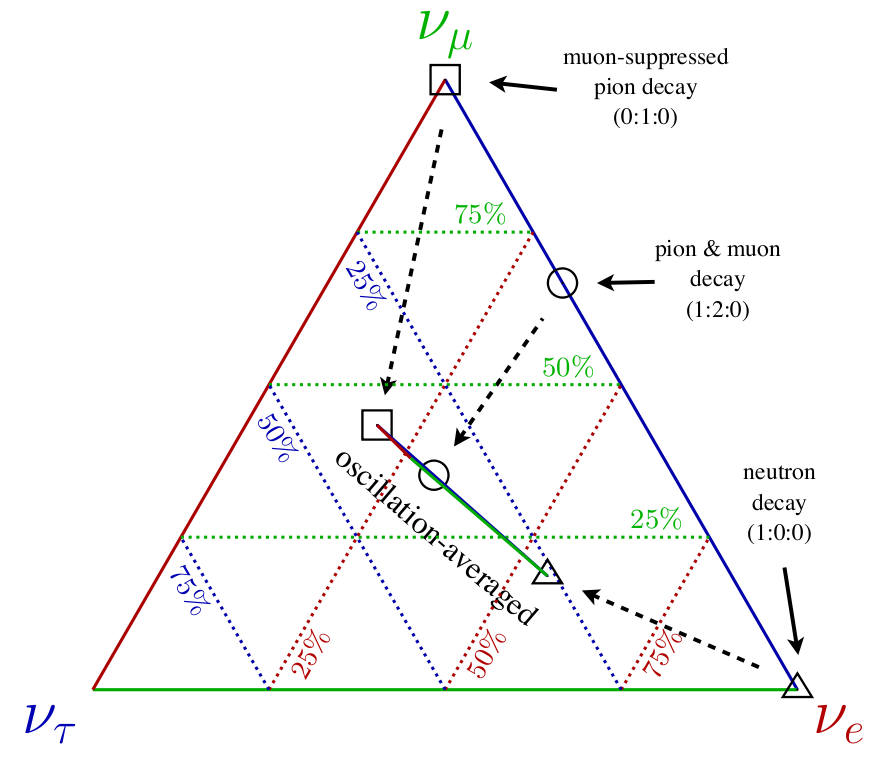
\includegraphics[width=0.75\textwidth,keepaspectratio]{AstroBaselineOsc.png}
  \end{center}
  \caption{Neutrino flavor ratio space. Oscillation over astronomical baselines will result in a flavor ratio at Earth different than at source. If the flavor ratio for a given source can be measured it can help identify the process through which that source's neutrinos were produced \cite{2014arXiv1412.5106I}.}
  \label{fig:baseline_osc}
\end{figure}

[MSW]

\chapter{Neutrino Astronomy}
As the name suggests, the field of neutrino astronomy is concerned with the detection of neutrinos of extraterrestrial origin for the use of identifying and classifying astrophysical sources. In a similar fashion to the advances made through expansion of traditional optical astronomy to the high-energy regime of x-rays and gamma-rays, it is thought that the unique window provided by neutrino astronomy can facilitate tremendous increases in our understanding of the universe. However, the detection of astrophysical neutrino events presents a exceedingly difficult challenge with detection of an appreciable number of neutrinos from a single source requiring enormous instrumented volumes. Therefore, it is relevant to discuss the potential scientific rewards neutrino astronomy can provide.

\section{Motivation}
Neutrinos provide a novel and unperturbed view into furthest reaches of the universe. 
The detection of a neutrino flux from a source and measurement of its spectrum would provide critical insight into the processes governing the densest and most energetic regions of that object.

[Illustration of different messengers]
[ Cosmic ray -- Neutrino Connection]
\begin{figure}[ht]
  \begin{center}
    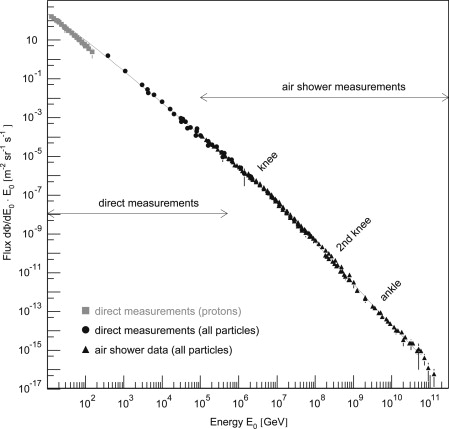
\includegraphics[width=0.85\textwidth,keepaspectratio]{CosmicRaySpectrum.jpg}
  \end{center}
  \caption{Cosmic ray energy spectrum at Earth as measured by several experiments \cite{2009PrPNP..63..293B}.}
  \label{fig:cosmicray_spec}
\end{figure}

[What can neutrino astronomy reveal?]

\section{Detection Methods}

The primary method for the detection of high-energy neutrinos is through observation of Cherenkov light produced by interaction secondaries in a transparent medium (typically water or ice). Events can be detected either by surrounding a detection volume with light detectors (as is the case for Super-Kamiokande \cite{?}) or by placing the detectors within the detection medium itself (e.g. IceCube, ANTARES).

[Not a lot to this section...]
\chapter{Neutrino Sources}
While no individual extra-solar high-energy neutrino sources have yet to be discovered (with the exception of SN 1987A), there is strong theoretical support  and indirect observational evidence for their existence. The measurement of extremely high-energy cosmic rays implies that a flux of energetic neutrinos must also be present due to the intimate link between hadronic acceleration and neutrino production in high-energy astrophysical environments. Most importantly, the recent discovery of a flux of high-energy neutrinos of astrophysical origin by IceCube \cite{2013Sci...342E...1I} provides confirmation that there must be some sources of high-energy neutrinos though they may be very diffuse.


[Finish section intro]

\section{Active Galactic Nuclei}
[Talk about neutrinos from AGN flares? Probably don't need much on this.]

\section{Core-Collapse Supernovae}
The detection of several neutrino events in temporal coincidence with supernova 1987A marked the first detection of an extra-solar neutrino source. Neutrino events were observed in three separate detectors a few hours prior to the optical observation. Such an observation was possible due to the close proximity of the progenitor which was located within the Large Magellanic Cloud ($\sim$50 kpc from Earth). Detection of these events confirmed the theoretical prediction of an enormous liberation of energy in the form of neutrinos during the collapse of the core of a massive star.


%% neutrino production from neutron conversion, SN1987A
%% Too low energy in IceCube, but SNDAQ
\begin{wrapfigure}{r}{0.5\textwidth}
  \begin{center}
    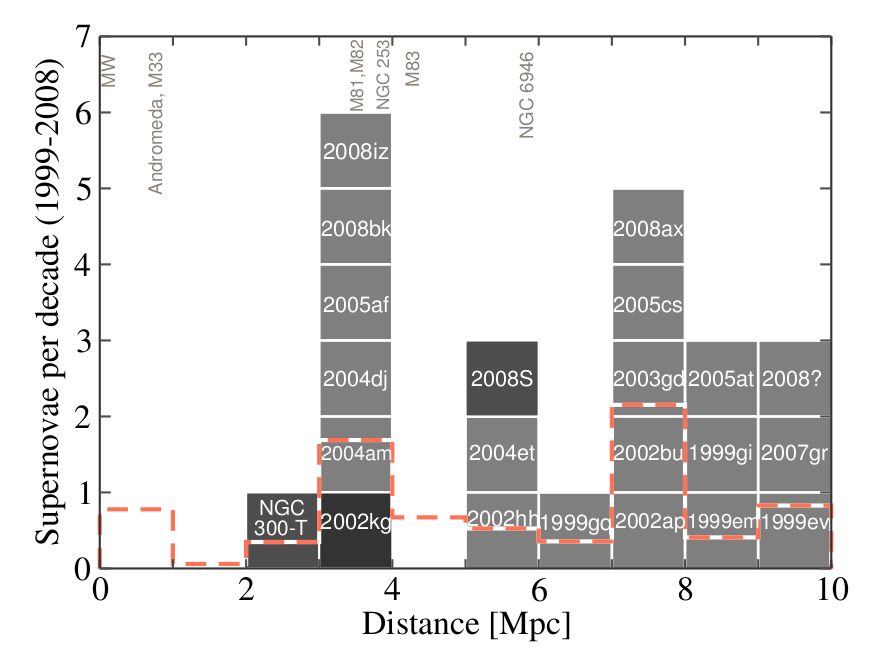
\includegraphics[width=0.48\textwidth,keepaspectratio]{NearbySNCatalogue.png}
  \end{center}
  \caption{Observed SNe within 10 Mpc in the years 1999-2008 \cite{2011PhRvD..83l3008K}}
  \label{fig:local_ccsne}
\end{wrapfigure}


\section{Gamma-ray Bursts}
Gamma-ray Bursts (GRBs) have been considered as a possible source for the most energetic of cosmic rays. Certain cosmic ray acceleration models also suggest that GRBs are prominent neutrino sources as well.
\subsection{Fireball Model}
%% Fireball model, neutrino production in jets


\subsection{Subphotospheric Model}
%% subphotospheric model

\begin{figure}[ht]
  \begin{center}
    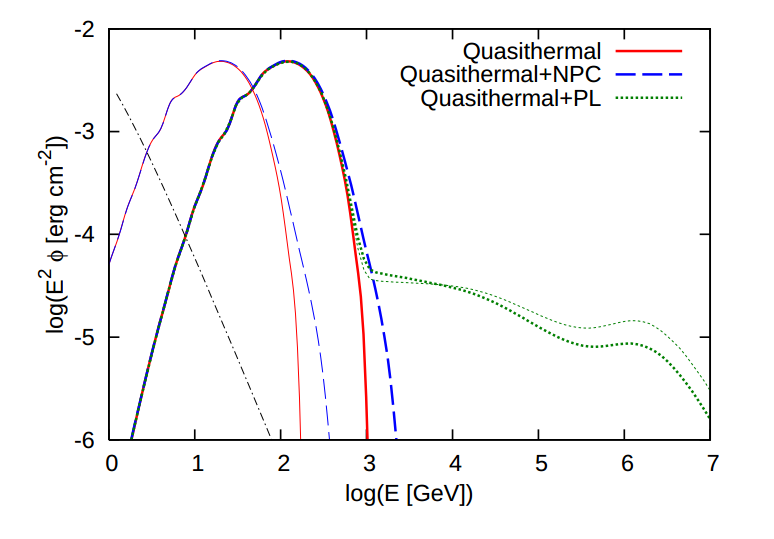
\includegraphics[width=0.85\textwidth,keepaspectratio]{SubPhotoFluence.png}
  \end{center}
  \caption{Energy fluence of $\nu_{\mu}$ and $\bar{\nu}_{\nu}$ from high-luminosity GRB at a redshift of z=0.1 in the sub-photospheric emission model \cite{2013PhRvL.111m1102M}.}
  \label{fig:subphotospheric_nus}
\end{figure}


\section{Choked Gamma-ray Bursts}
The core-collapse of a massive star is thought to be the mostly likely engine for powering the jets responsible for gamma-ray emission from long duration GRBs \cite{2004RvMP...76.1143P}. This suggests that a correlation between long duration GRBs and supernovae should exist. In fact, some instances of GRB association with SNe have been observed \cite{2006ARA&A..44..507W}, \cite{2011AN....332..434M}. This has led some to speculate that jet production during core-collapse might occur in a higher fraction of SNe than the observed GRB-SNe fraction would indicate. Gamma rays from these jets may be hidden from direct observation because they are insufficiently energetic to breakout from the surrounding stellar envelope of the progenitor and are effectively 'choked' off. However, if these jets produce neutrinos in the same manner as the jets in GRBs, it may be possible to observe such a source through its neutrino emission despite the fact that the optical signature remains hidden. In this scenario, a continuum class of objects would exist in which GRBs represent CC-SNe harboring the most energetic of jets.

The observed frequency of CC-SNe in the universe is much higher than that of GRBs \cite{0004-637X-738-2-154}, \cite{2004RvMP...76.1143P}. Because choked GRBs may occur at a much higher rate in the nearby universe, they are a prime target for time-dependent neutrino analyses. 

\subsection{Neutrino Emission Model}
[Primary source of interest. Should be most detailed neutrino source section]
\subsection{Model Limits on SN2008D}
The X-ray telescope of the \textit{SWIFT} satellite detected a bright flash indicating a transient event during observation of NGC 2770 on January, 9, 2008. Followup observations showed that the \textit{SWIFT} source was a core-collapse supernova of type Ib \cite{2008Natur.453..469S}. At a distance of only 27 Mpc, this supernova provided an opportunity for the IceCube detector to search for any corresponding high-energy neutrino emission. There is no clear evidence, however, that SN2008D had an aspherical explosion suggesting the production of jets similar to those described by the RMW/AB model \cite{2008Natur.453..469S}. Nonetheless, a search for emission was carried out using the 22-string partial configuration of IceCube \cite{2011A&A...527A..28I}.

\chapter{Detector}
\section{IceCube and IceTop}
The IceCube Neutrino Observatory is a km$^{3}$-scale neutrino detector located deep within the glacial ice of the Antarctic ice sheet at the geographical South Pole. This location provides IceCube with a pristine detection medium in addition to mechanical support for the entirety of the array. The detector consists of 5,160 light sensors known as digital optical modules (DOMs) which are distributed along 86 cables (referred to as strings) that supply power and provide communication to the surface. Each cable is instrumented with 60 DOMs spaced 17 meters apart starting at 1450 meters below the surface and terminating at 2450 meters below. An inter-string spacing of 125 meters on average results in a total instrumented volume of approximately 1 km$^{3}$. Figure \ref{fig:icecube} provides a schematic illustrating the detector geometry.

\begin{figure}[ht]
  \begin{center}
    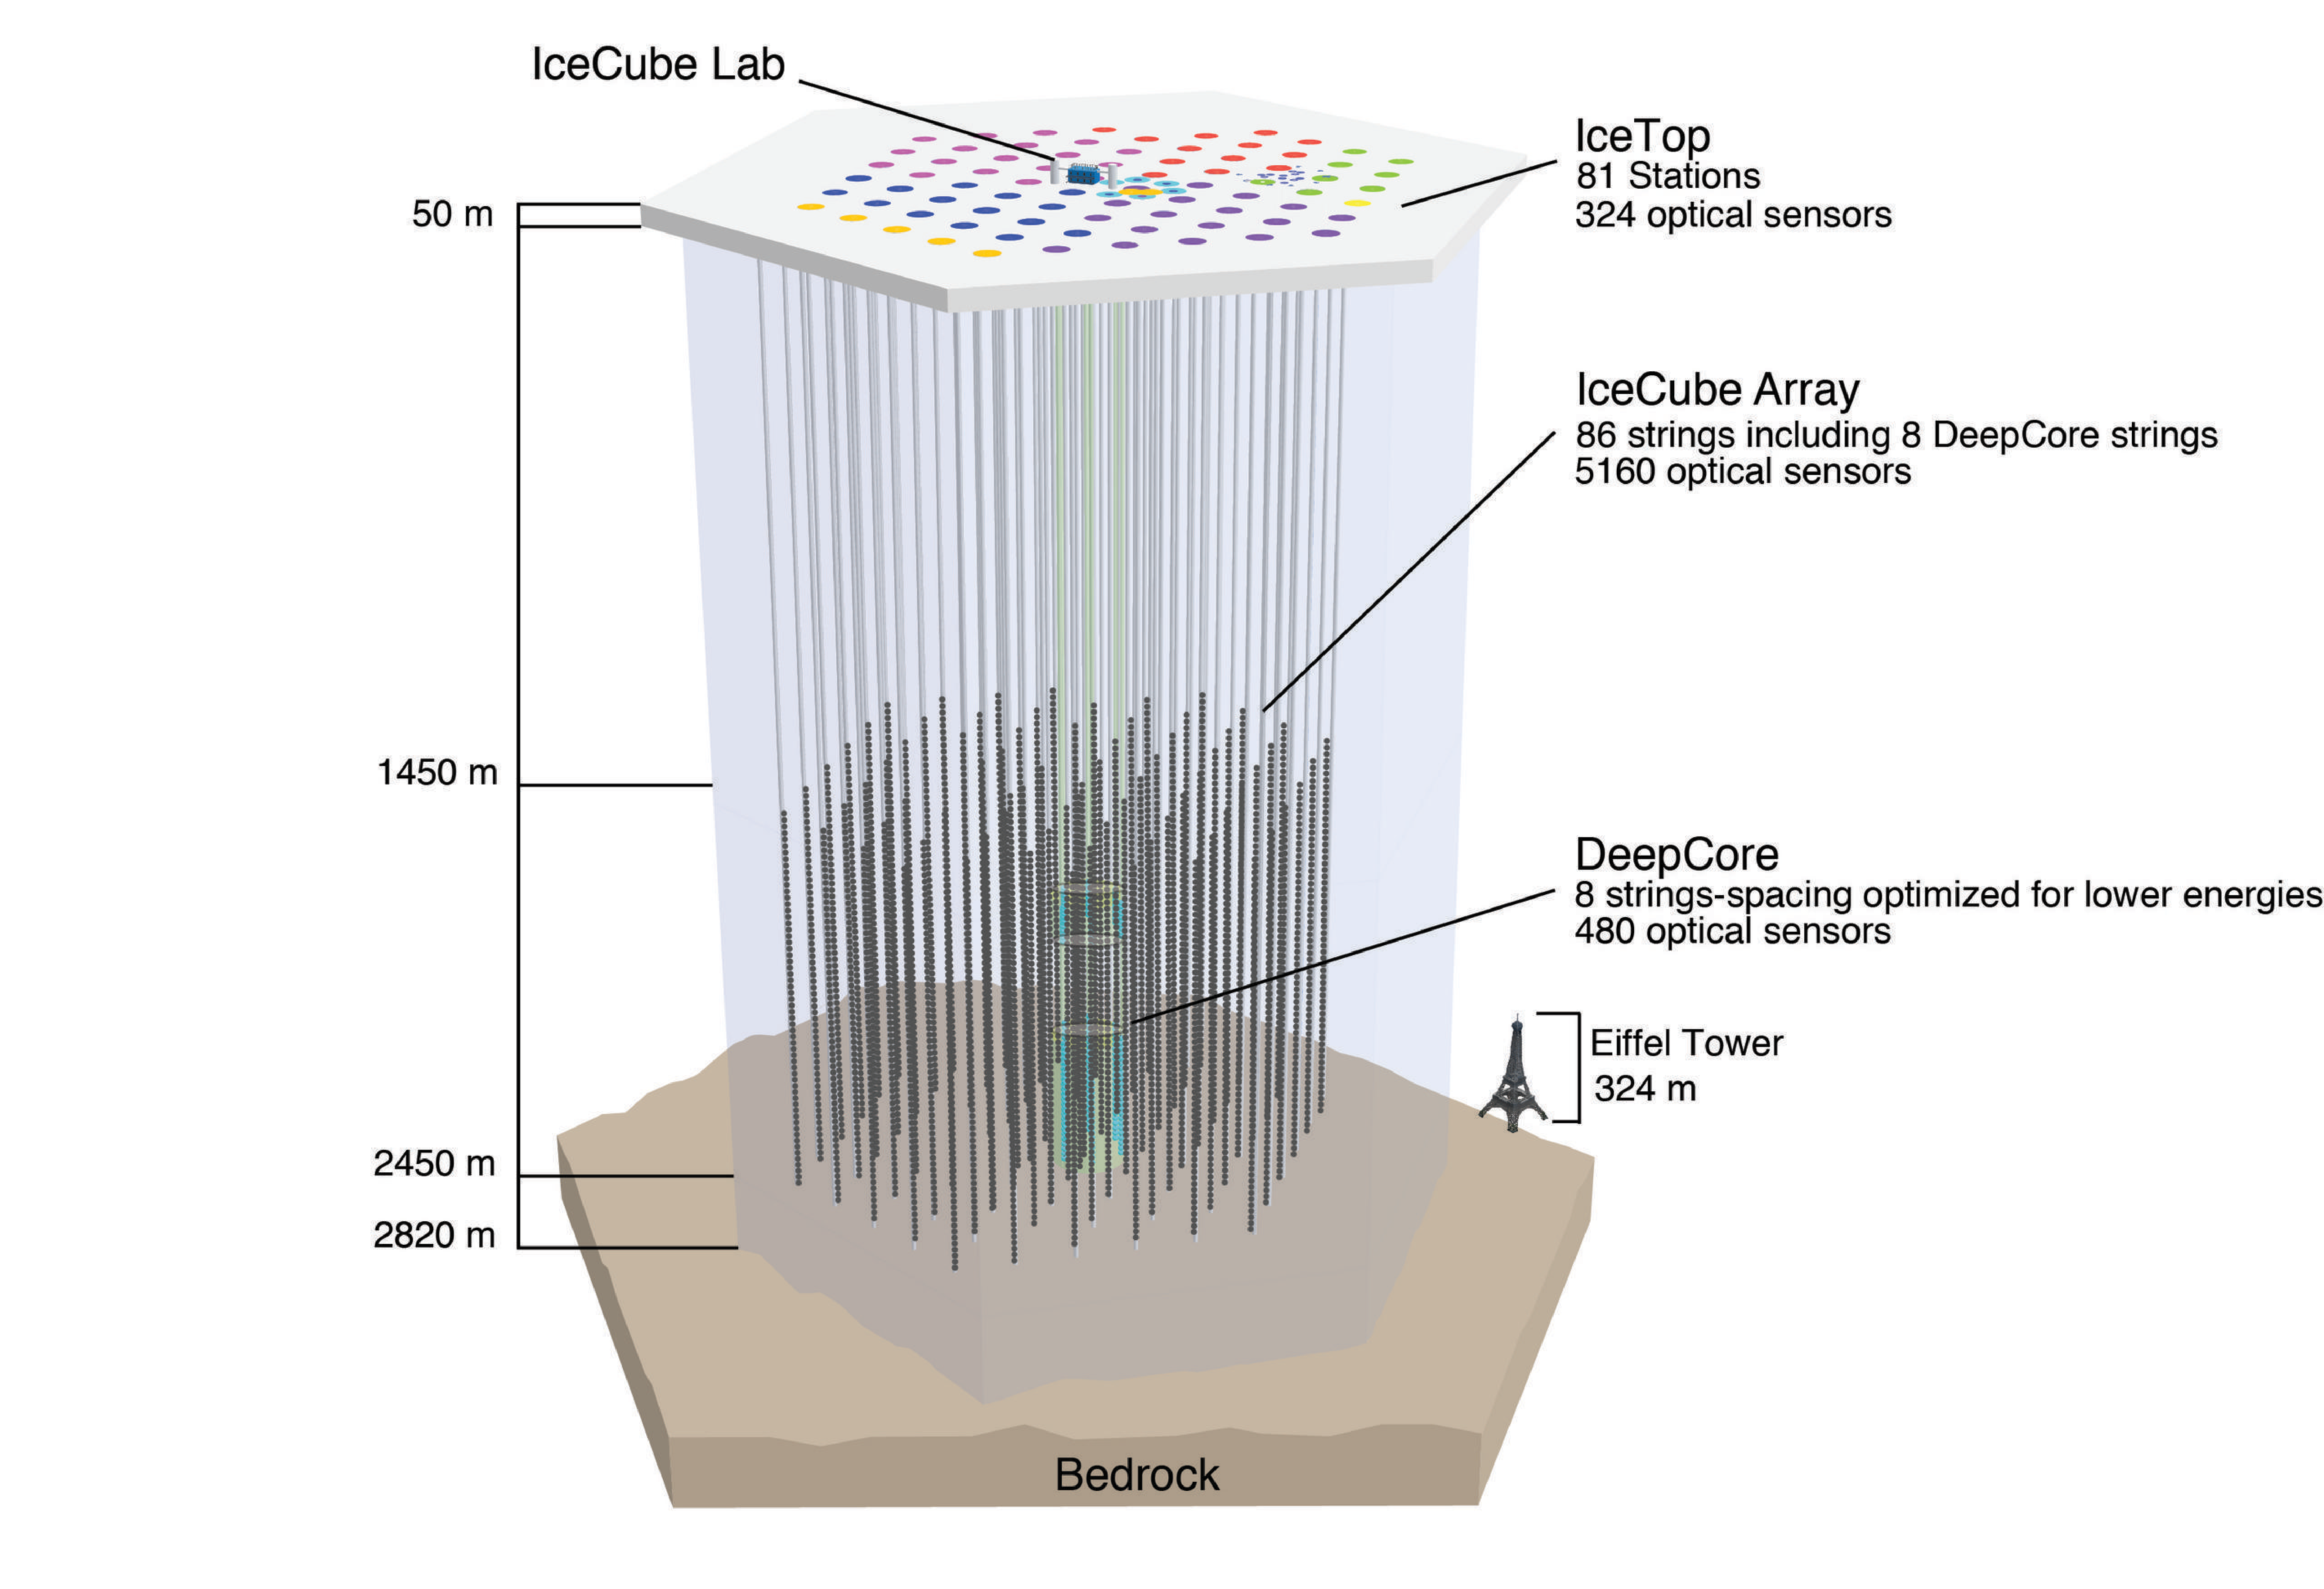
\includegraphics[width=1.0\textwidth,keepaspectratio]{ArrayWSeasonsLabels.pdf}
  \end{center}
  \caption{Diagram of the IceCube Neutrino Observatory (Courtesy of the IceCube Collaboration).}
  \label{fig:icecube}
\end{figure}

Installation of the IceCube strings took place over several years and required the use of a specialized hot-water drill. In the deployment process, the hot-water drill is used to bore through the ice leaving a water-filled column in which the string and its attached DOMs are lowered. The water column subsequently freezes the cable and all DOMs in place rendering them completely inaccessible from the surface. The deployment of the first IceCube string occurred on January 29th, 2005. The remaining strings were deployed over the next five summer seasons resulting in data seasons of different detector shapes and size. The final string was deployed on December 18, 2010 giving IceCube its ultimate 86-string configuration.

%%% IceTop

In addition to the detectors installed deep in the ice, there are also 81 surface detector stations (each station consisting of two tanks) at the surface. These tanks, which utilize two of the same light-sensing DOMs as IceCube, comprise the IceTop surface array. The DOMs in these tanks, which are also frozen in place, look for Cherenkov radiation produced by cosmic ray air shower secondaries in the tank ice. By examining the arrival time of charged particles from the shower front, the direction of cosmic rays incident at Earth can be determined. The spatial extent of the shower as well as the total charge deposition in tank PMTs allows for accurate estimation of the energy of the primary cosmic ray. Data produced from IceTop is used to study cosmic ray composition, spectra, and anisotropy.

Due to the spatial relation of both IceTop and IceCube, they are able to complement the capabilities of each other quite nicely. IceTop's primary purpose is to study air shower physics, but it also serves as a veto for downgoing atmospheric muons and neutrinos in IceCube. This is particularly useful in the search for highly energetic neutrinos of astrophysical origin such as the events reported in \cite{2013Sci...342E...1I} and \cite{2014PhRvL.113j1101A}. Any downgoing events found by these searches that is accompanied by a causually connected air shower signal in IceTop is immediately identified as atmospheric in origin. Alternatively, the background muons detected in IceCube can be used for more detailed study of air shower composition and energy in IceTop analyses. For more detailed information on the physics goals and detection capabilities of IceTop, see \cite{2013NIMPA.700..188A}.


\section{DeepCore}

DeepCore \cite{2012APh....35..615A} is a sub-detector deployed in tandem with IceCube between 2009 and 2010 primarily designed to lower the energy threshold of IceCube. The array consists of eight infill strings located in the center of the IceCube detector in addition to the first layer of surrounding standard IceCube strings. This configuration gives DeepCore three layers of IceCube strings to use as an active veto for the primary background of atmospheric muons. In order to improve detector response to lower energy neutrinos, $\mathcal{O}$(10-100 GeV), the infill strings of DeepCore have a much closer inter-string separation (~42 m) and have 50 DOMs spaced 7 m apart deployed deep in the ice between 2100 m and 2450 m. This denser instrumentation allows for better timing and spatial resolution of charged secondaries produced in neutrino interactions. Additional sensitivity to lower energies is gained throug the use of the newer Hamamatsu R7081MOD model PMT in the infill string DOMs as opposed to the standard Hamamatsu R7081-02 used in IceCube. This model boasts higher quantum-efficiency in the photocathode for photons at typical Cernkov wavelengths ($\lambda \sim 400$ nm). In-ice measurements of the high quantum efficiency (HQE) DOMs showed a 35$\%$ increase in sensitivity to Cherenkov light with respect to the standard IceCube DOMs \cite{2012APh....35..615A}.

\begin{figure}[ht]
  \begin{center}
    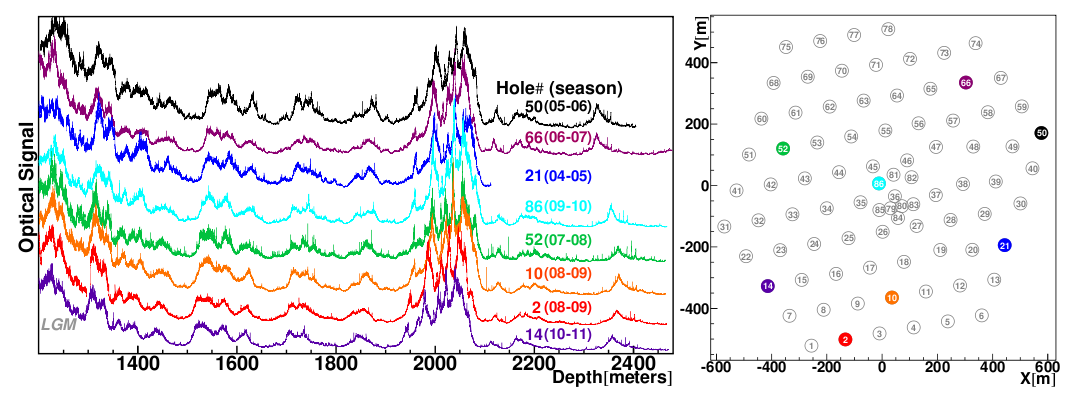
\includegraphics[width=0.98\textwidth,keepaspectratio]{BoreholeLaserDustLogging.png}
  \end{center}
  \caption{Borehole laser measurements of dust concentrations in the ice as a function of depth. Measurements for several IceCube strings are displayed. Higher values on the y-axis denote higher dust concentrations. The "dust layer" features quite prominently at a depth of 2100m \cite{2013JGlac..59.1117.}.}
  \label{fig:DustLogger}
\end{figure}

The depth selected for deployment of the DeepCore DOMs was determined via examination of the ice properties previously mapped by both the Anatarctic Muon and Neutrino Detector Array (AMANDA) \cite{2006JGRD..11113203A} and pre-existing IceCube configurations \cite{2013JGlac..59.1117.}. These investigations into the optical properties of the ice revealed that the deepest ice ($\leq$ 2100 m) had superior optical qualities with respect to the ice closer to the surface. Additionally, it was determined that a layer of high dust concentration in which light is scattered and absorbed to a much higher degree exists at a depth of 2000-2100 m (see Figure \ref{fig:DustLogger}). The eight infill strings also have a section of 10 DOMs with 10 m spacing located just above the dust layer. These DOMs form a veto cap to further increase the detection probability and rejection of directly down-going muons. Figure \ref{fig:DeepCoreSchematic} shows the distribution of DeepCore DOMs and the spacing and orientation of the DeepCore strings with respect to IceCube as a whole.

\begin{figure}[ht]
  \begin{center}
    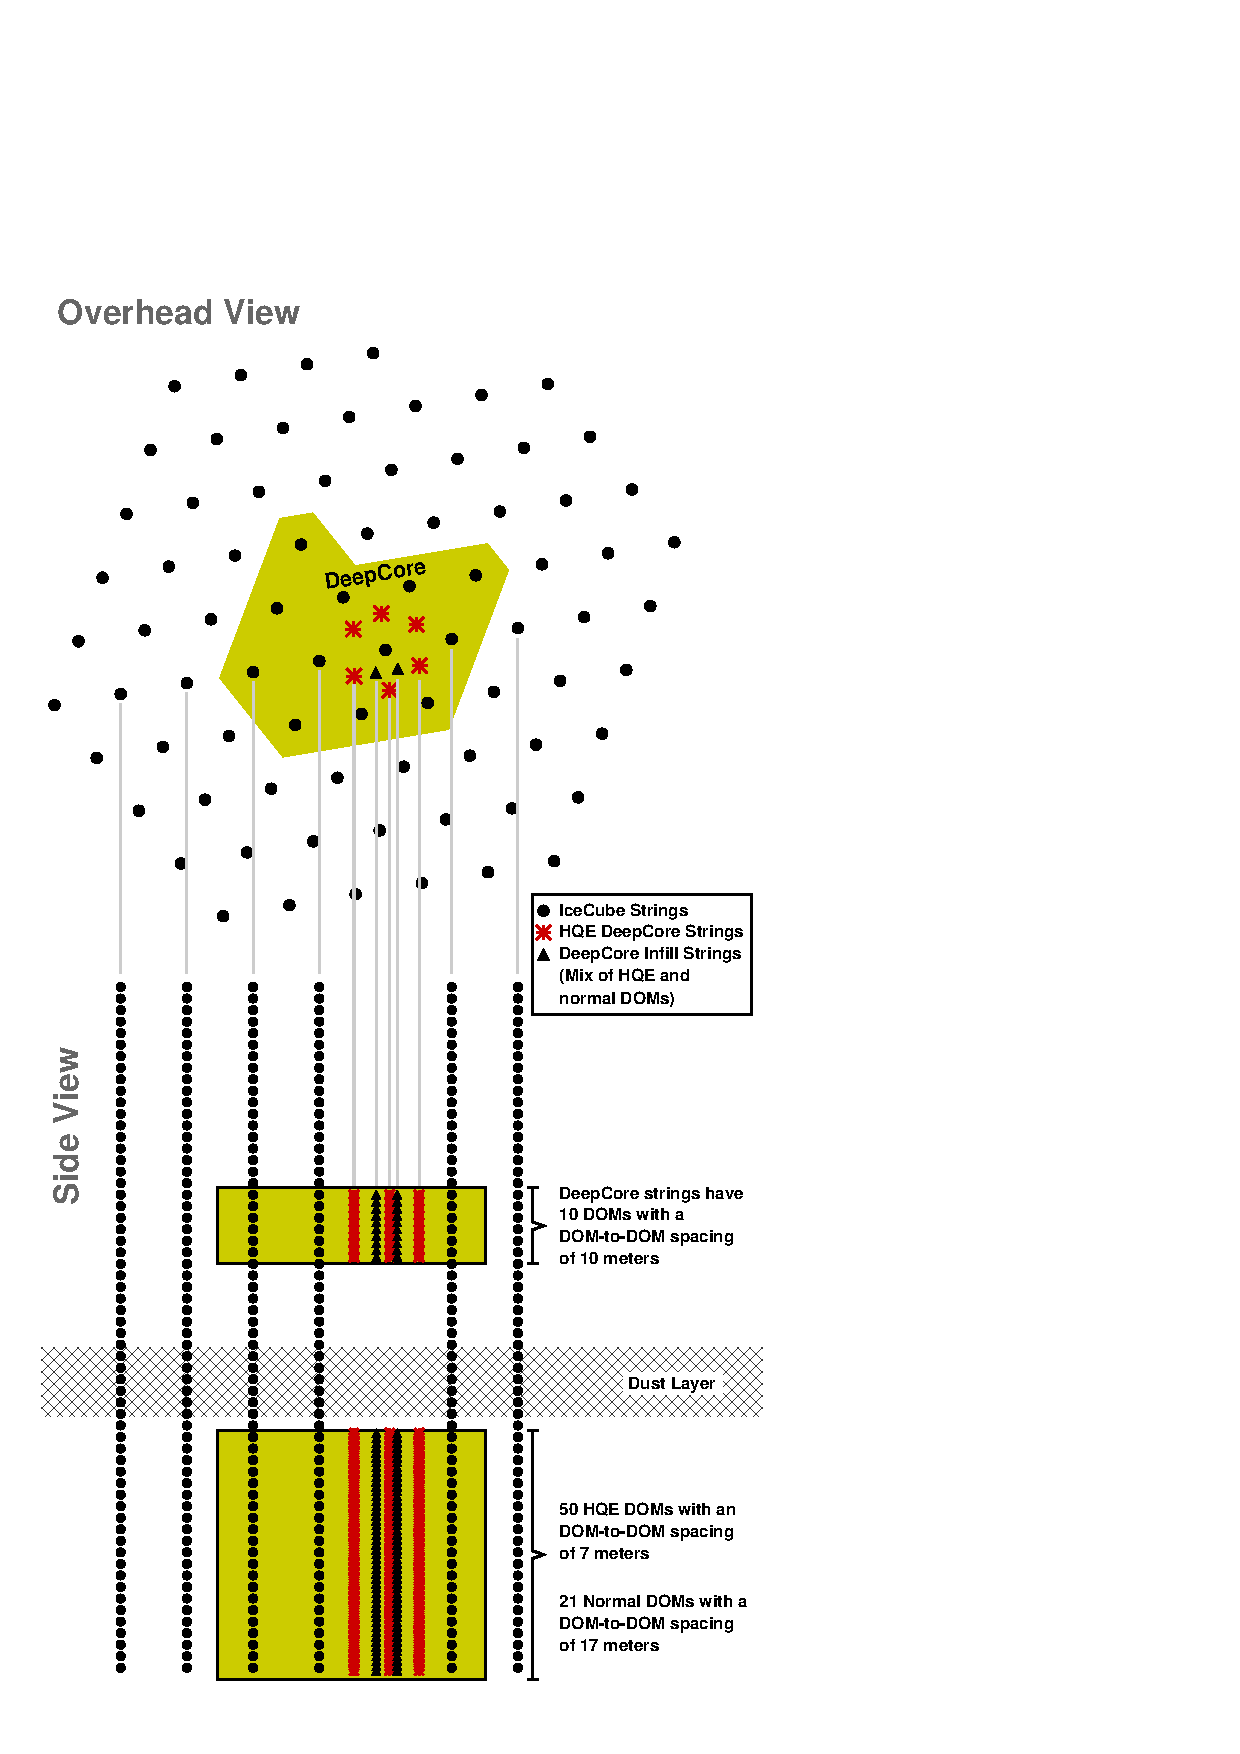
\includegraphics[width=0.7\textwidth,keepaspectratio]{IC86EDC_DeepCoreDiagram.pdf}
  \end{center}
  \caption{Top down and side-view diagram of DeepCore. The side-view shows the difference in DOM distribution for the infill strings and their relation to the dust layer \cite{2012APh....35..615A}.}
  \label{fig:DeepCoreSchematic}
\end{figure}

%%% Physics in DeepCore
The primary physics goal of the DeepCore installation is to provide increased sensitivity for indirect dark matter searches by improving the IceCube detectors ability to resolve sub-100 GeV neutrino events. In this regard, it has been quite successful in establishing limits on the cross-sections of many WIMP (Weakly Interacting Massive Particle) dark matter models with the Sun \cite{2013PhRvL.110m1302A} and Milky Way \cite{2011PhRvD..84b2004A} as possible sources. The lowering of the detector's energy threshold has also made neutrino oscillation parameter measurements possible due to the high statistics provided by atmospheric neutrino events \cite{2013PhRvL.111h1801A}. Most importantly for the analysis presented in this thesis, however, is the improvement in effective area and resolution DeepCore provides for 30-150 GeV muon neutrinos. As this thesis will demonstrate, including these neutrino events into previously established IceCube point source analysis methods greatly improves IceCube's capability to discover transient events with soft spectra.
\section{Neutrino Events in IceCube}

In order to isolate the sparse neutrino events from the abundance of background cosmic ray muons, it is necessary to fully understand the nature of the detector response to neutrinos and neutrino secondaries interacting within the detector. Neutrinos that are sufficiently energetic to be detected by IceCube will undergo deep inelastic scattering with a nucleon target (see for more information on this process see section \textbf{2.1.1}). This process will either be charged-current (CC) or neutral-current (NC) depending on the nature of the boson exchange and the final lepton state. The hit topology of a given neutrino event in IceCube will depend upon the flavor of the neutrino ($\nu_{e}$, $\nu_{\mu}$, $\nu_{\tau}$) as well as the channel through which it interacts with a target nucleon in the ice.

In NC interactions of all flavors, a hadronic cascade is produced which yields a roughly isotropic distribution of light. Any spatial extent in the hadronic cascade particles will be much smaller than the DOM separation distance. Thus, the Cherenkov emission from these particles will appear to be a point source of light within the detector. This results in a spherical pattern of DOMs that register light from this type of interaction. The radius of DOMs which are able to detect light from the cascade is determined by the total energy deposited in the ice by the neutrino primary. Events with this hit pattern are referred to as cascades. An example event display for this type of interaction can be seen in Figure \ref{fig:cascade}.

\begin{figure}[ht]
  \begin{center}
    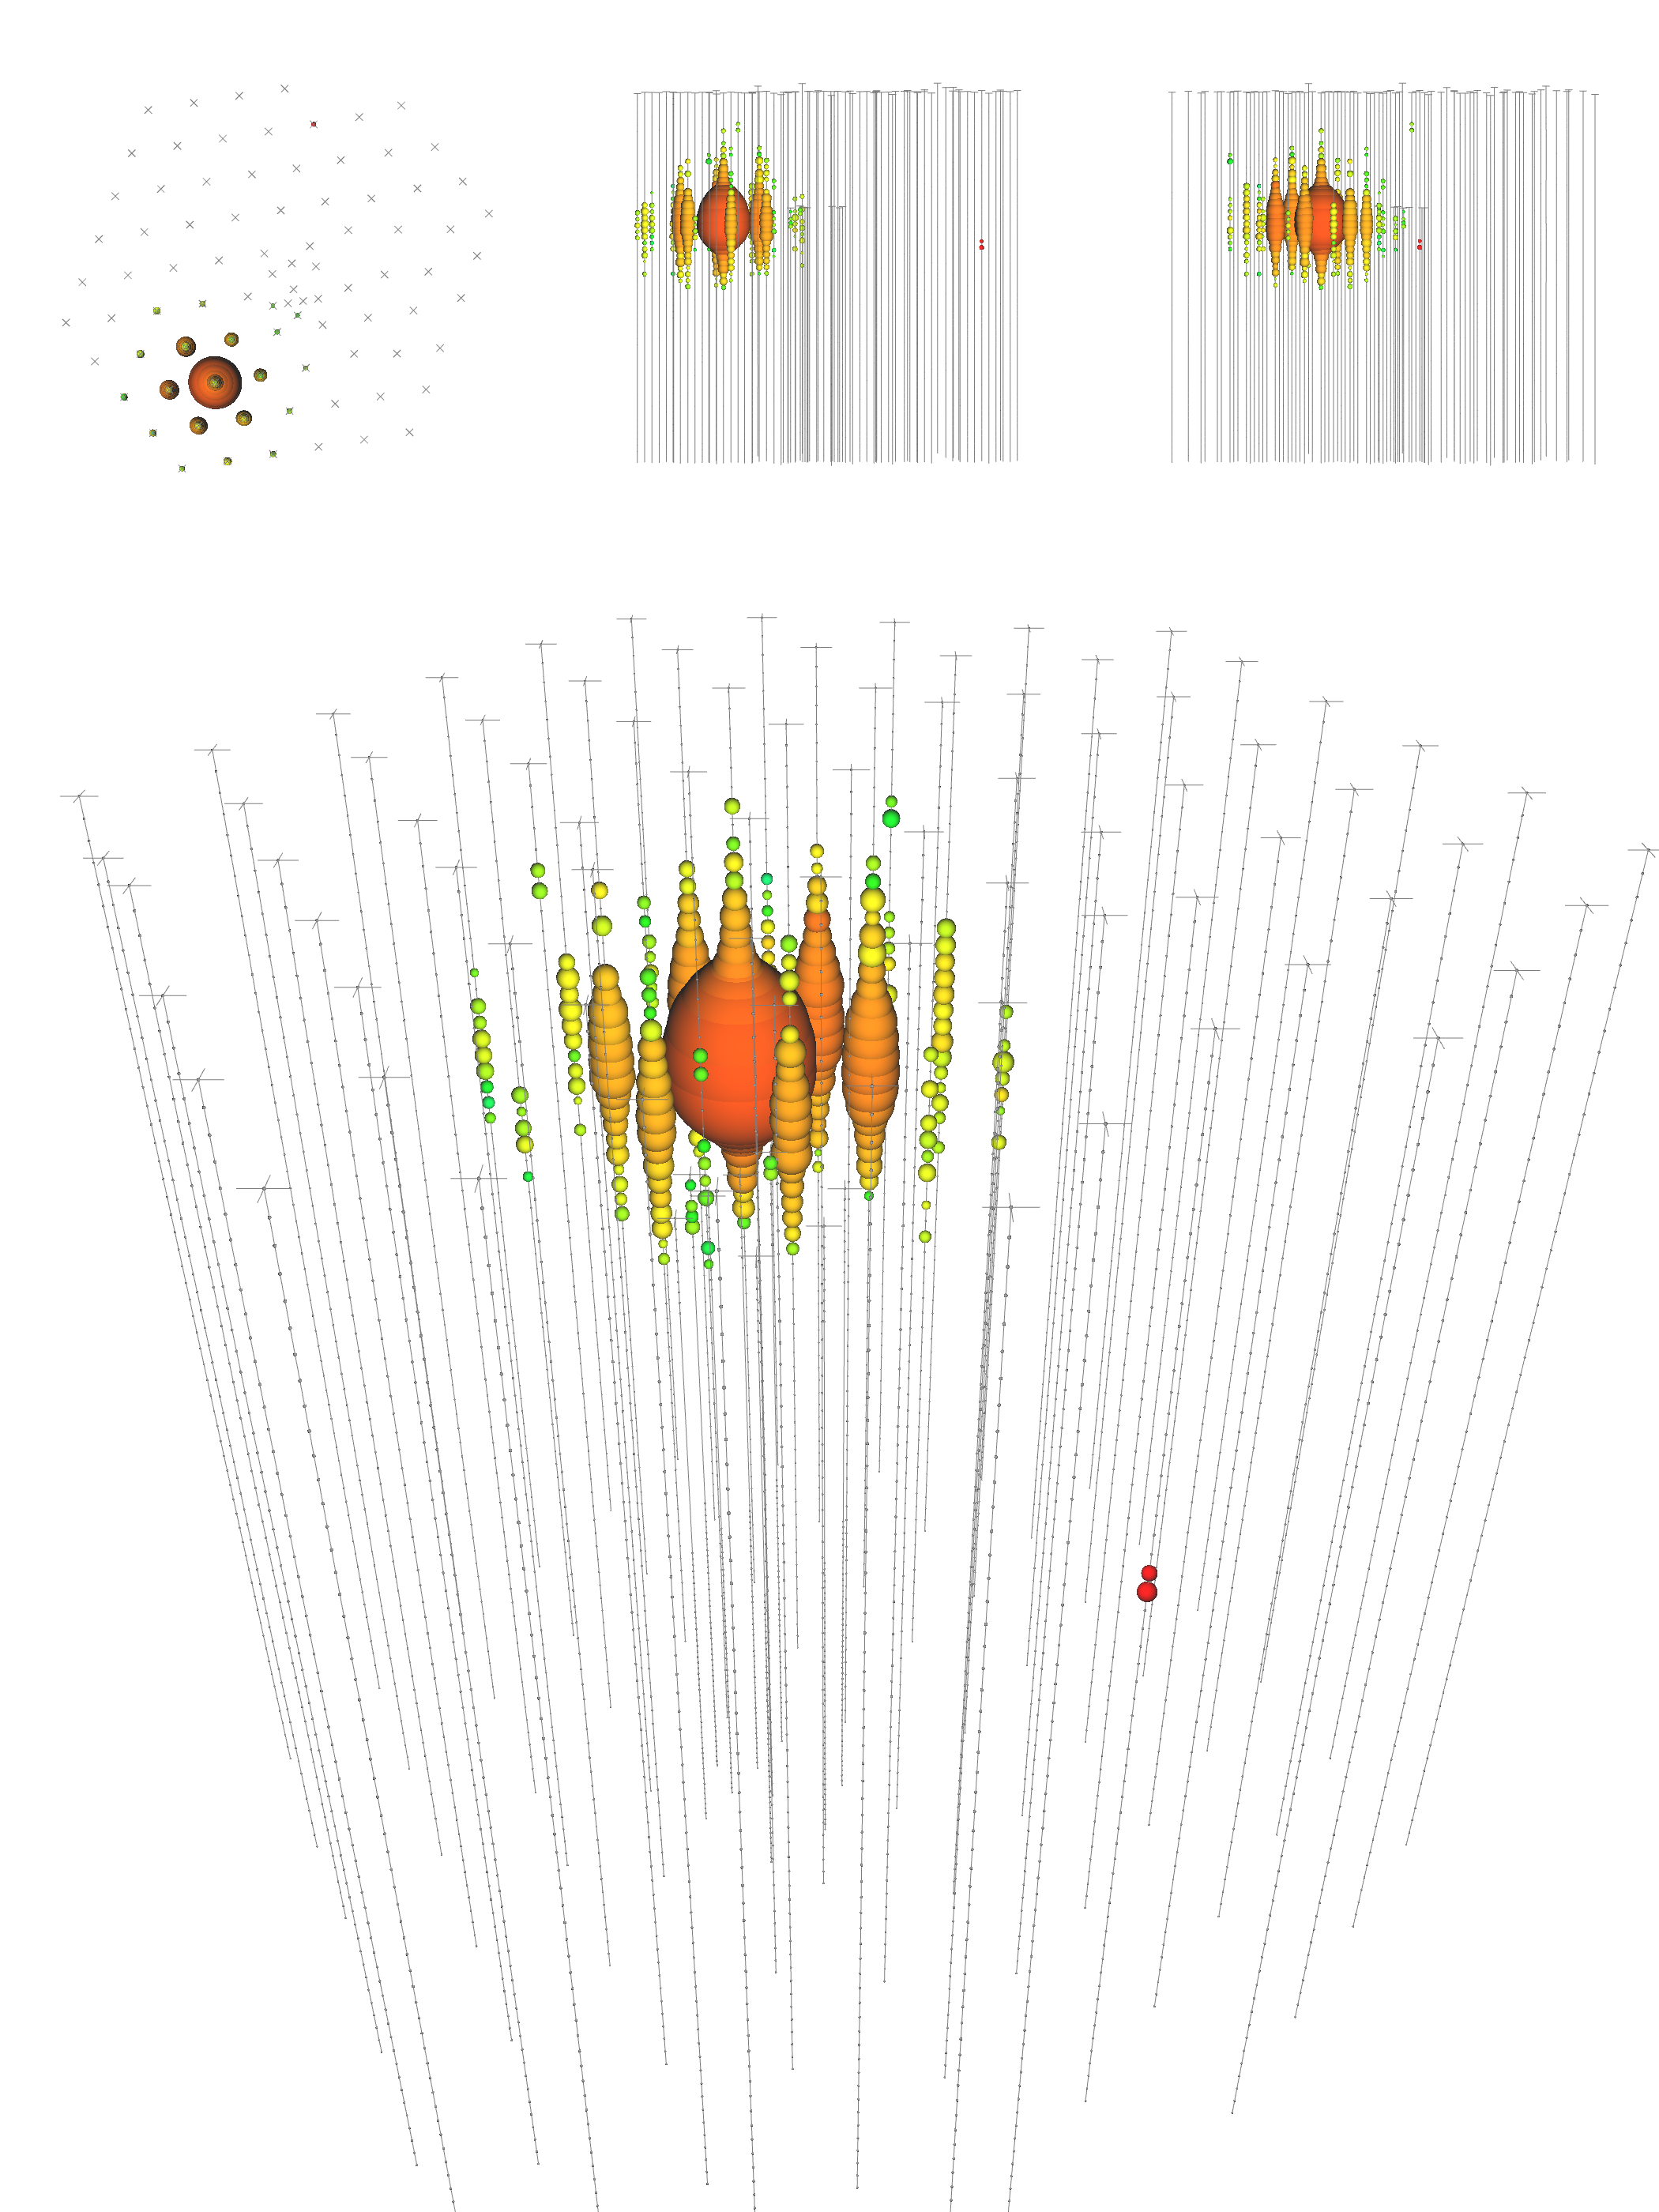
\includegraphics[width=1.0\textwidth,keepaspectratio]{hese_cascade_event.png}
  \end{center}
  \caption{A high-energy cascade event in IceCube with deposited energy of $210\pm^{29.0}_{25.8}$ TeV \cite{2013Sci...342E...1I}. The colored spheres represent DOMs that have registered light during the event. The size of the spheres are indicative of the total light received by the PMT on that DOM. The color denotes the timing of the hit with red corresponding to earlier times and blue corresponding to later times.}
  \label{fig:cascade}
\end{figure}

Whereas the resultant hit pattern for NC interactions is flavor independent, the event topology in CC interactions is determined primarily by the lepton flavor of the neutrino. In addition to a hadronic cascade, the CC interaction will also yield an energetic lepton corresponding to the flavor of the interacting neutrino. In the case of $\nu_{e}$ and $\nu_{\tau}$ CC interactions, the resulting hit pattern in IceCube will take the form of a cascade in a similar manner to the NC interactions. While the source of Cherenkov emission is no longer point-like, the length of electron and tau particle tracks is much shorter than the inter-DOM separation distance. Some marginal pointing can be achieved for these events, however, since the light produced in the hadronic and electromangetic cascades in these events is not totally symmetric. For sufficiently energetic $\nu_{\tau}$ events in IceCube, more exotic signatures are possible. These arise from the increased lifetime of the outgoing $\tau$ lepton resulting in two separate light-producing cascades that can be resolved separately either in space or time. As of the writing of this thesis, no events of this type have been observed in IceCube.

IceCube is designed specifically to be sensitive $\nu_{\mu}$ CC interactions due to superior pointing provided by long-lived muon tracks in the ice. Daughter muons from $\nu_{\mu}$ CC interactions can travel distances ranging from ~300 m ($E_{\nu_{\mu}}\sim 100$ GeV) to several kilometers ($E_{\nu_{\mu}}\geq 1$ TeV) \cite{2001PhRvD..63i4020I}. As these muons travel through the ice, they produce light in electromagnetic showers through both ionization and stochastic radiation losses. Because the muon is traveling faster than the speed of light in the ice ($n_{ice} \sim 1.3$), the Cherenkov light generated about the muon track will form a cone which is ultimately aligned with the original neutrino direction. This results in a linear hit pattern in IceCube DOMs, providing a clear signal with good directional information. Muon tracks with the highest contained length in the detector provide the best resolution due to their long lever arm and low kinematic angular difference with respect to the parent neutrino. An example of a track event from a high-energy contained event search is shown in Figure \ref{fig:track}.

\begin{figure}[ht]
  \begin{center}
    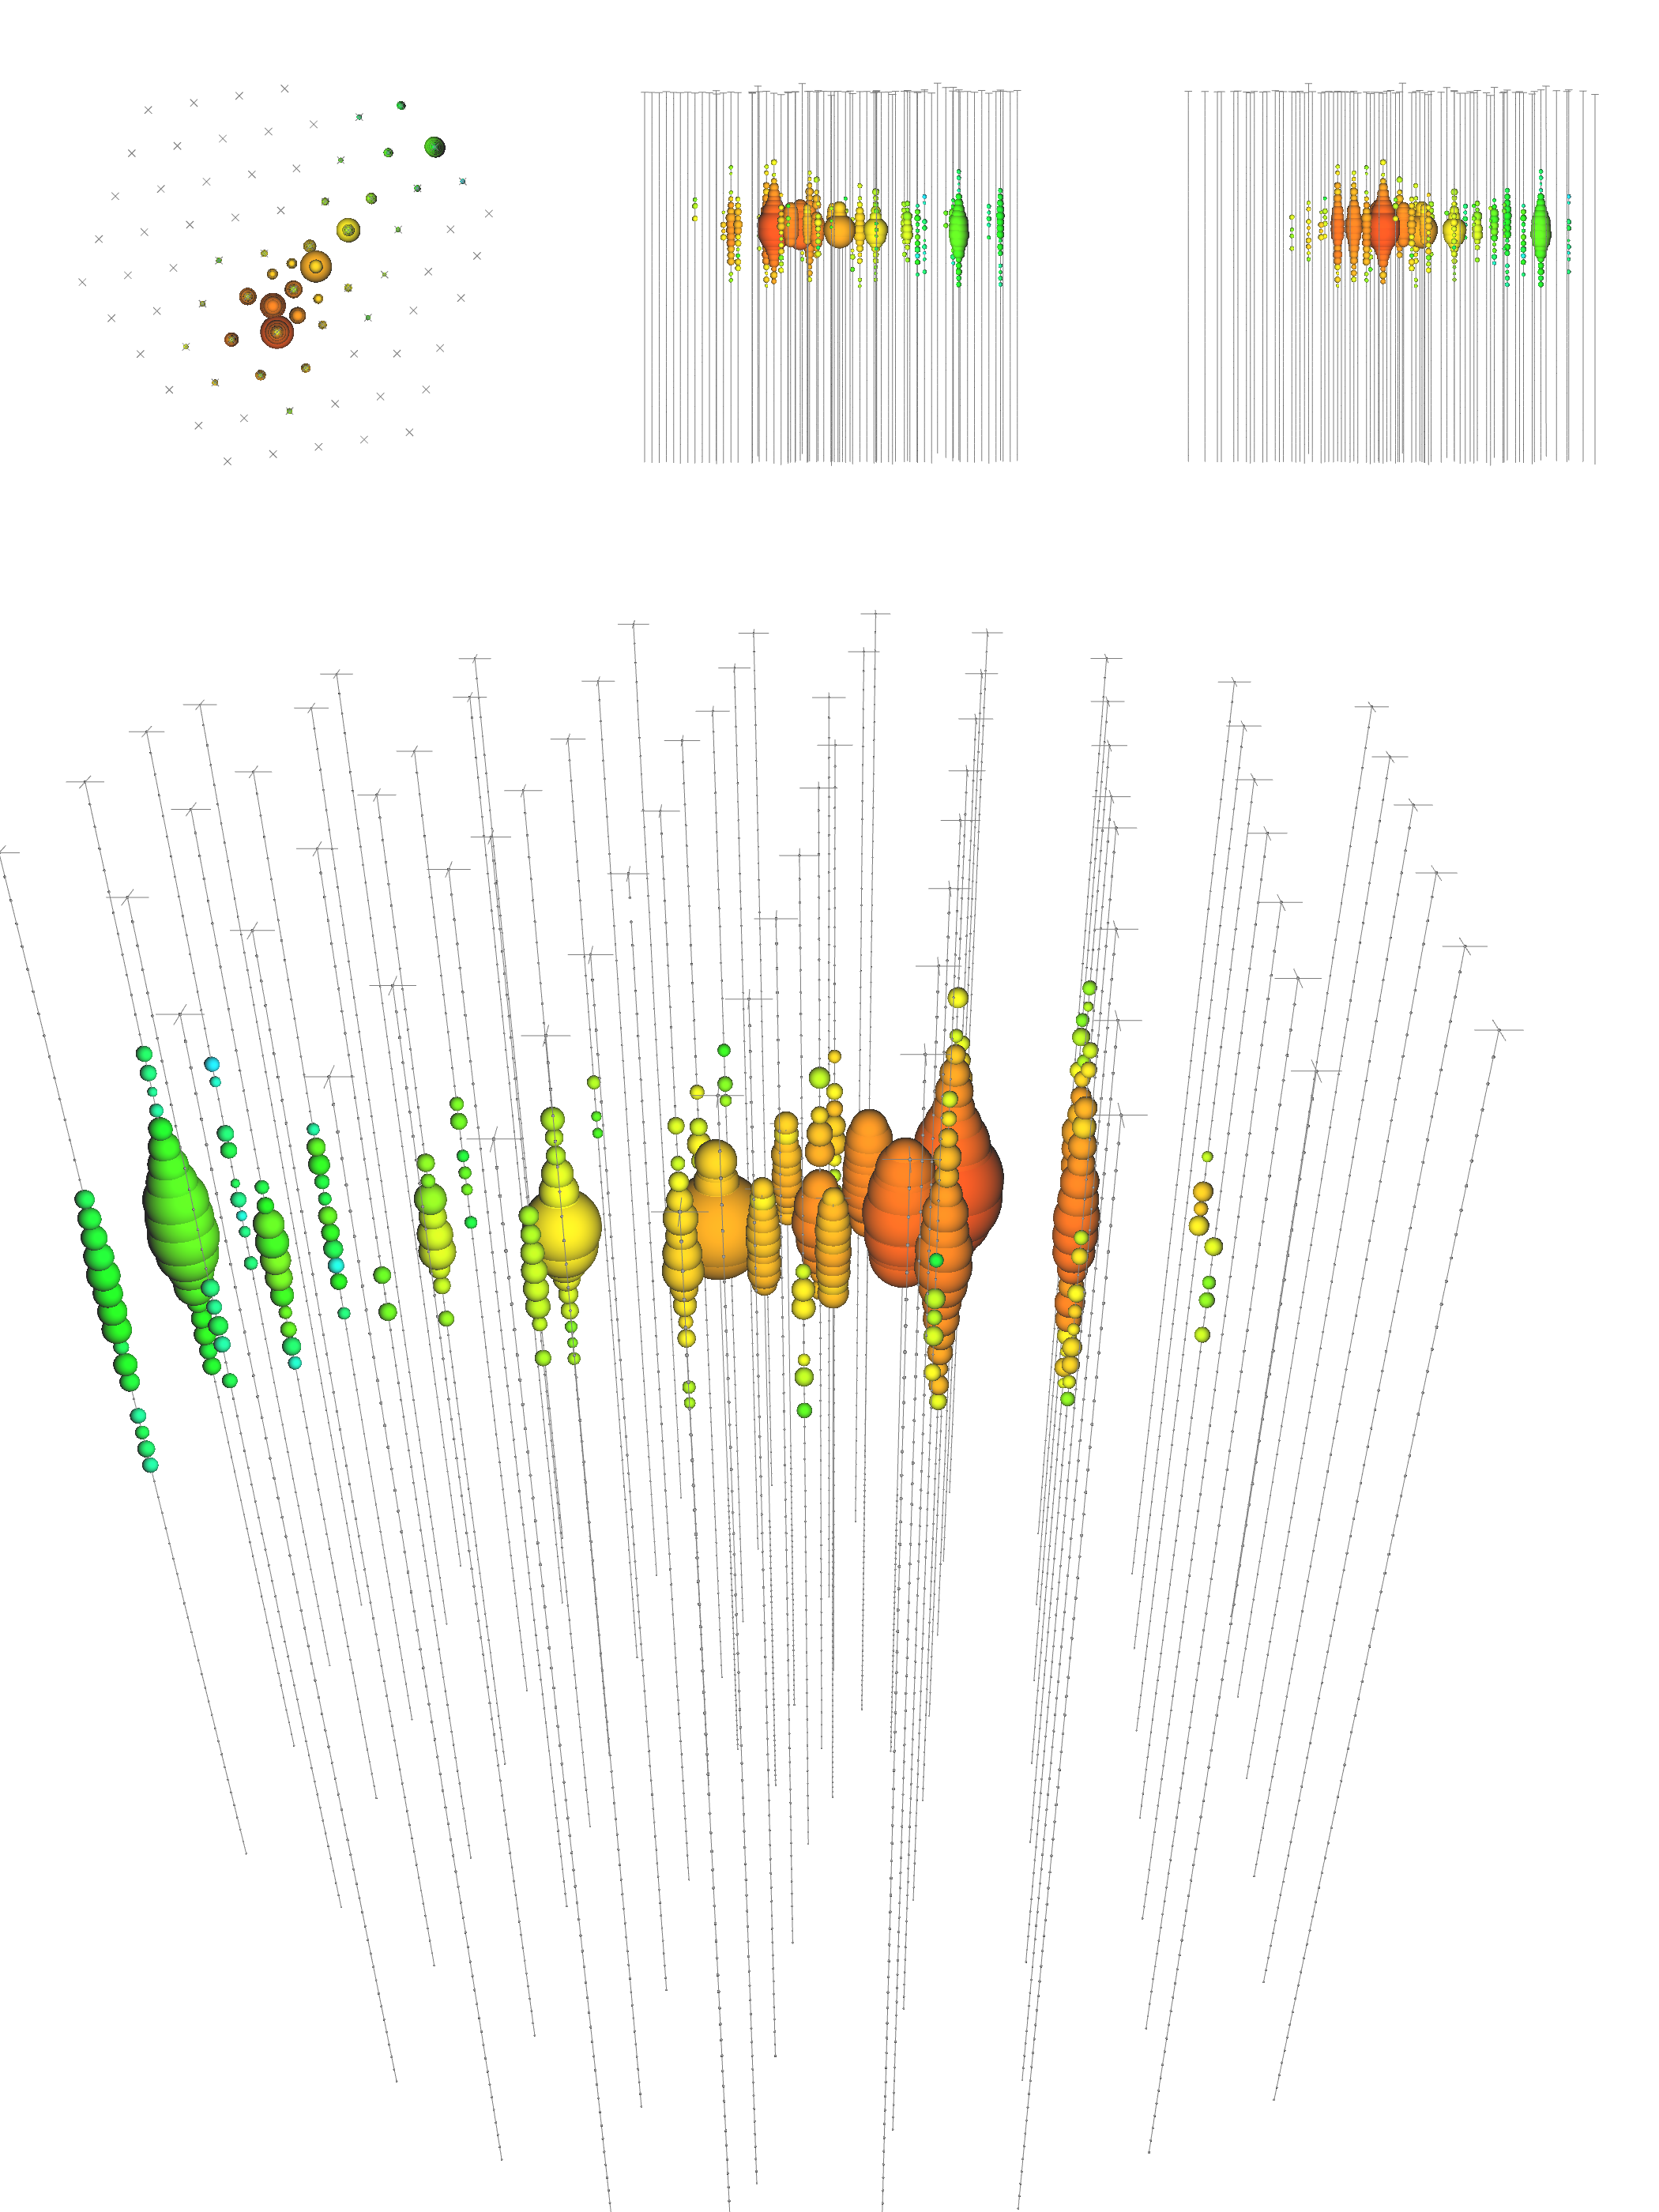
\includegraphics[width=1.0\textwidth,keepaspectratio]{hese_track_event.png}
  \end{center}
  \caption{A high-energy track event in IceCube with deposited energy of $71.4 \pm 9.0$ TeV \cite{2013Sci...342E...1I}. The colored spheres represent DOMs that have registered light during the event. The size of the spheres are indicative of the total light received by the PMT on that DOM. The color denotes the timing of the hit with red corresponding to earlier times and blue corresponding to later times.}
  \label{fig:track}
\end{figure}


\chapter{Data Acquisition}
Maintaining smooth and efficient data acquisition for a detector consisting of such a large number of sensors presents a formidable challenge. Reconstructing physics events within the detector requires accurate timing of signals received by individual sensors coupled with a high degree of synchronization among all detection elements. In this section, a succinct description of the detection of the light-yield from particle interactions in the ice and the subsequent processing of that data is given. The reader interested in a much more thorough account is encouraged to consult the summary by Abbasi et al. \cite{2009NIMPA.601..294A}. 

\section{The Digital Optical Module}
The essential component of the IceCube detector is the DOM. Each of these sensor units contains a Hamamatsu R7081-02 25 cm photo-multiplier tube (PMT), attached digitizing electronics, and LED flashers all housed within a glass pressure vessel \cite{2006NIMPA.567..214H}. A penetrator cable breaches the pressure vessel to connect the DOM electronics to the supporting string cable enabling DOM-to-DOM as well as DOM-to-surface communications. Figure \ref{fig:domscheme} provides an illustration of the DOM structure and its constituent components while Figure \ref{fig:dompic} gives a picture of a fully assembled DOM in its harness with breakout cable. Absolute quantum-efficiency measurements were made for all DOMs prior to deployment in the ice. In order to estimate how the efficiency might change after freeze-in, studies on the efficiency of DOMs at typical in-ice temperatures were performed in labs at IceCube member institutions. The inclusion of LED flashers at UV wavelength allows the DOM to simulate Cherenkov signals for the purpose of calibrating neighboring DOMs. These LEDs are also used to perform studies on the bulk ice properties near the DOM as well as the optical properties of the ice in the re-frozen water column in which the DOM is located.

\begin{figure}[ht]
\centering
\begin{minipage}[b]{0.45\linewidth}
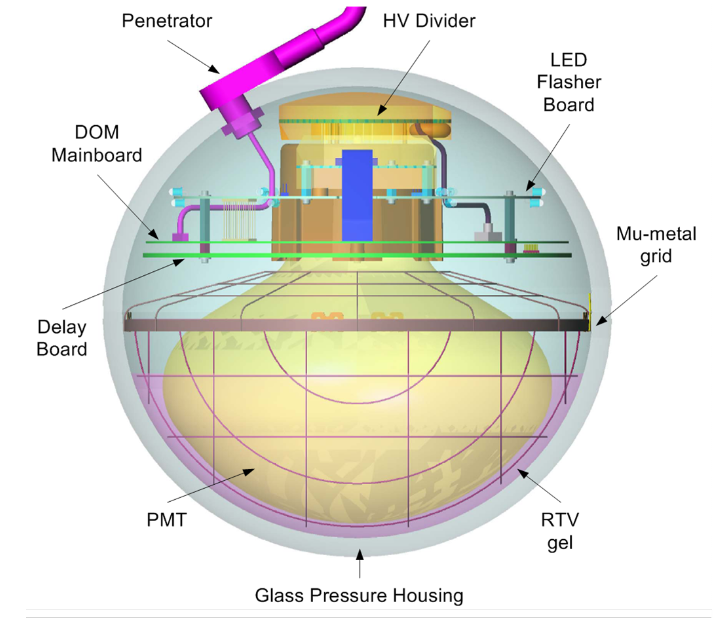
\includegraphics[width=0.95\textwidth]{DomSchematic.png}
\caption{Schematic detailing DOM structure \cite{2009NIMPA.601..294A}.}
\label{fig:domscheme}
\end{minipage}
\quad
\begin{minipage}[b]{0.45\linewidth}
\begin{center}
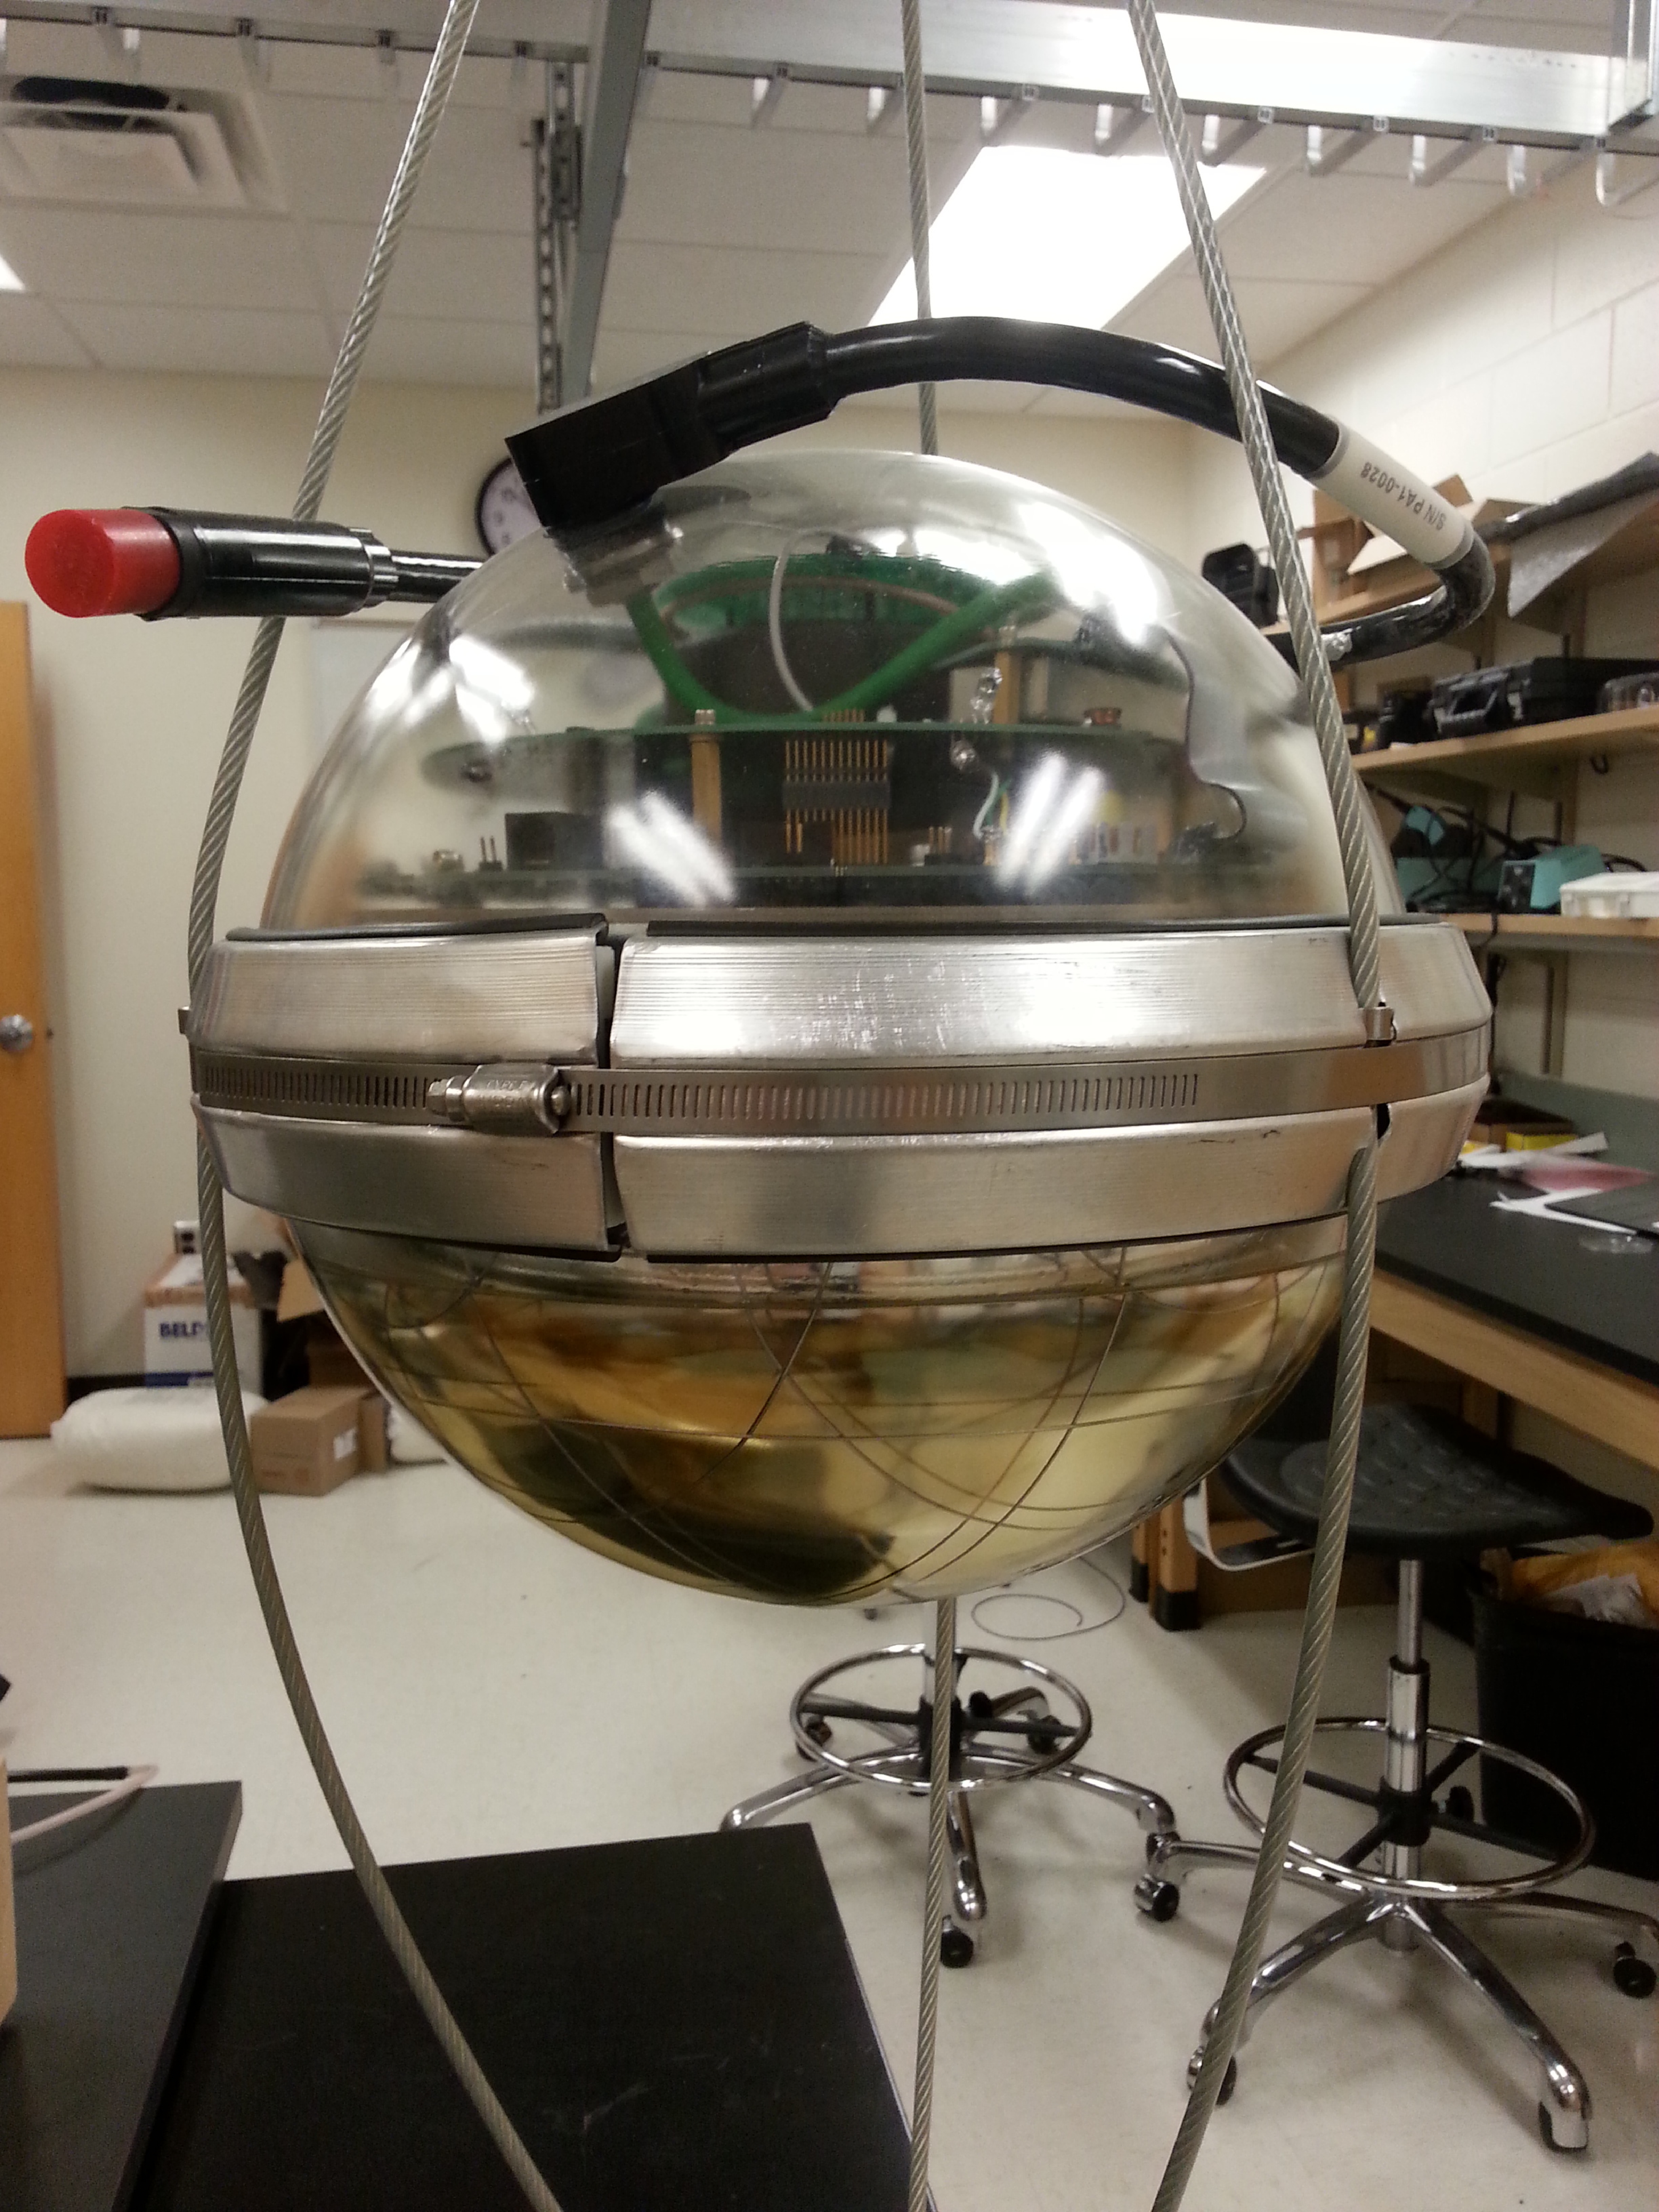
\includegraphics[width=0.75\textwidth]{LabDOM.pdf}
\end{center}
\caption{A fully assembled DOM supported by a cable harness.}
\label{fig:dompic}
\end{minipage}
\end{figure}

The operational lifetime of IceCube is tied directly to the survival of the DOMs in the ice. The inability to access these modules necessitated a design with a high probability of survival under intense pressures and cold operating temperatures. The design has so far proven to be quite robust; the DOM survival rate since first installation until the 2013-2014 season is an impressive 98\%. The majority of DOM failures occurred during the "freeze-in" period of their deployment where the pressures acting on the glass vessel are strongest \cite{2009NIMPA.601..294A}. These failures are likely the result of stress on the breakout cable and its connection. Very few DOMs have suffered from failure of main board electronics components meaning any DOMs that survive through freeze-in will likely have a long lifetime.

\section{Hit Generation}

All data acquisition begins with the registering and processing of photon hits in individual DOMs. The PMT of the DOM is configured so that the photocathode (which converts photons received by the PMT into electrons) is kept grounded while the anode is held at positive high-voltage.  Cherenkov photons from nearby passing charged secondaries are detected when they intercept the photocathode of the PMT on the underside of the DOM. This generates a small current pulse in the PMT which is subsequently amplified and sent to the main board of the DOM for digitization. After the pulse has been amplified, a local coincidence signal is sent from the DOM to its nearest and next nearest neighboring DOMs. In the event that a LC signal is then received from one of these neighboring DOMs, it is fed to an ATWD (Analog to Waveform Digitizer) which samples the input pulse 128 times at a rate of 40 Mhz. The capture and digitization process takes 29 $\mu$s, so the main board is equipped with two ATWDs that can run in parallel to minimize the amount of dead time in the DOM \cite{2009NIMPA.601..294A}. If the pulse received from the PMT is longer than the ATWD readout time, a ADC (Analog to Digital Converter) is also present to receive and digitize the signal. Additionally, pulses that fail to trigger LC with other DOMs will undergo digitization via the ADC rather than the ATWD. The pulses produced by the ADC have much coarser binning in time.

After digitization the pulses are sent to a FPGA (field-programmable gate array) which handles local coincidence triggering logic, generation of hits, and storing of hit information. This integrated circuit will readout the output from the digitizers and store the information until the hit information is ready to be communicated to the surface. Hits that satisfy the local coincidence criteria are known as HLC (hard local coincidence) while isolated hits that fail to show coincidence in other DOMs are referred to as SLC (soft local coincidence). The designation between HLC and SLC will determine how hits are handled further down the data processing pipeline. While some analyses prefer to work solely in the realm of HLC hit information to minimize the contribution of background effects, many reconstruction algorithms and low-energy analyses will favor the inclusion of SLC hits as they can represent true physics hits from a fainter source.

Collection of hit information from the DOMs is controlled by DOMHub computers located in the IceCube Laboratory (ICL) at the surface (see Figure \ref{fig:icl}). Each DOMHub machine is responsible for all 60 DOMs on a single IceCube string. The DOMHub computers are equipped with eight DOM readout (DOR) cards each of which is capable of handling communications with up to eight DOMs. The DOR cards signal the run state for the DOM, maintain time synchronization, send software updates, and monitors for any software or hardware failures \cite{2009NIMPA.601..294A}. The entire system is kept synchronized by a master clock updated by GPS and set to UTC. All of these components come together to ensure that all hit times measured by DOMs are reliable without any drift in relative time between separate DOMs or DOMHubs.



\begin{figure}[ht]
  \begin{center}
    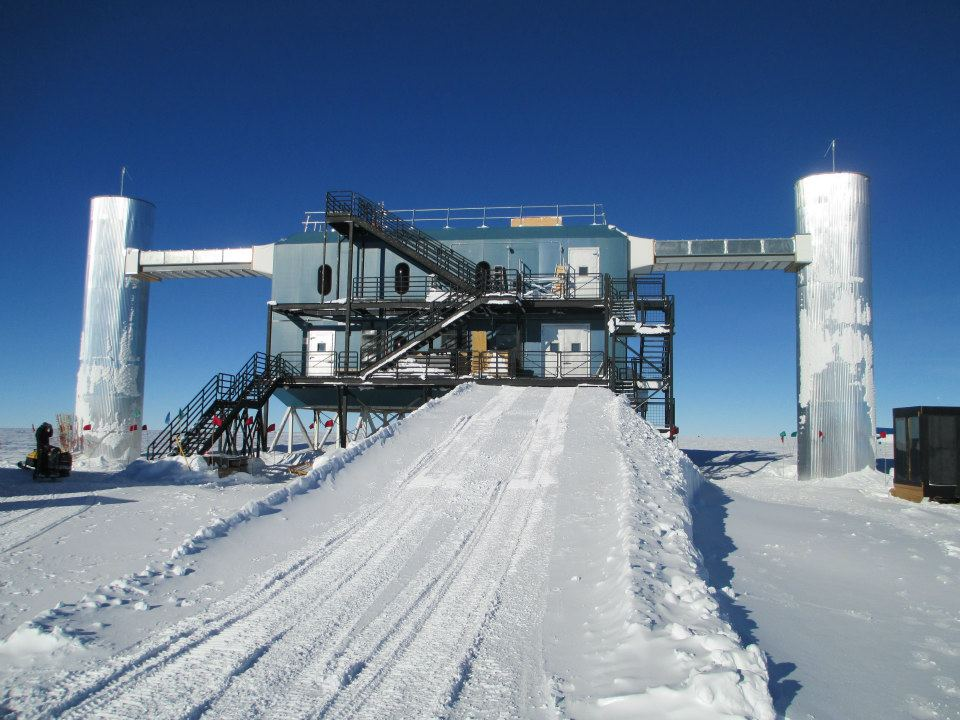
\includegraphics[width=1.0\textwidth,keepaspectratio]{ICL.jpg}
  \end{center}
  \caption{The IceCube Laboratory at South Pole. DOMHub computers located within the ICL communicate with all DOMs on a respective string. The cables carrying power and information for each DOM arrive at the ICL and enter the building from either the left or right tower near the ceiling (Photo credit: J. Daughhetee).}
  \label{fig:icl}
\end{figure}

\section{Triggering and Event Building}

The stream of DOM hit information arriving in the ICL must be parsed into physics events before any meaningful data analysis can be performed. During the average snapshot of the detector over a short time period ($\sim 10 \mu$s), there will typically only be DOM hits triggered by noise within the detector. In order to select out only interesting events, the IceCube data acquisition system (DAQ) examines the hit information continuously until a certain hit pattern 'triggers' the system to readout the data and construct a physics event. These triggers generally search for a clustering of events coincident in time that are consistent with a particle track or shower. Due to the diversity of analyses in IceCube, there are several triggers optimized for specific physics events. Only the three triggers taken as input for this analysis will be described, though. They can be summarized as follows:

\begin{adjustwidth}{2.5em}{2.5em}
\setlength{\parindent}{0pt}
\textbf{Simple Majority Trigger (8)} - This is the most commonly used trigger in IceCube analyses. This trigger requires that at least 8 DOMs record an HLC hit within a time window of 5 $\mu$s. When the trigger condition is reached, data during a time window defined by -4$\mu$s to +6$\mu$s with respect to the trigger firing time is readout by the DAQ and recorded as an event.

\textbf{Cylinder Trigger (4)} - Instead of solely using a multiplicity requirement, the cylinder trigger attempts to isolate events that show some clustering in space. It defines a cylinder about a DOM with a height of 75m and a radius of 175m. This cylinder encompasses a vertical section of five DOMs on the central string in addition to the nearest neighboring strings. The trigger condition is satisfied if there are 4 HLC hits within this defined volume in a time span of 1$\mu$s. The DAQ will then readout data from over a time window like that used for SMT8 events (-4$\mu$s,+6$\mu$s).

\textbf{DeepCore Simple Majority Trigger (3)} - This trigger works in a similar fashion to the SMT8 trigger. It has a much lower HLC hit threshold (3), but it only looks for HLC hits in DOMs below the dust layer on strings that comprise DeepCore. Additionaly, the time window is reduced from 5$\mu$s to only 2.5$\mu$s. The readout window for the DAQ is a bit larger than that for SMT8 (-6$\mu$s,6$\mu$s). The high-quantum efficiency of PMTs in DeepCore DOMs combined with the lower HLC hit threshold result in far more noise-induced triggers than SMT8.
\end{adjustwidth}
\setlength{\parindent}{17.5pt}

The total trigger rate for the IceCube detector is about 9 kHz with the SMT8, DCSMT3, and Cylinder Triggers firing at inclusive rates of 2.3 kHz, 280 Hz, and 4 kHz respectively \cite{I3Live}. Many events will satisfy multiple triggers and/or the same trigger multiple times. The DAQ system will merge all concurrent satisfied triggers into a single event physics event which ultimately yields a triggered event rate of about 3 kHz \cite{I3Live}. This trigger rate produces an enormous volume of data of which only a small portion is transferred to the north via satellite. All triggered events are written to tape, however, and this data is eventually transferred from Antarctica to storage at the IceCube data warehouse. These physics events are the input for all IceCube analyses and the beginning of the analysis chain.

\chapter{Event Selection}
A quick comparison between the rate at which atmospheric neutrinos trigger the IceCube and DeepCore detectors ($\sim$ 10 mHz) and the overall event rate ($\sim 3$ kHz) readily shows that the data generated by IceCube is very strongly dominated by background. This background is almost entirely due to energetic muons produced in cosmic ray air showers passing through the detector from above. Due to the large range of physics capabilities of the detector, many different filters exist to reduce the data volume and select out events of interest to specific analyses. Event selection for IceCube analyses generally consists of selecting the appropriate filter(s) for the expected signal followed by application of several iterations of cuts optimized to reduce background to an acceptable level while maintaining efficiency with respect to signal events.

%% Simulation
Additionally, it should be noted that this particular low energy muon neutrino dataset produced by GENIE (\textbf{G}enerates \textbf{E}vents for \textbf{N}eutrino \textbf{I}nteraction \textbf{E}xperiments) makes some approximations in hadronic propagation and light yield that are known to not be correct.
\section{Low-energy Channel}

Because of the primary focus of this analysis on a lower-energy event selection, the DeepCore-dominated low-energy filter stream is taken as input. Selecting only events which pass this filter reduces the trigger-level data rate of 3 kHz to a much more manageable 37 Hz. The low-energy filter attempts to select a relatively background free sample by selecting a detection volume about DeepCore that does not extend to edge of the detector. This allows optical sensors outside of the detection volume to serve as dedicated downgoing muon detectors. Events that have hits on DOMs outside the defined detection volume that are causally correlated with the hits inside the volume are able to be identified as background muons. A schematic representation of this filtering algorithm is shown in Figure \ref{fig:DCVetoSketch}. 

\begin{figure}[ht]
  \begin{center}
    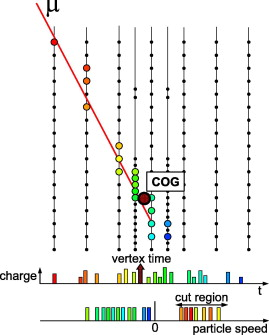
\includegraphics[width=.5\textwidth,keepaspectratio]{DeepCoreVeto.jpg}
  \end{center}
  \caption{Diagram of a downgoing muon traveling through IceCube into DeepCore. The colored circles indicate DOMs triggered by the muon with red representing earlier times and blue representing later times. The times of DOM hits in a defined veto region are compared to the time and location of the center of gravity (COG) fiducial volume DOM hits in DeepCore. Events that are found to have more than one veto region DOM hit causally correlated with the COG in DeepCore are filtered out as likely downgoing cosmic ray muons \cite{2012APh....35..615A}.}
  \label{fig:DCVetoSketch}
\end{figure}

This filter actually consists of two separate streams which are differentiated by the definition of which DOMs comprise the detection (or fiducial) volume and which DOMs are treated as belonging to the veto region. Inclusion of this additional branch using the relaxed veto allows for increased acceptance of higher-energy upgoing muon neutrino events that may be cut by the more stringent definition. The acceptance rate for the standard and relaxed veto filters is 17.25 Hz and 23.3 Hz respectively. The end result is a reduction in the trigger level data rate of nearly two orders of magnitude yielding a much more manageable data sample on which more advanced background reduction techniques can be applied.

\section{Analysis Specific Cuts}
After reducing the IceCube data stream to specific filters, the selection criteria imposed by differing will begin to diverge in order to optimize sensitivity to their respective target signal. For this analysis, the data given by the low-energy filter is put through a series of cuts optimized to preserve upgoing and contained track-like events from muon neutrino interactions. What event traits to cut on and to what degree was decided through examination of many cut choices on a sample of simulated muon neutrino events and background simulation. The end result is a selection of event cuts that can be grouped into two categories. The first category consists of cuts derived from detector information in the veto region while the second focuses on event quality and reconstruction characteristics. Lastly, a cut developed through machine learning techniques and optimized with respect to analysis sensitivity is applied to achieve a final level data set ready for analysis. The reader interested in a fully detailed description of the data selection process is encouraged to consult Appendix A.

\subsection{Veto Cuts}
Downgoing muons created in cosmic-ray air showers represent the most dominant background for muon neutrino analyses. As such, event selection processes go through extensive effort to identify and screen out these events.

\subsection{Quality Cuts}

\subsection{Machine Learning Cut}

%% Insert BDT Input Distributions


\section{Event Reconstruction}
An accurate reconstruction of neutrino events in the data sample is critical for optimal performance of any pointing analysis. During the event selection process several iterations of reconstructions are performed so that downgoing muons from cosmic rays can easily be identified. During data selection at lower levels, simpler reconstruction algorithms are often used to prevent a prohibitive amount of required CPU time for processing. These reconstructions then serve as the seed for more advanced techniques used at the analysis level. In this section the seed reconstructions for the final level will be discussed in addition to a detailed description of the final reconstruction whose results are used in the final analysis.

Reconstruction of a physics event within the IceCube detector depends on the geometry of the DOMs registering light from the event, the time of arrival for photons at those DOMs, and the total amount of light received at the individual DOMs.

%% Picture of Track event with reconstruction, PMT pulses

\begin{figure}[ht]
\centering
\begin{minipage}[b]{0.45\linewidth}
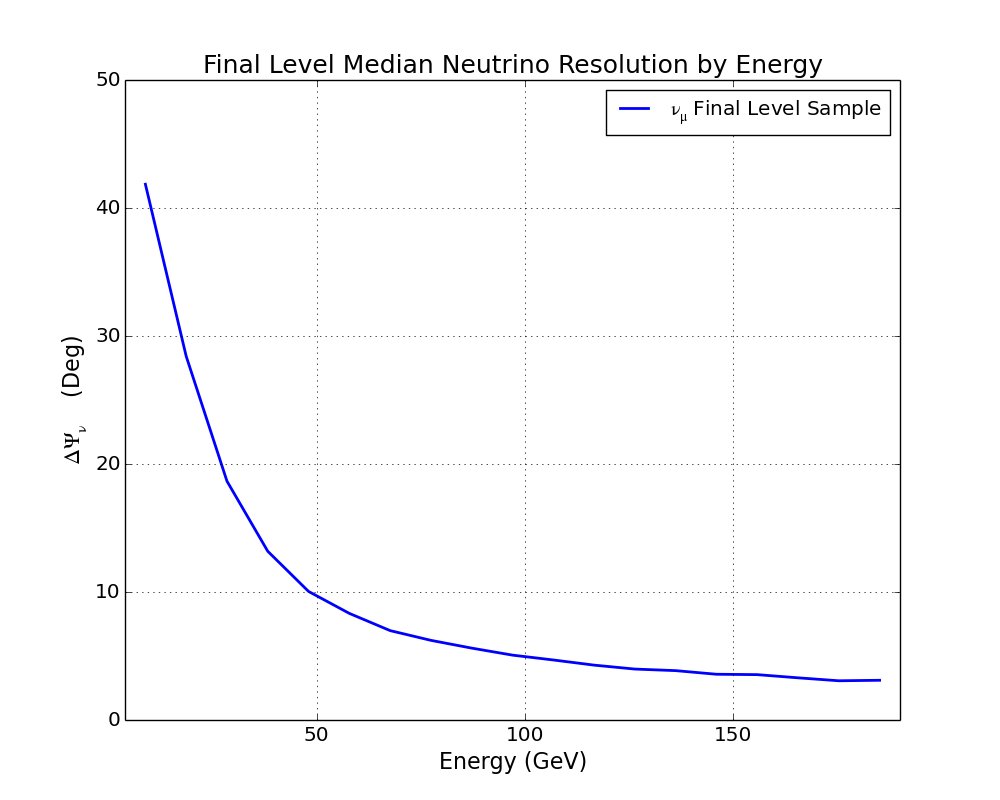
\includegraphics[width=0.95\textwidth]{FinalLevel_NeutrinoResolutionByEnergy_JustGENIE.png}
\caption{Median event resolution as a function of energy for simulation events passing all cuts.}
\label{fig:EventSampleRes_Energy}
\end{minipage}
\quad
\begin{minipage}[b]{0.45\linewidth}

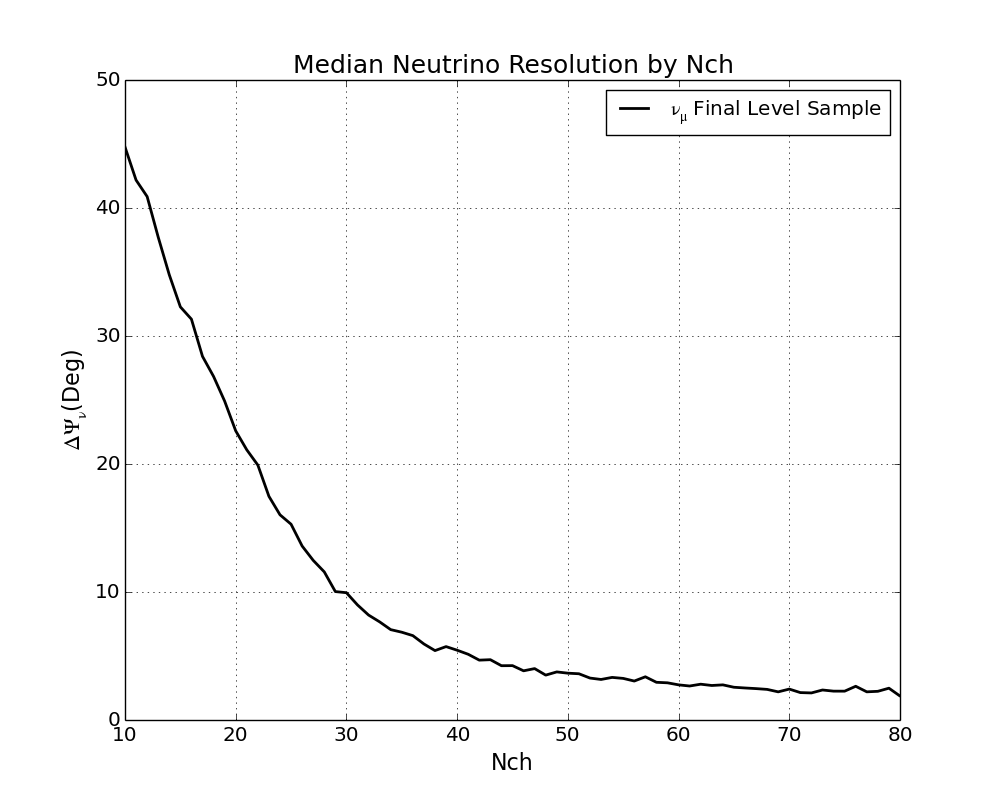
\includegraphics[width=0.95\textwidth]{GENIE_FinalLevel_NeutrinoResolutionByNch.png}

\caption{Median event resolution as a function of number of hit DOMs for simulation events passing all cuts.}
\label{fig:EventSampleRes_Nch}
\end{minipage}
\end{figure}

[Add Error Estimation from Paraboloid]


\section{Final Level Data}
After all cuts have been applied, we are left with a sample of 22,040 events during the observation period with an expected neutrino 'purity' of about 90$\%$. The bulk of these events are neutrinos of atmospheric origin and they represent an irreducible background for the analysis.
\begin{table}[h]
\caption[Final level data rate.]{Summary of event rates in mHz at each selection level. The amtospheric muon and neutrino rates are estimated through the use of Monte Carlo simulation (MC).\label{tab:event_rates}}
\begin{center}
\begin{tabular}{|l|r|r|r|}
  \hline
 \textbf{Event Type} &\textbf{ Cosmic Ray $\mu$} &\textbf{ Atmospheric $\nu_{\mu}$} &\textbf{ Collected Data}\\
\hline
Filter Level & ? & ? & ? \\ \hline
Level 3 & ? & ? & ? \\ \hline
Level 4 & ? & ? & ? \\ \hline
Level 5 & ? & ? & ? \\ \hline
\textbf{Final Level}     & \textbf{0.065 mHz} & \textbf{0.94 mHz} & \textbf{0.774 mHz} \\ \hline
\end{tabular}
\end{center}
\end{table}

%%% Insert Table for final level rates
%%% Refer to App. A for Pictures of Final Level Distributions
%%% Insert Effective Area Plot

\begin{figure}[ht]
  \begin{center}
    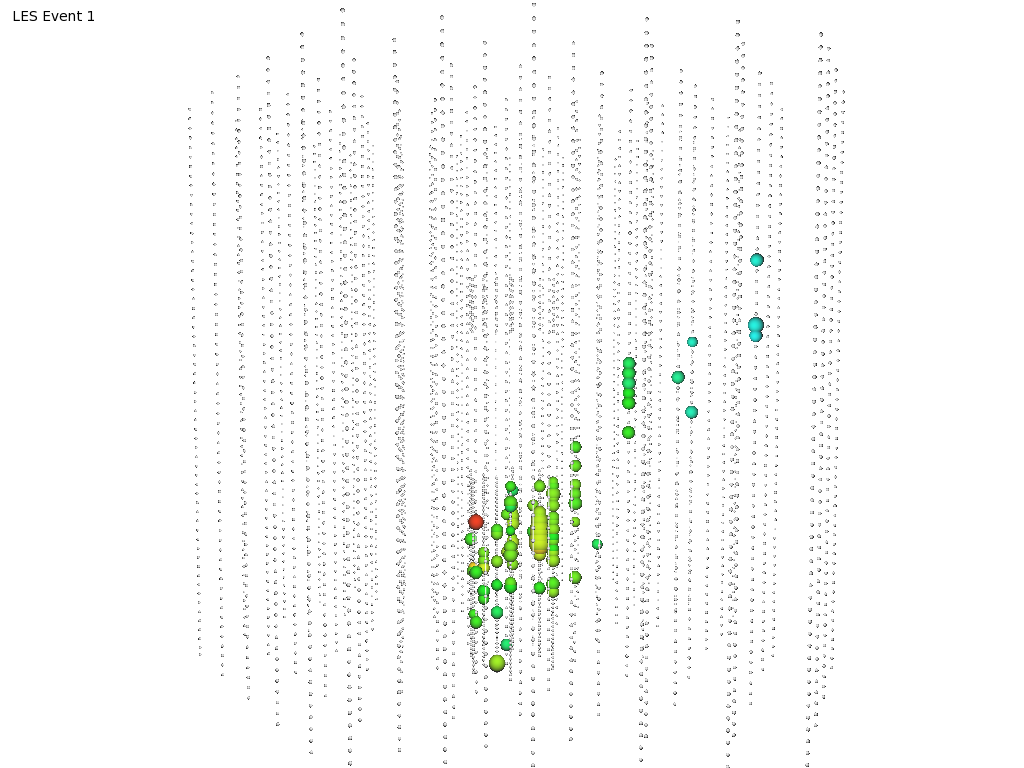
\includegraphics[width=1.0\textwidth,keepaspectratio]{LESEventForThesis.png}
  \end{center}
  \caption{Event display for a final level neutrino track event originating in DeepCore. The colored spheres represent DOMs that have registered a hit during the event. The size of the spheres are indicative of the total light received by the PMT on that DOM. The color denotes the timing of the hit with red corresponding to earlier times and blue corresponding to later times.}
  \label{fig:LESEventFinal}
\end{figure}


\chapter{Analysis Method}
%% Brief description of use of a time dependent search method
The analysis presented in this thesis makes use of both directional and timing information from the final level event dataset. The techniques that are used in this analysis have been applied to other IceCube event selections in a similar fashion. As of yet, these time-dependent searches focused on IceCube events have yet to find any time-dependent neutrino sources of significance higher than background expectations \cite{2012ApJ...744....1A}. A very thorough overview of the time-dependent likelihood analysis methods used in IceCube is given by Braun, et al. \cite{2010APh....33..175B}. The method detailed in the following section is mostly the same, but there are a few minor modifications made to the process to improve performance on a low energy event selection.


\section{Unbinned Likelihood Method}
The identification of a statistically significant astrophysical signal amongst a high number of background events can be a difficult problem in astronomy. Likelihood based methods are commonly used to solve this issue. Searches utilizing a likelihood method are able to provide a probabilistic interpretation of a signal hypothesis with respect to background fluctuations for the event dataset being examined. These searches will typically make use of timing, directional, and occasionally reconstructed energy information from events to find clustering indicative of a true astrophysical source. Whether or not individual events qualify as signal or background when testing a source hypothesis can differ depending on whether the search is 'binned' or 'unbinned'. For binned analyses, the signal hypothesis generates a set of coniditions that an event must meet to be considered as signal-like. This usually consists of selecting an area about the source location (a bin) that the reconstructed direction of the event must lie in. Events are then classified as either belonging to signal or being attributable to background. This results in all events having a binary status with respect to association with a hypothetical source. 

The unbinned method, which is the method chosen for this analysis, is typically more sensitive as it allows for events to be seen as both signal or background. In order to accomplish this, probability density functions (p.d.f.s) are constructed that are representative of the expected spatial, temporal, or energy distributions for both the signal and background possibilities. Thus, well-resolved events will strongly contribute to the likelihood calculation as signal- or background-like while more marginal events can make a contribution to either scenario with appropriate weighting instead of being sharply divided into either category. This makes the unbinned method much better suited for analysis of event samples with a wide range of resolutions.

The probability for seeing an event $i$ in our analysis given a time-dependent source hypothesis takes the following form:
\begin{equation}
\mathcal{P}_i(|\mathbf{x}_i-\mathbf{x}_s|,n_s,t_i,t_o,\sigma_w,\sigma_i) = \frac{n_s}{n_{\mathrm{tot}}} \mathcal{S}_i + \left(1-\frac{n_s}{n_{\mathrm{tot}}}\right) \mathcal{B}_i
\end{equation}
where $S_i$ and $B_i$ are the signal and background p.d.f.s respectively. The values of these PDFs depends on the reconstructed direction of the event \textbf{$x_i$}, the point spread function (PSF) of the event $\sigma_i$, the arrival time of the event $t_i$, the location of the hypothetical source \textbf{$x_s$}, the mean time of the flare $t_o$, the duration of the flare $\sigma_w$, and lastly the number of signal events $n_s$. The signal p.d.f. consists of both a spatial and temporal term. While the target sources for this analysis are expected to be point-like, the spatial term assumes a normalized extended distribution about \textbf{$x_s$} to account for the PSF of individual events $\sigma_i$. The signal p.d.f. is constructed in this way
\begin{equation}
\mathcal{S}_i(|\mathbf{x}_i-\mathbf{x}_s|,t_i,t_o,\sigma_w,\sigma_i) = S_i(|\mathbf{x}_i-\mathbf{x}_s|,\sigma_i) \cdot T_i(t_i,t_o,\sigma_w)
\end{equation}
\begin{equation}
S_i(|\mathbf{x}_i-\mathbf{x}_s|,t_i,t_o,\sigma_w) = \frac{\kappa}{4\pi \sinh \kappa} \exp \left(\kappa \cos |\mathbf{x}_i-\mathbf{x_s}|\right) \cdot \frac{1}{\sqrt{2\pi}\sigma_w} \exp \left(-\frac{(t_i-t_o)^2}{2 \sigma_w^2}\right)
\end{equation}
with the spatial term represented by the Kent-Fisher distribution \cite{1982} and the temporal term given by a Gaussian with mean time of $t_o$ and a width of $\sigma_w$. The concentration parameter $\kappa = \sigma_{i}^{-2}$ is determined by the event resolution. The inclusion of the Kent-Fisher distribution in the spatial p.d.f. represents a slight deviation from the standard construction of $S_i$ in IceCube analyses. It is analogous to the 2-dimensional Gaussian distribution on a flat surface, and for small values of $\sigma_{i}$ ($\lesssim 3^{\circ}$) the distributions are nearly identical. However, the Kent-Fisher distribution is properly normalized to the surface of a sphere. It therefore gives a better description of the spatial p.d.f. for events with larger uncertainties (which are common at the lower energies used in this analysis).
	
	The dataset being examined is heavily background dominated. This allows to simply derive our background p.d.f. directly from the final level dataset without having to make any assumptions about what the background should look like. Thus, the background p.d.f. will look like 
\begin{equation}
\mathcal{B}_i(\mathbf{x}_i,t_i) = P_{BkgDec}(\delta_i)\frac{P_{BkgAz}(\alpha_i)}{T}
\end{equation}
where $\delta_i$ and $\alpha_i$ are the event's reconstructed declination and detector azimuth respectively and $T$ is the total livetime of the analysis. By constructing the p.d.f. directly from the dataset we are able to fold in the declination dependence of both the muon and neutrino background as well as the difference in detector response. The IceCube detector is azimuthally symmetric, but the triangular lattice formed by its constituent strings do produce preferred corridors for background events to sneak through. This effect is fairly minor at the final event level, nonetheless it is also taken into consideration via the $P_{BkgAz}(\alpha_i)$ term. Lastly, the time dependence of the background is assumed to be flat. While there is seasonal variation in the atmospheric muon and neutrino rates, these modulations are not large at the final event level and the timescale of variation is much greater than the expected duration of neutrino emission from the target sources.

In order to find the best fit for the source parameters $n_s$, $t_o$, $\sigma_w$ at a specified location \textbf{$x_s$}, an optimizable likelihood function is needed. This function is given by the product sum of all individual event probabilities from the dataset:
\begin{equation}\label{eq:LLH}
\mathcal{L}(\mathbf{x}_s,n_s,t_o,\sigma_w) = \prod \mathcal{P}_i(|\mathbf{x}_i-\mathbf{x}_s|,n_s,t_i,t_o,\sigma_w,\sigma_i)
\end{equation}
The value of this function will depend on all events within the dataset. Furthermore, we can maximize the ratio of the likelihood function with specific choices of signal terms to the value of the function under the null hypothesis ($n_s=0$) to yield a best fit to the data. The value of the likelihood ratio yields a test statistic $\lambda$ given by
\begin{equation}
\lambda = -2\log \left[\frac{\mathcal{L}(\mathbf{x}_s,n_s,t_o,\sigma_w)}{\mathcal{L}(n_s = 0)} \right]
\end{equation}
with $\mathcal{L}(n_s = 0)$ being the null hypothesis and $\mathcal{L}(\mathbf{x}_s,n_s,t_o,\sigma_w)$ as the signal hypothesis being tested. Maximization of $\lambda$ through variation of the flare parameters yields
\begin{equation}
\hat{\lambda} = -2\log \left[\frac{\mathcal{L}(\mathbf{x}_s,\hat{n}_s,\hat{t}_o,\hat{\sigma}_w)}{\mathcal{L}(n_s = 0)} \right]
\end{equation}
where $\mathcal{L}(\mathbf{x}_s,\hat{n}_s,\hat{t}_o,\hat{\sigma}_w)$ are the optimized flare parameters. 

The test statistic is defined as such so that the distribution of $\lambda$ values from datasets consisting of only background events are well-modeled by a $\chi^2$ distribution with degrees of freedom equivalent to the number of parameters being fitted. Given that the background distribution is $\chi^2$ distributed, Wilks's theorem can be used to estimate the probability or p-value of seeing a clustering of neutrino events with test statistic $\lambda$ \cite{wilks1938}. This p-value allows the method to reliably identify the most statistically significant neutrino flare in the dataset.

While this formulation of $\lambda$ has been shown to yield a $\chi^2$ distribution of background test statistics for time-independent searches in IceCube, it does not produce a distribution similar to $\chi^2$ when used in time-dependent searches \cite{2012ApJ...744....1A}. This is due to a bias towards shorter flare duration in the analysis method. For a dataset of a given duration, it is possible to divide the data into many more short flare events than long flares. This creates an effective trials factor for shorter flares, and so the definition of the test statistic must be changed in order to compensate for this effect:
\begin{equation}
\hat{\lambda} = -2\log \left[\frac{\sqrt{2\pi}\hat{\sigma}_w}{T}\frac{\mathcal{L}(\mathbf{x}_s,\hat{n}_s,\hat{t}_o,\hat{\sigma}_w)}{\mathcal{L}(n_s = 0)} \right]
\end{equation}
The introduction of the marginalization factor $T/\sqrt{2\pi}\sigma$ brings the background $\lambda$ distribution back into agreement with the appropriate $\chi^2$ distribution \cite{2012ApJ...744....1A}.

To summarize, this analysis uses a likelihood ratio method to find the best values for a signal-plus-background model of the dataset. This is accomplished through maximization of ratio of the likelihood function with best fit parameters to the value of the function under the null hypothesis to generate a test statistic. The test statistic serves as figure of merit that characterizes the degree to which the data is better explained by a signal hypothesis rather than the background only scenario. Because we are not selecting any specific locations to test for flaring, the test statistic must be maximized at each possible location in the sky. The details of this process are described in the following section.
\section{Sky Scan}

The analysis performed is not a triggered search, and therefore it is necessary to examine the entire solid angle domain of the analysis for any possible transient sources. The difficulty in rejecting background muons at lower energies limits the analysis to up-going and horizontal events ($< 5^{\circ}$ above the horizon). Because of IceCube's location at the South Pole, this results in a search over all right ascension in a declination band ranging from -$5^{\circ}$ to $90^{\circ}$. The search method discretizes the northern portion of the sky into many bins, and the coordinates of these bins serve as the location of a hypothetical flaring source to be tested. The fairly large median resolution of the event sample (see Fig. \ref{fig:EventSampleRes_Energy}) allows the size of the search bins to be set to a relatively coarse 2$^{\circ}$ by 2$^{\circ}$ in angular area. 

Maximization of the likelihood given by eq. \eqref{eq:LLH} is done at each location in the grid with $\mathbf{x_s}$ set to the location of the bin. This results in each bin having a best-fit neutrino flare with its own values of $\hat{n_s}$, $\hat{t}_o$, $\hat{\sigma}_w$, and test statistic $TS$. After this scan over the 2$^{\circ}$ by 2$^{\circ}$ is completed, a finer follow-up scan with 0.5$^{\circ}$ by 0.5$^{\circ}$ binning is performed on any coarse bins with $-\log_{10}(p_{val}) > 1.75$ where $p_{val}$ is the estimated pre-trials p-value of the maximized test statistic. Following the completion of the fine-scan, the best-fit flare from the bin with the most significant test statistic is returned as the final result of the search. The results of a scan over a scrambled dataset consisting of only background events is shown in Figure \ref{fig:NullTrialSkyMap}.
\begin{figure}[ht]
  \begin{center}
    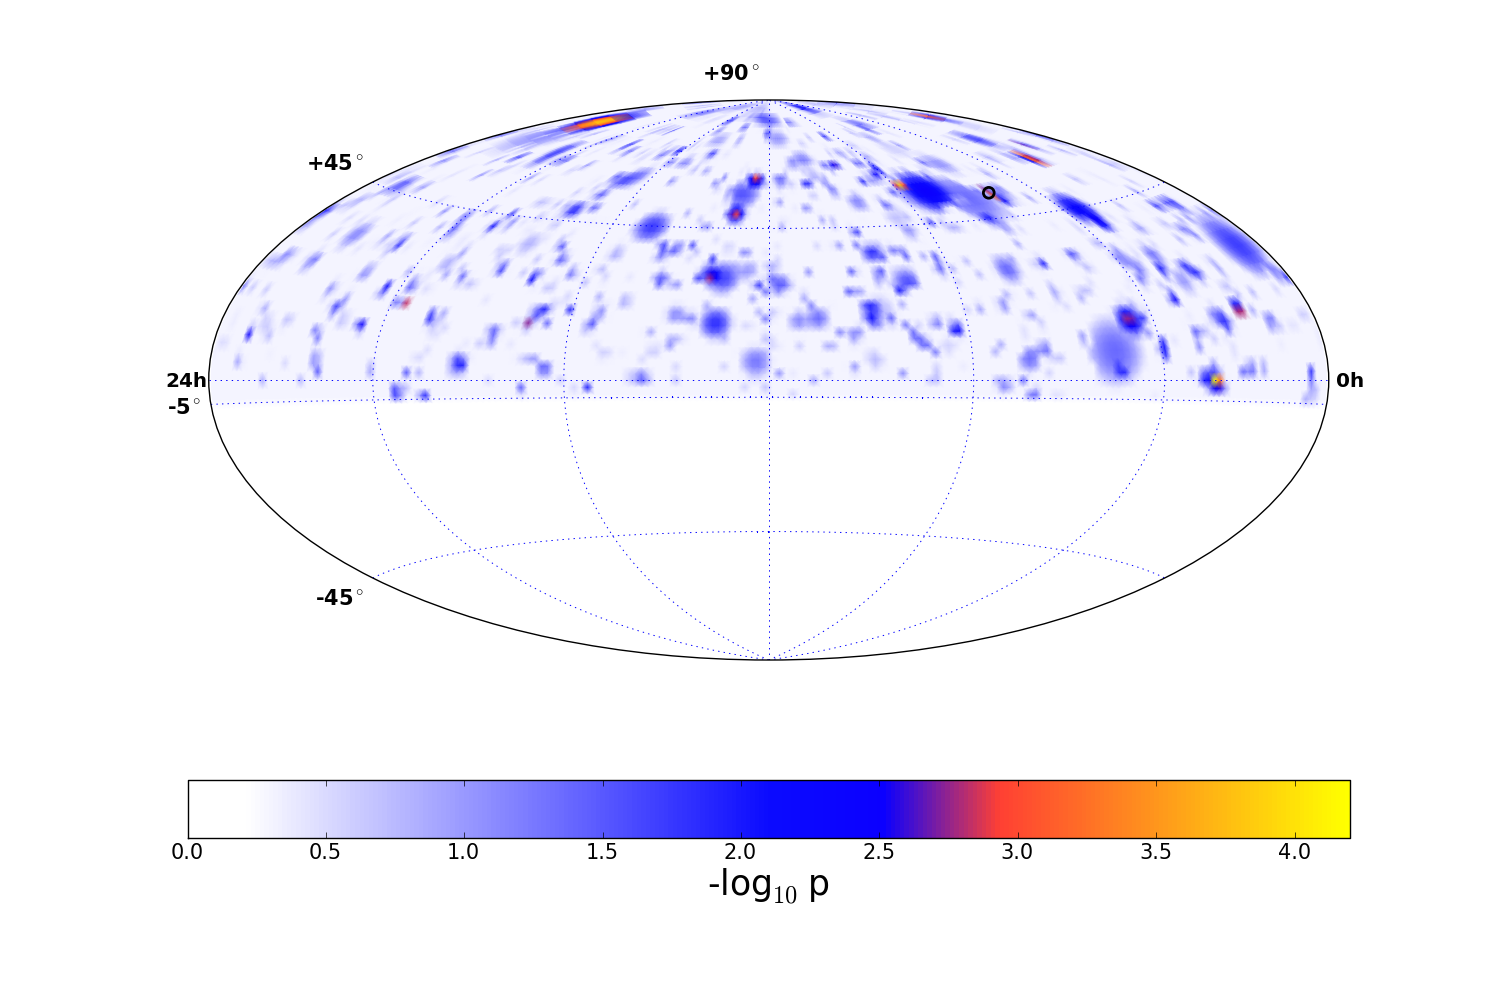
\includegraphics[width=1.0\textwidth,keepaspectratio]{NullMap996.png}
  \end{center}
  \caption{Sky map in celesital coordinates of pre-trials p-values for best-fit flares per bin for a randomized dataset. Random map generated by scrambling arrival times of real events. The black circle shows the location of the most significant flare found by the method. }
  \label{fig:NullTrialSkyMap}
\end{figure}

We calculate the sensitivity of this method by checking how well the search is able to pick out various levels of signal strength from background fluctuations. This procedure begins by selecting a point in the sky to perform our likelihood maximization. A background dataset is then generated by scrambling the time of arrival of the events. Due to the detector's location at the South Pole, this effectively scrambles the events in azimuth as well while keeping the declination distribution the same. The likelihood is then maximized for this set of scrambled data and the p-value obtained from the best fit is stored. This process is iterated many times to build a background p-value distribution. Injected signal events are now included in addition to the scrambled background data. Events are injected from an assumed source spectrum with a Poisson mean of $n_s$ that is increased until the desired fraction of p-values from signal injections (typically 90\%) beat the median p-value from the background only distribution. This is repeated for several different timescales in for a generic source with an $E^{-3}$ spectrum in Figure \ref{fig:SensE3}.
\begin{figure}[ht]
  \begin{center}
    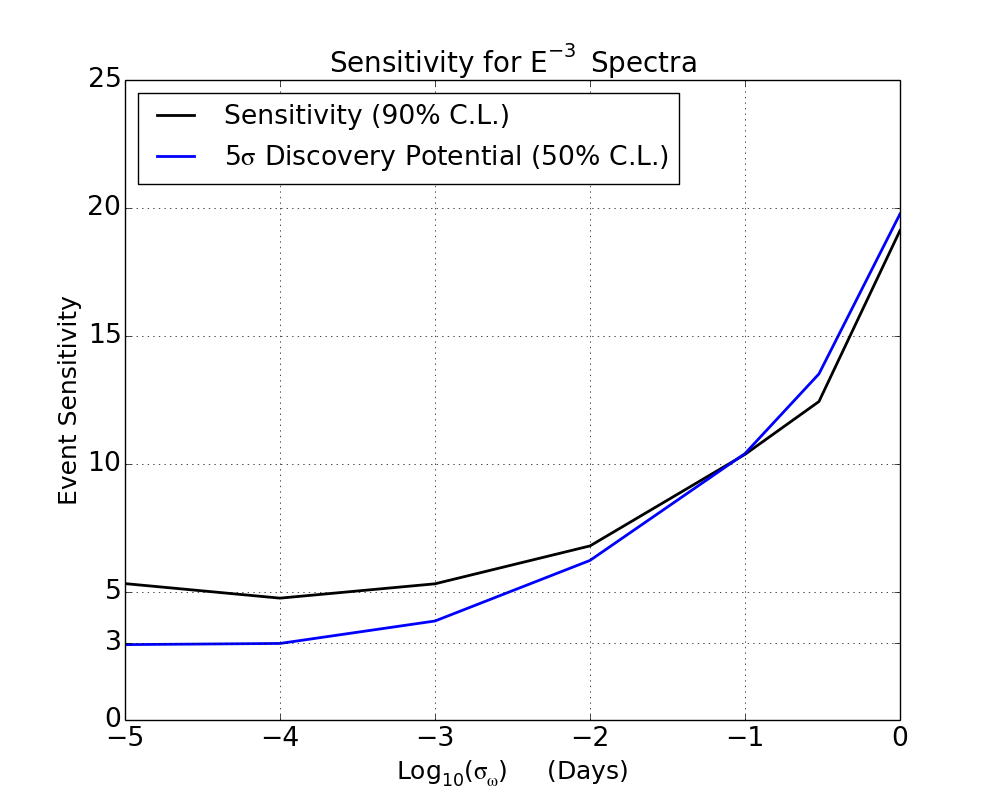
\includegraphics[width=.8\textwidth,keepaspectratio]{LowEnTransient_NEventDiscoveryPotentialANDSensitivity_E3.png}
  \end{center}
  \caption{Calculated event sensitivity of the analysis at Declination $\delta$=$16^{\circ}$ for an $E^{-3}$ spectrum.}
  \label{fig:SensE3}
\end{figure}

The discovery potential (which is also plotted in Figure \ref{fig:SensE3}) is calculated in a similar fashion. Rather than building a background p-value distribution, a threshold p-value is chosen. In this case, the value is set to the probability equivalent to that of a one-sided 5$\sigma$ deviation. Injections are performed until the mean value of injected $n_s$ results in flares whose recovered p-value exceeds the threshold p-value 50\% of the time. This does not, however, take into account any trials factors that arise from performing the scan over the whole northern sky. It is clear that the sensitivity of this method will suffer greatly for flares of longer duration. This limits the application of the method to sources with duration of approximately $10^4$s or shorter. However, given that the analysis was developed with short transient sources such as core-collapse SNe ($\Delta T \sim 1-100s$), this degradation in performance at longer timescales should not be an issue.

\section{Significance and Trials Factors}
In order to determine which bin has the most significant flare, we evaluate an estimated p-value based on the maximized test statistic $\lambda$ for that bin. The distribution of test statistic values for individual bins is assumed to be $\chi^2$ distributed, however the test statistic distribution of best-fit flares for searches over background only datasets is not known \textit{a priori} however. Therefore it is necessary to perform many iterations of the analysis method using scrambled versions of the dataset to determine the distribution of the test statistic with no real signal present in the data. The desired level of statistical significance determines the number of trials required, e.g. determining what value of the test statistic constitutes a 3$\sigma$ outlier would require approximately $10^4$ scramblings. The background test statistic distribution for such scramblings $2\times 10^4$ is shown in \ref{fig:NullScramblingDistribution}.

\begin{figure}[ht]
  \begin{center}
    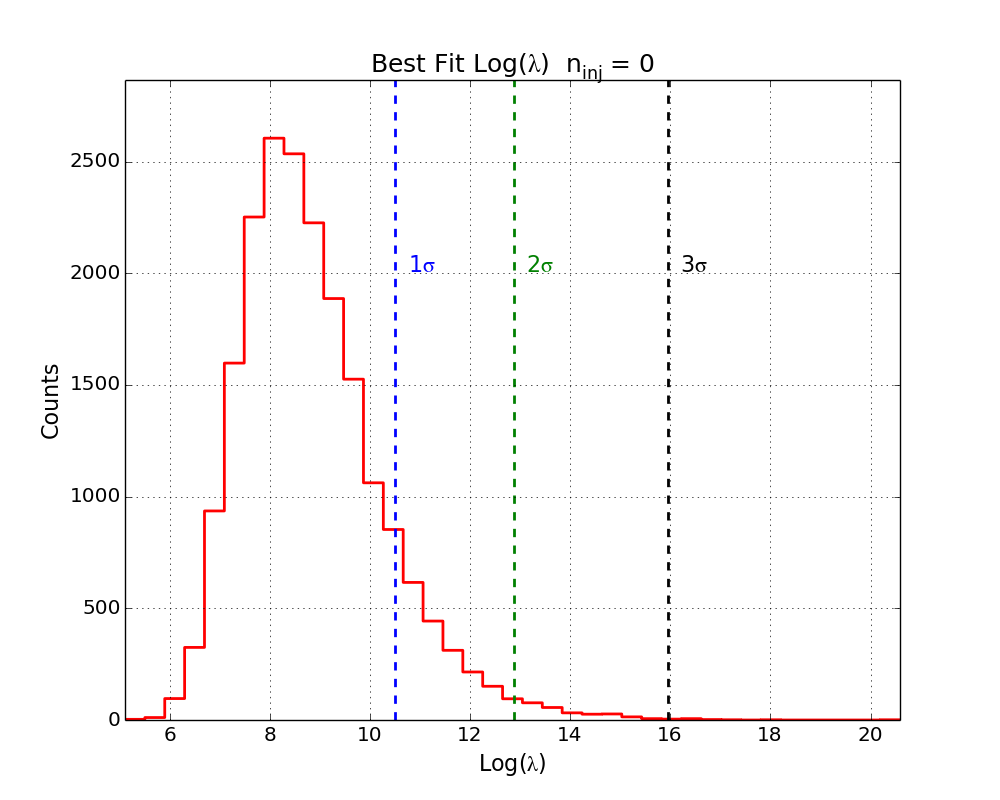
\includegraphics[width=0.98\textwidth,keepaspectratio]{TestStatisticDistribution_Null.png}
  \end{center}
  \caption{Distribution of maximized test statistic $\lambda$ for $2\times 10^4$ searches performed on randomized datasets. Dashed lines mark the location of one-sided $\sigma$ deviations.}
  \label{fig:NullScramblingDistribution}
\end{figure}

Once this distribution is adequately determined, the test statistic from any result we obtain from the analysis can be compared with the distribution we generated solely from background trials. This allows us to determine the probability of seeing a flare from just background fluctuations. This is sometimes referred to as the "p-value of the p-value" which is essentially the true p-value for the flare after properly accounting for all trials factors. This corrected p-value will be used when citing the significance of the final analysis result. 

The scrambled background trials also serve as a check for any biases in the analysis method with respect to best-fit parameters. The recovered flare parameters for these trials show no strong pull towards certain flare parameter values, though their is some mild declination dependence which is expected (the atmospheric background distribution is declination dependent). The distributions of best fit flare parameters for background trials can be seen in Figure \ref{fig:scramble_trials_parameters}. The symmetry of the detector is evident through the lack of preference in the azimuthal location of the best-fit flares. Additionally, the smooth distribution in recovered flare times reveals that the analysis method is able to avoid locking on to specific timescales.

\begin{figure}\label{fig:scramble_trials_parameters}
\centering
\subfigure[Right Acension]{\label{fig:a}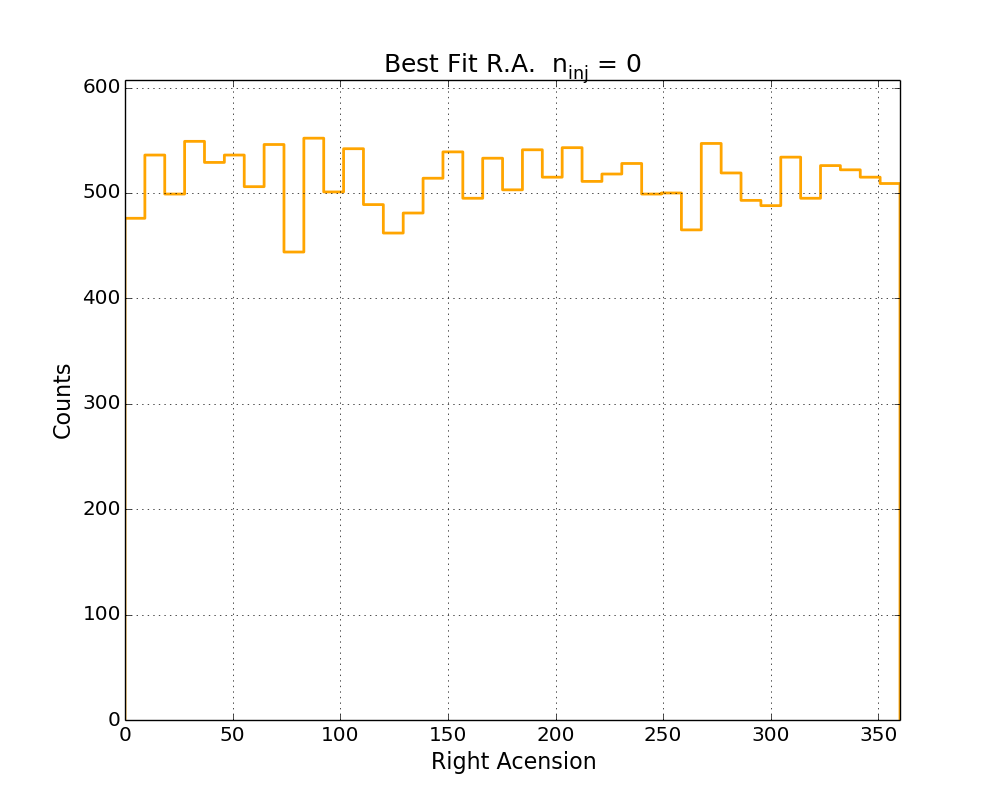
\includegraphics[width=70mm]{RightAcensionDistribution_Null.png}}
\subfigure[Declination]{\label{fig:b}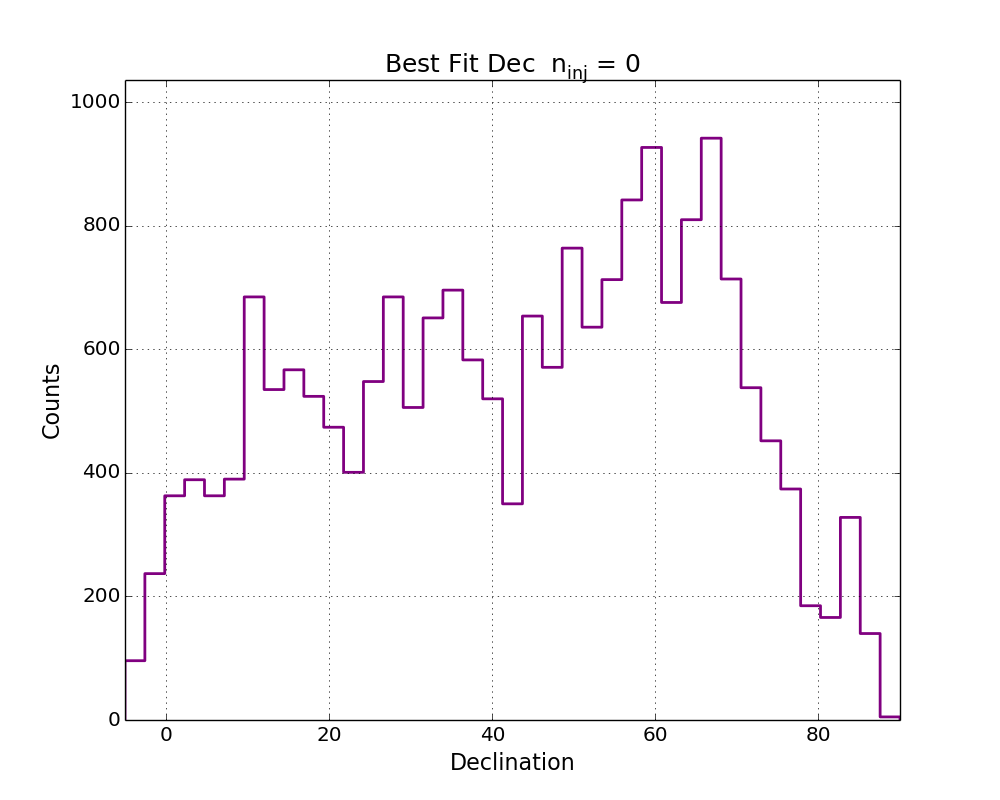
\includegraphics[width=70mm]{DeclinationDistribution_Null.png}}
\subfigure[Signal Strength $n_s$]{\label{fig:c}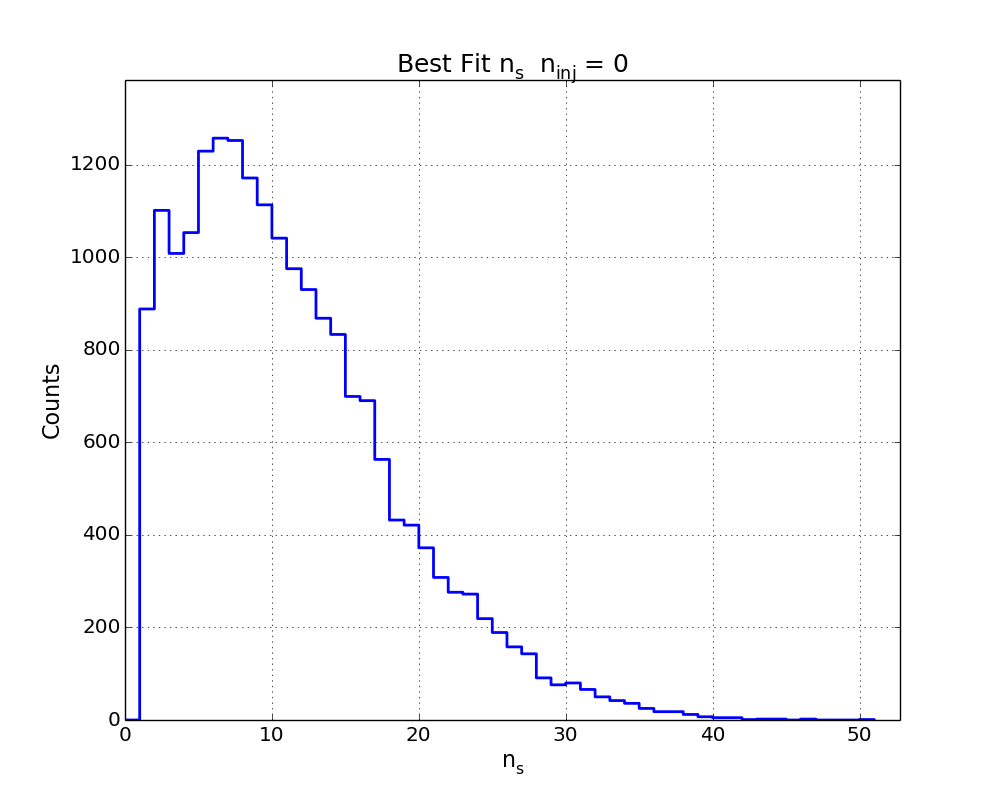
\includegraphics[width=70mm]{NSignalDistribution_Null.png}}
\subfigure[Flare Width $\sigma_w$]{\label{fig:d}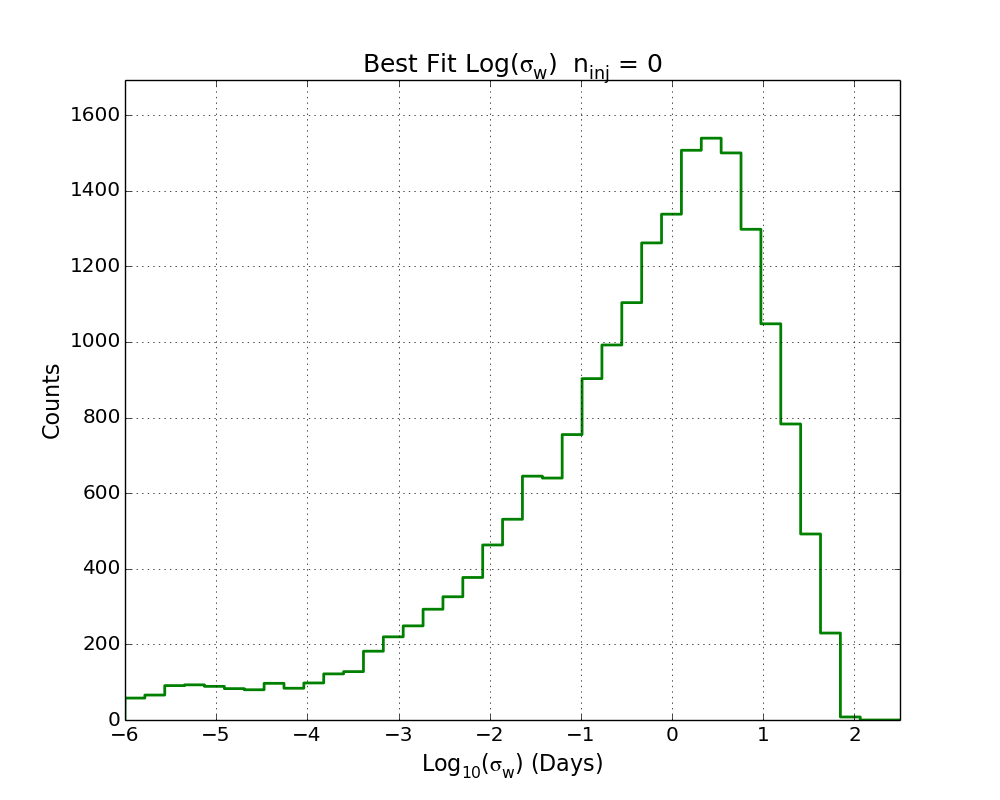
\includegraphics[width=70mm]{SigmaDistribution_Null.png}}
\caption{Distribution of flare parameters for the most significant flares identified by analysis method in $2\times 10^4$ trials on scrambled background-only data. The values plotted are the location of the flare in R.A. (a) and Declination (b). Also, the distribution of flare strengths measured in number of signal events is shown in (c) while the best fit flare duration is given by (d).} 
\end{figure}

\chapter{Systematic Effects}
There are many systematic uncertainties that can affect the interpretation of the results of this analysis. The primary contributors to uncertainty being the \textit{in situ} scattering and absorption properties of the ice medium and the absolute quantum efficiency of the PMTs within the DOMs. While there are other errors that could be considered such as the absolute neutrino cross-section, the contribution they provide to the overall error is negligible.

\section{Ice Properties}
The optical properties of the subsurface ice at the South Pole represent the most difficult systematic effect to adequately measure. This is largely due to the fact that this detection medium is inaccessible from the surface making direct measurement of the optical properties impossible. The scattering and absorption lengths in the ice greatly impact how light will propagate from interaction secondaries. Increased scattering can delay the arrival of photons to DOMs giving a larger spread in possible event interaction times. Assuming an incorrect absorption length can be problematic as well as it leads to inaccurate estimation of the total energy deposited by the neutrino event. If one hopes to reconstruct neutrino events with high enough accuracy for pointing, then it is necessary to develop a detailed and accurate model of the ice in which the detector is located.

Precise modeling of the polar ice is an ongoing task in the IceCube collaboration. Several iterations of models have reduced what was once a severe systematic problem to a relatively mild contribution to total systematic error. Current ice models consider several factors including depth dependence, tilt of ice layers, direction of glacial flow, and grain size distribution \cite{2013arXiv1301.5361I}. The absolute values of the optical properties such as absorption and scattering length are not known, however. Therefore we generate simulation that assumes different values for these parameters to estimate how large of an impact any error in the model will make at the final level of the analysis.

\begin{figure}[ht]
  \begin{center}
    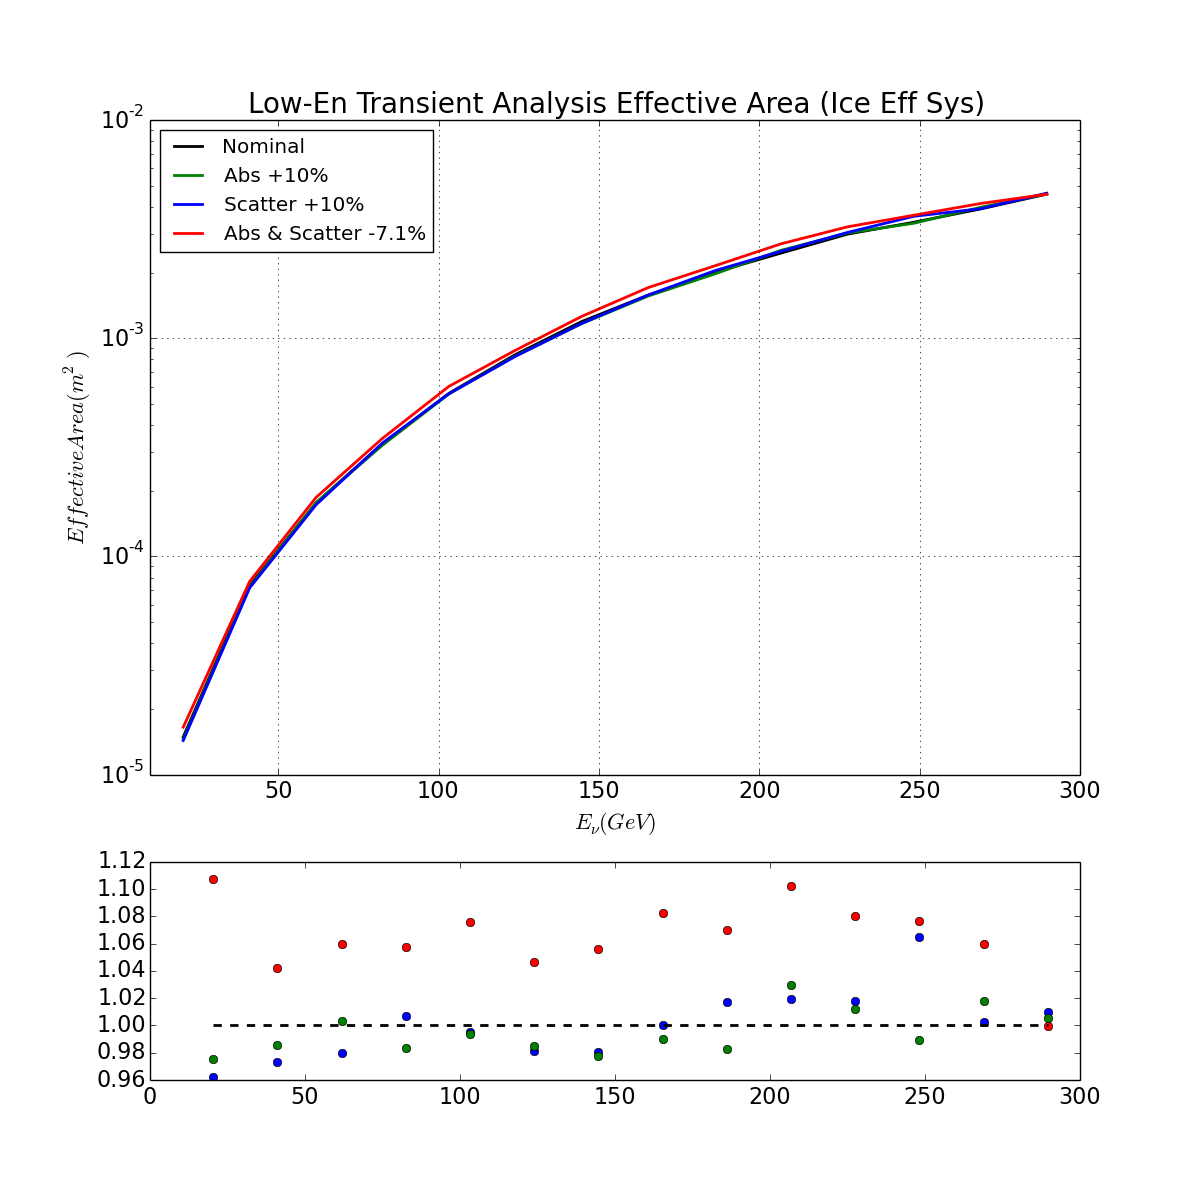
\includegraphics[width=0.98\textwidth,keepaspectratio]{LowEnTransient_EffArea_SysNugen_IceEffect_300GeVTrunc.png}
  \end{center}
  \caption{Effective area at final event level as a function of energy for different possible ice properties. Increased absorption and scattering lead to very little degradation of the neutrino effective area at even the lowest energies.}
  \label{fig:IceSysEffArea}
\end{figure}


\section{DOM Quantum Efficiency}

TBD

\begin{figure}[ht]
  \begin{center}
    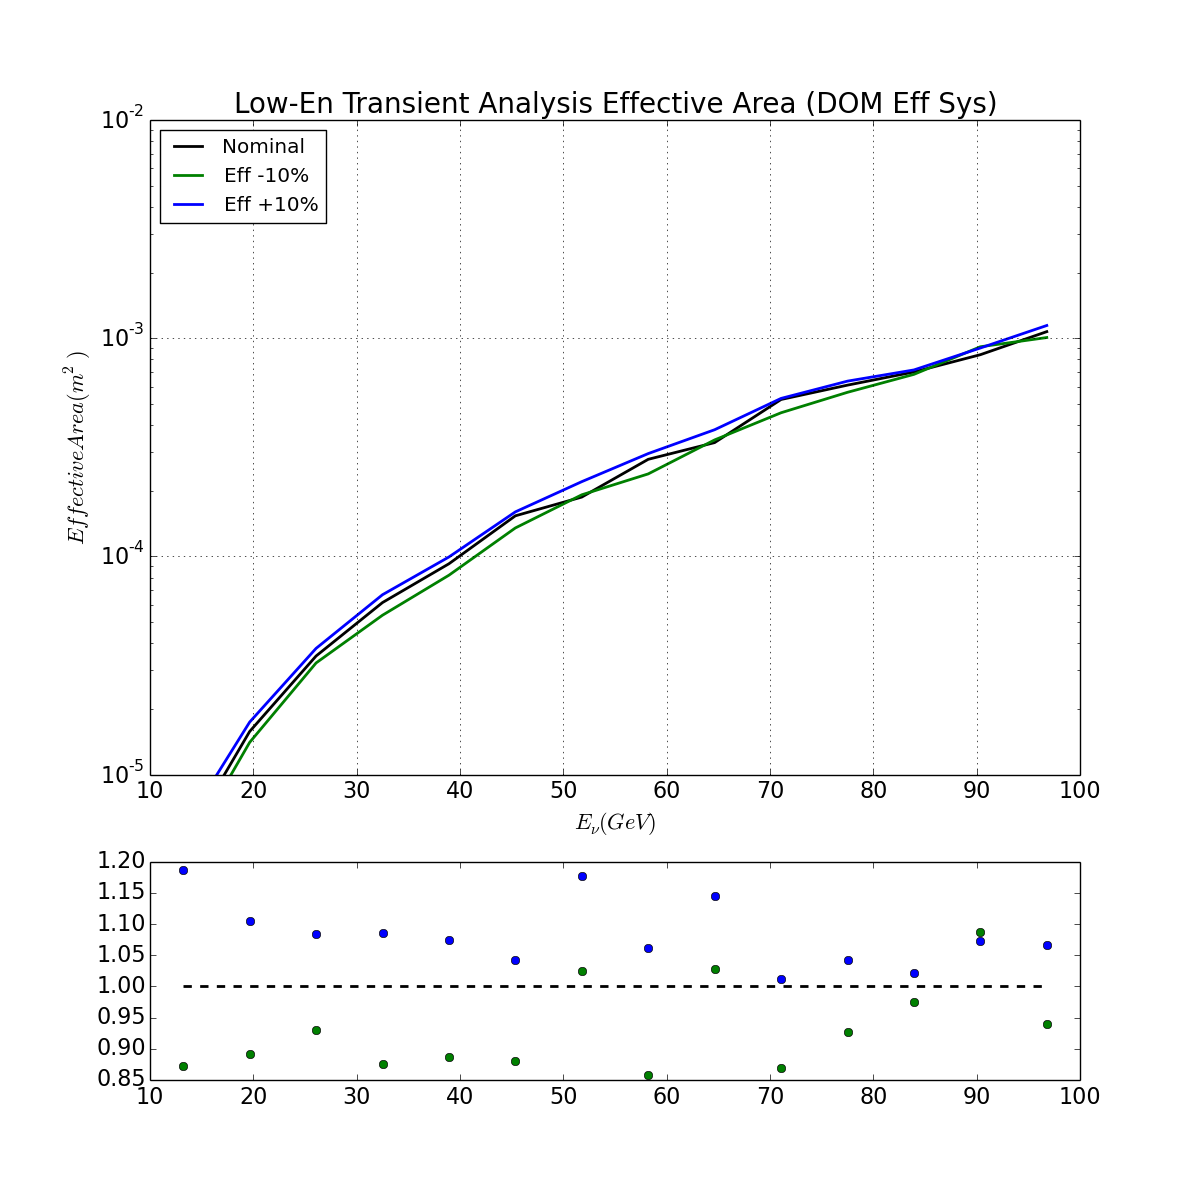
\includegraphics[width=0.98\textwidth,keepaspectratio]{LowEnTransient_EffArea_SysGENIE_DomEfficiency.png}
  \end{center}
  \caption{Effective area at final event level as a function of energy for different possible DOM efficiency settings. At lower energies, the change in effective area becomes approximately proportional to the relative change in DOM efficiency.}
  \label{fig:DOMSysEffArea}
\end{figure}

\chapter{Results and Interpretation}

\subsection{Search Result}
Applying the defined analysis method on the unscrambled dataset yields a skymap of the pre-trials p-values derived from the maximized test statistic for each bin (see Figure \ref{fig:RealSkyMap}).

%% Hottest Spot
%% SkyMap
\begin{figure}[ht]
  \begin{center}
    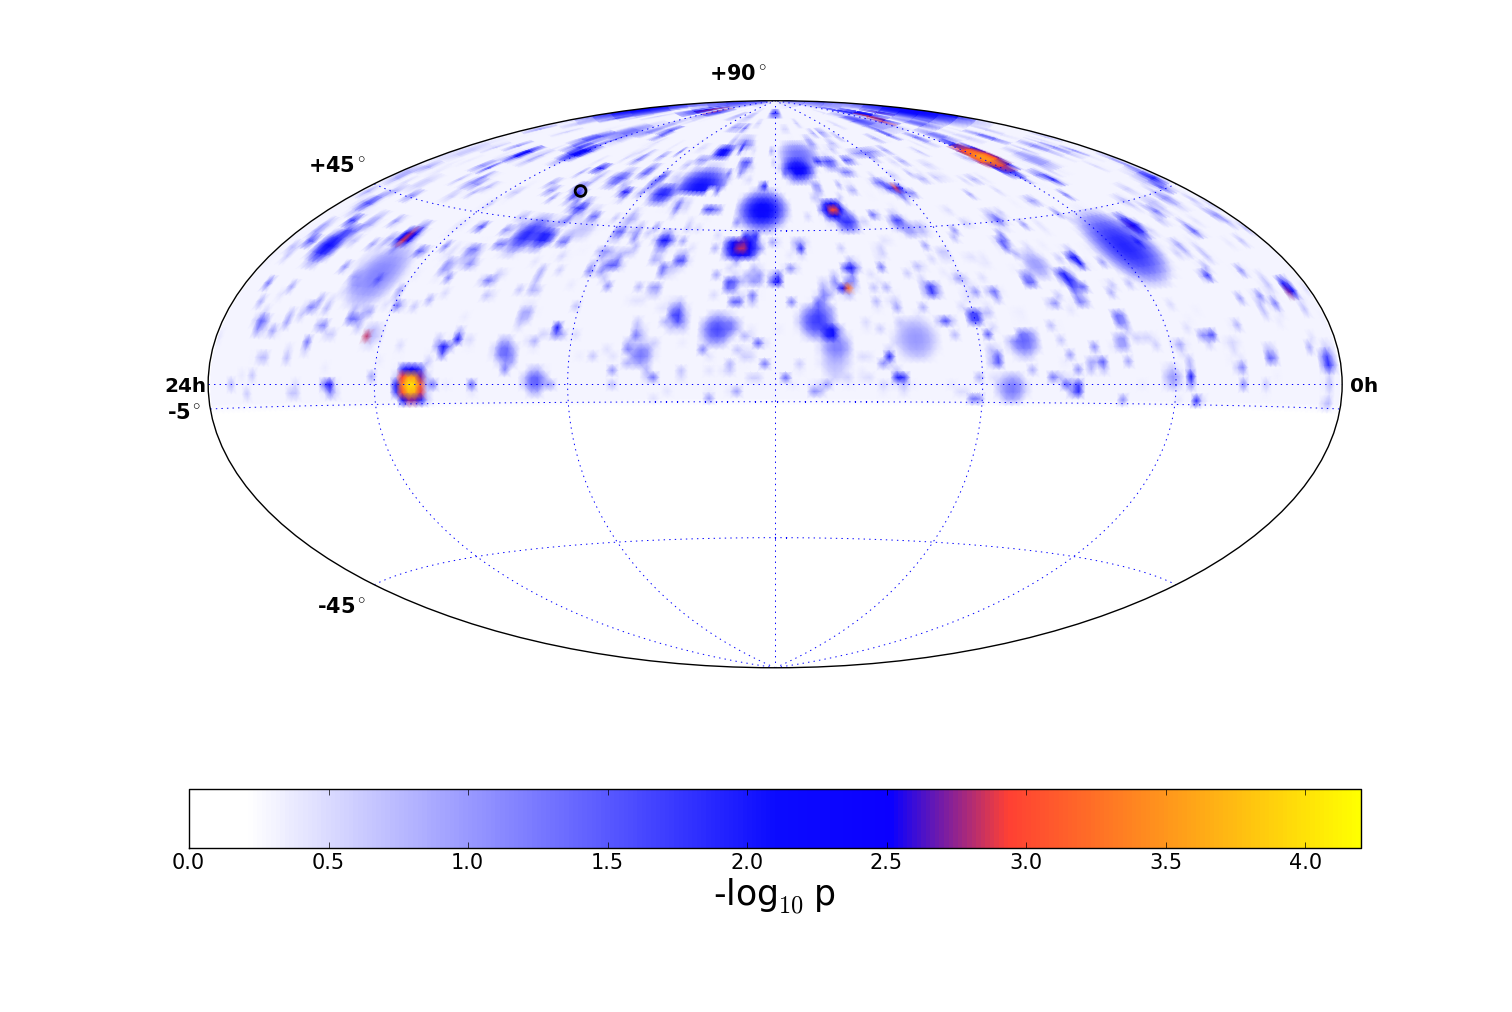
\includegraphics[width=1.0\textwidth,keepaspectratio]{RealResultSkyMap.png}
  \end{center}
  \caption{Sky map of pre-trials p-values for best flares per bin. The black circle identifies the location of the most significant flare found at RA = 268.75$^\circ$ and Declination = 54.25$^\circ$.}
  \label{fig:RealSkyMap}
\end{figure}

\begin{table}[h]
\caption[Best-fit signal parameters]{\label{tab:best_fit_flare}}
\begin{center}
\begin{tabular}{|c|c|}
  \hline
 \textbf{Signal Parameter} &\textbf{ Best-fit Value} \\
\hline
$\hat{n}_s$ & ? \\ \hline
\end{tabular}
\end{center}
\end{table}

%% Post-trials p-value
\begin{figure}[ht]
  \begin{center}
    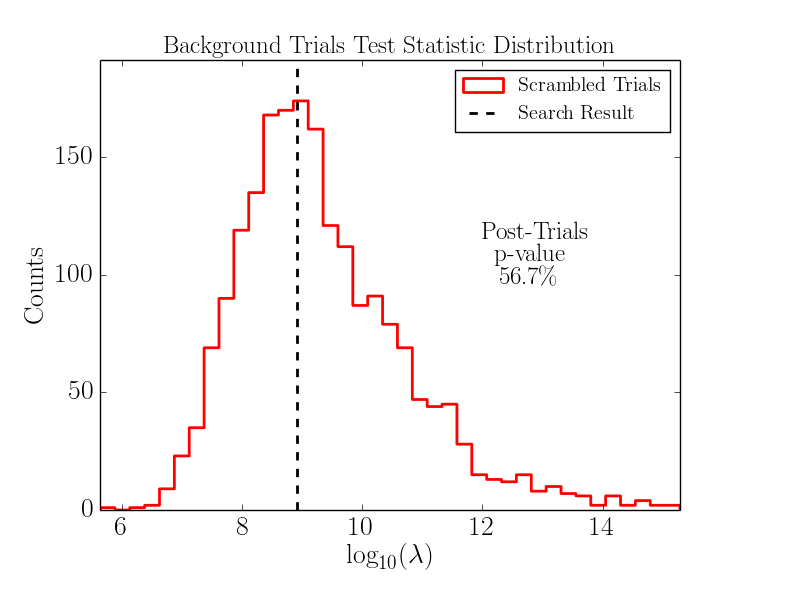
\includegraphics[width=1.0\textwidth,keepaspectratio]{TestStatisticDistribution_WithResult.png}
  \end{center}
  \caption{Distribution of test statistic $\lambda$ of most signficant flare found in 1,985 background trials. The test statistic value for the best fit flare on the unscrambled data set is also plotted.}
  \label{fig:PostTrialsComparison}
\end{figure}

\subsection{Event Upper Limit}

\subsection{Limits on Choked GRBs}

\chapter{Conclusion}

\appendix
\chapter{Appendix A -- Data Selection Process}
Selection of an appropriate event sample required many iterations of trial cuts and background rejection methods. The final established selection criteria were settled on after careful study using Monte Carlo simulation of background and signal events in addition to the real background-dominated data.
\chapter{Appendix B -- Final Level Event Distributions}
This appendix contains distributions of select event parameters for both simulation and real events at the final selection level. The plots here show that the data is mostly well modeled by our neutrino simulation. There are some differences it absolute rate that are largely due to uncertainty in the normalization of the atmospheric neutrino spectrum. 
\begin{figure}\label{fig:FL_nch_by_energy}
\centering
\subfigure[LES Nch-Energy Relation]{\label{fig:i}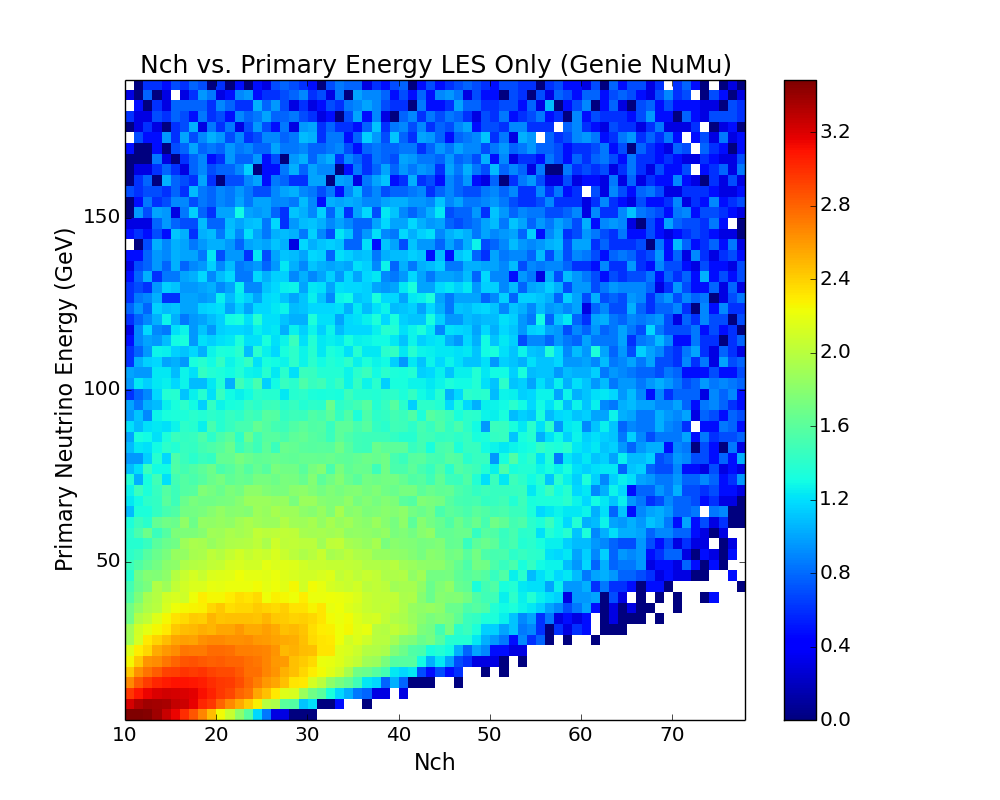
\includegraphics[width=75mm]{FinalLevel_Nch_Vs_Energy_NuMu_LESOnly.png}}
\subfigure[HES Nch-Energy Relation]{\label{fig:ii}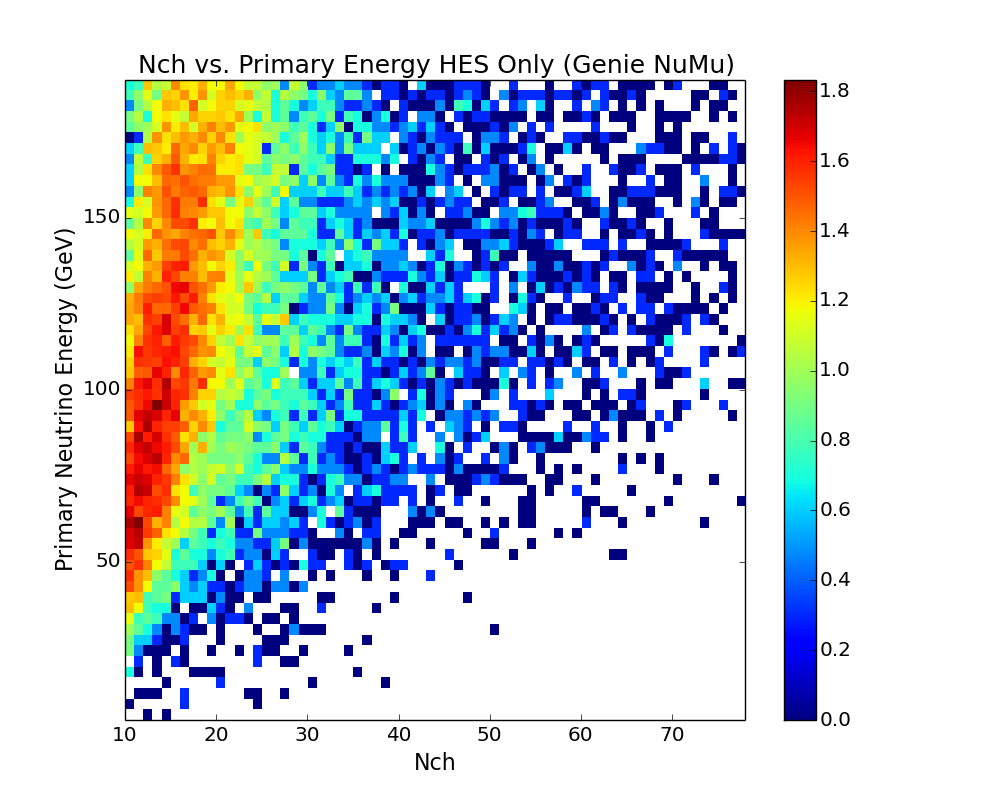
\includegraphics[width=75mm]{FinalLevel_Nch_Vs_Energy_NuMu_HESOnly.png}}
\caption{NCh-Energy relation for simulated $\nu_\mu$ neutrino events at the final level. Nch is a shorthand term for the number of DOMs receiving light from an event. Subfigure (a) shows the correlation for events belonging to the Low-Energy Stream (LES) branch of the event selection while (b) shows the same for events belonging to the High-Energy Stream or HES branch.} 
\end{figure}

\begin{figure}\label{fig:final_level_distros}
\centering
\subfigure[Reconstructed Event Azimuth]{\label{fig:reco_azi}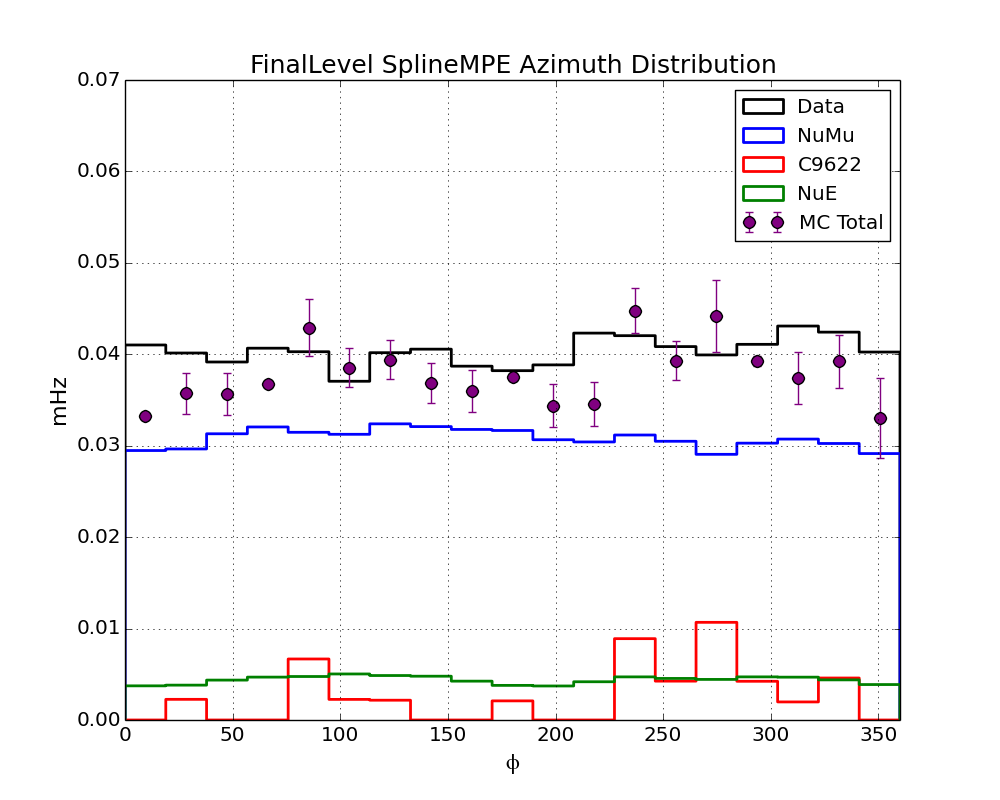
\includegraphics[width=75mm]{LES_SplineMPE_AzimuthDist_FinalLevelDist.png}}
\subfigure[Reconstructed Event Zenith]{\label{fig:reco_zen}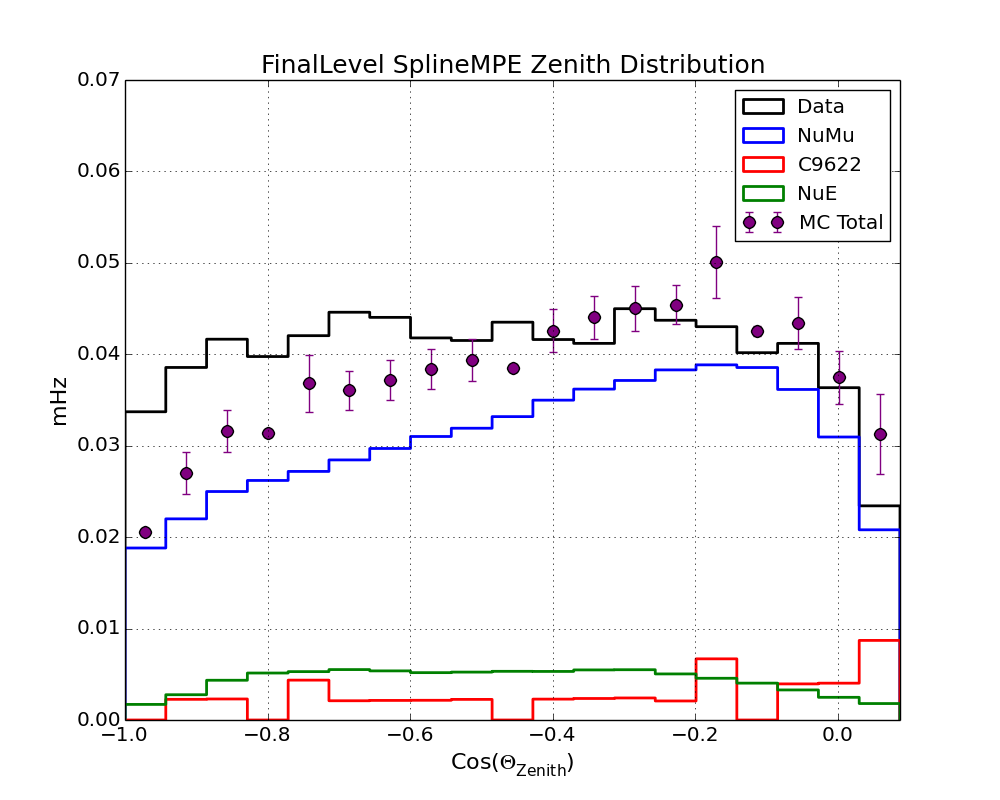
\includegraphics[width=75mm]{LES_SplineMPE_ZenithDist_FinalLevelDist.png}}
\subfigure[Reconstruction Reduced Log-likelihood]{\label{fig:reco_rlogl}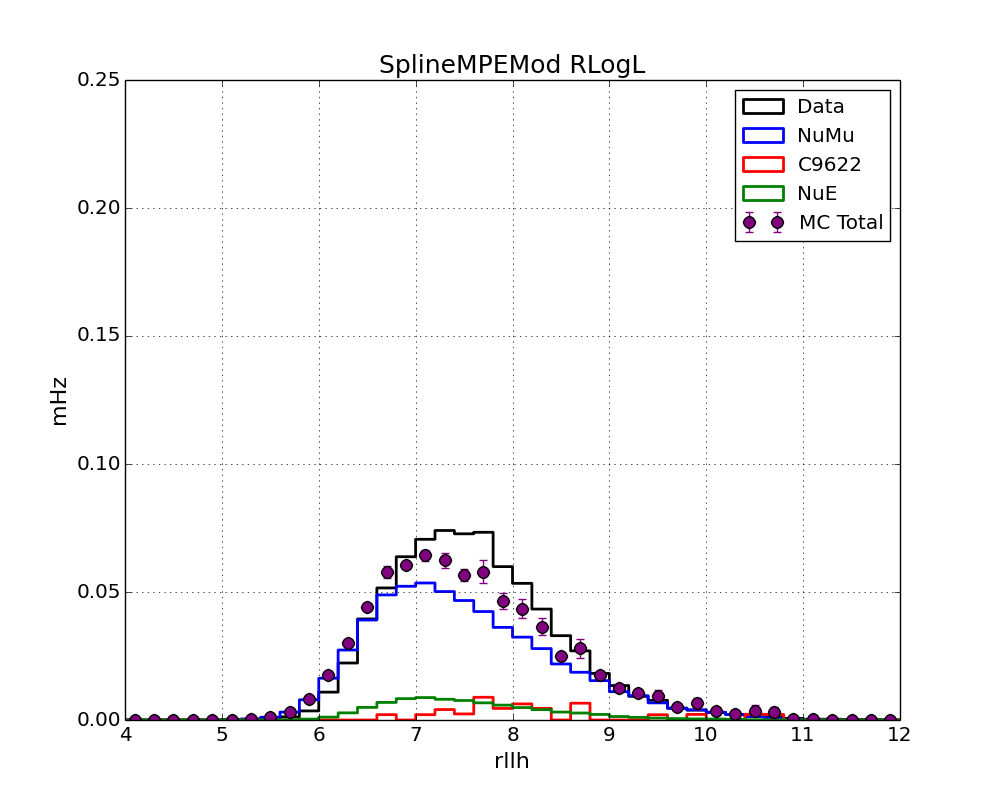
\includegraphics[width=75mm]{LES_BDTParam_SplineMPEMod_RLogL_FinalLevelDist.png}}
\subfigure[Reconstructed Event Vertex Detector Z-position]{\label{fig:reco_z}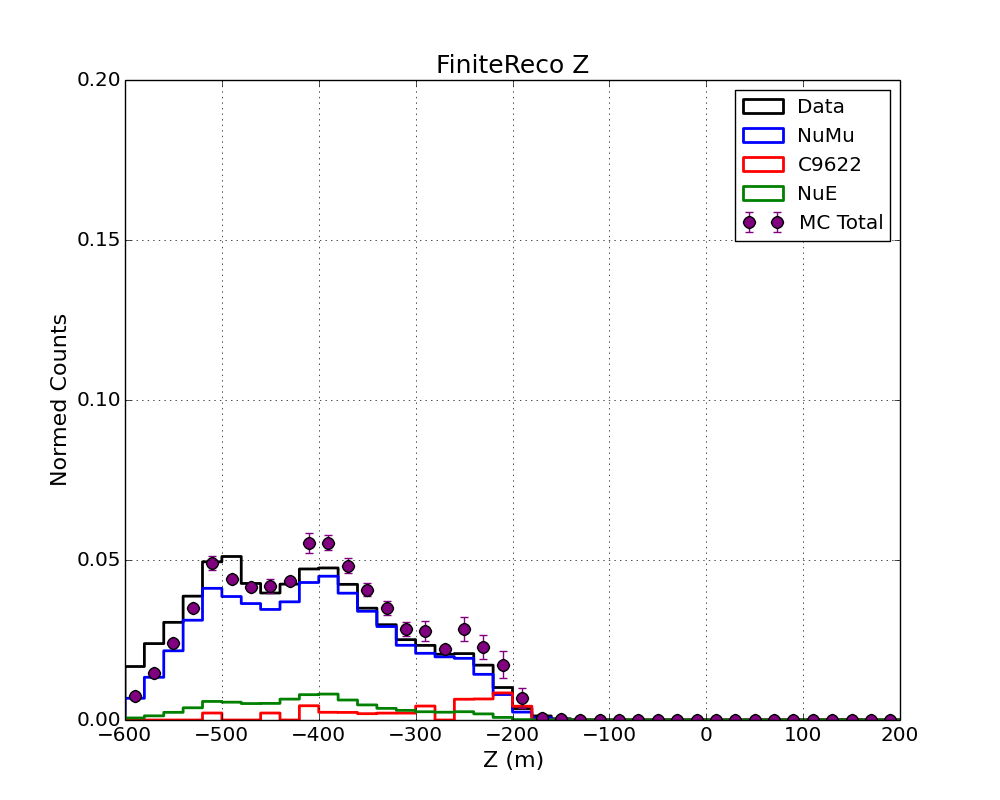
\includegraphics[width=75mm]{LES_BDTParam_FiniteReco_Z_FinalLevelDist.png}}
\caption{Distributions of  for simulation and real data at the final event level. Plots above for the Low-Energy Stream (\textbf{LES}) branch of the event sample.} 
\end{figure}

\begin{postliminary}
\bibliography{jdthesis}{}

\postfacesection{Index}{%
%%             ... generate an index here
%%         look into gatech-thesis-index.sty
}
\begin{vita}

\end{vita}
\end{postliminary}
\end{document}
